\documentclass[10pt]{article}

\usepackage{array}
\usepackage{amsthm}
\usepackage{amsmath}
\usepackage{amssymb}
\usepackage{amsfonts}
\usepackage{stmaryrd}
\usepackage{tikz}
\usepackage{comment}
\usepackage{xspace}
\usepackage{makeidx}
\usepackage{stackengine}
\usepackage{ifthen}
\usepackage{listofitems}
\usepackage{graphicx}
\usepackage[final]{listings}
\usepackage{hyperref}
\usepackage{enumitem}

\graphicspath{ {.} }
\lstset{language=Java,
  commentstyle=\color{brown},
  keywordstyle=\color{blue},
  stringstyle=\color{red},
  basicstyle=\ttfamily}

\lstdefinelanguage{ddlog}{
  language=Java, % we base it on Java, just for comments
  morekeywords={input, output, typedef, relation, typedef, bool, not,
    string, bit, extern, function, var, for, match, skip, in, integer, % not really in DDlog
    Aggregate, FlatMap},
  deletestring=[b]{'}
}
\hypersetup{
  colorlinks   = true,    % Colours links instead of ugly boxes
  urlcolor     = blue,    % Colour for external hyperlinks
  linkcolor    = blue,    % Colour of internal links
  citecolor    = red      % Colour of citations
}
\hypersetup{final}

\usetikzlibrary{shapes, arrows.meta, positioning}
\tikzstyle{block} = [draw, fill=white, rectangle]

\newcommand{\rectangle}[5]{
\ifthenelse{\equal{#1}{1}}{
    \draw[fill=black!20!white] (#2,#3) rectangle(#4, #5);
}{
    \draw (#2,#3) rectangle(#4, #5);
}}

% A single box
\newcommand{\sngl}[1]{
\vcenter{\hbox{
\begin{tikzpicture}[scale=.4]
\rectangle{#1}{0}{0}{1}{1}
\end{tikzpicture}
}}}

% A column vector with two parts:
% a large one and a small one (last element)
% the two arguments are 0 for "empty" and 1 for "filled"
% they correspond to the two parts.  These must be used
% in math mode.
\newcommand{\strm}[1]{
\setsepchar{ }
\readlist\arg{#1}
\vcenter{\hbox{
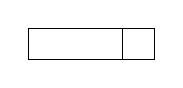
\begin{tikzpicture}[scale=.4]
\rectangle{\arg[1]}{0}{0}{3}{-1}
\rectangle{\arg[2]}{3}{0}{4}{-1}
\end{tikzpicture}
}}}

% A block matrix with 4 zones
\newcommand{\mtrx}[1]{
\setsepchar{ }
\readlist\arg{#1}
\vcenter{\hbox{

\begin{tikzpicture}[scale=.4]
\rectangle{\arg[1]}{0}{0}{3}{-3}
\rectangle{\arg[2]}{3}{0}{4}{-3}
\rectangle{\arg[3]}{0}{-3}{3}{-4}
\rectangle{\arg[4]}{3}{-3}{4}{-4}
\end{tikzpicture}
}}}

\newcommand{\matmult}[2]{\left( #1 \times #2 \right)}

\theoremstyle{definition}
\newtheorem{theorem}{Theorem}[section]
\newtheorem{lemma}[theorem]{Lemma}
\newtheorem{corollary}[theorem]{Corollary}
\newtheorem{definition}[theorem]{Definition}
\newtheorem{proposition}[theorem]{Proposition}
\newtheorem{example}[theorem]{Example}
\newtheorem{algorithm}[theorem]{Algorithm}

\newcommand{\secref}[1]{Section~\ref{#1}}  % reference to a section
\newcommand{\refsec}[1]{\secref{#1}}
% Used when a term is first defined.  Adds the term to the index.
\newcommand{\defined}[1]{\textbf{#1}\index{#1}}
\newcommand{\zr}{$\Z$-set\xspace}
\newcommand{\zrs}{$\Z$-sets\xspace} % plural
\newcommand{\means}[1]{\ensuremath{\llbracket #1 \rrbracket}}
\newcommand{\code}[1]{\mbox{\texttt{#1}}}
\newcommand{\Z}{\mathbb{Z}}  % integers
\newcommand{\R}{\mathbb{R}}  % reals
\newcommand{\N}{\mathbb{N}}  % naturals
\newcommand{\B}{\mathbb{B}}  % Booleans
\newcommand{\norm}[1]{\| #1 \|} % norm; requires math mode
% stream with elements of a given type
\newcommand{\stream}[1]{\ensuremath{\mathcal{S}_{#1}}}
% finite stream with elements of a given type (zero almost everywhere)
\newcommand{\streamf}[1]{\ensuremath{\overline{\mathcal{S}_{#1}}}}
\newcommand{\zm}{\ensuremath{z^{-1}}} % stream delay operator
\ifthenelse{\equal{1}{0}}{ % allows switching to mathit/mathcal
\newcommand{\I}{\mathcal{I}}  % stream integration
\newcommand{\D}{\mathcal{D}}  % stream derivative
}{
\newcommand{\I}{\mathit{I}}  % stream integration
\newcommand{\D}{\mathit{D}}  % stream derivative
}
\newcommand{\inc}[1]{{#1}^{\Delta}}
\newcommand{\dbsp}{DBSP\xspace}
\newcommand{\distinct}{\mathit{distinct}}  % distinct operator
% set with elements of given type
\newcommand{\set}[1]{\mathit{set}_{#1}}
\newcommand{\id}{\ensuremath{\mathit{id}}} % identity function
\newcommand{\isset}{\mbox{isset}}
\newcommand{\ispositive}{\mbox{ispositive}}
\newcommand{\defn}{\stackrel{\textrm{\scriptsize def}}{=}}
\newcommand{\map}{\mbox{map}}
\newcommand{\fix}[2]{\mbox{fix}\,#1.#2}
\newcommand{\lift}[1]{{\uparrow}#1}
\newcommand{\rew}{\ensuremath{\mapsto}} % rewriting
\newcommand{\birew}{\ensuremath{\mapsfrom\!\mapsto}} % bidirectional rewriting
\newcommand{\pair}[2]{\ensuremath{\langle #1,#2 \rangle}} % pairing
\newcommand{\zpp}[1]{\mbox{zpp}(#1)}
\newcommand{\makeset}{\ensuremath{\mbox{makeset}}}
\newcommand{\sv}[1]{ % simple stream value, supplied as a space-separated list of 5 values
\setsepchar{ }
\readlist\arg{#1}
{[}
\begin{array}{cccccc}
    \arg[1] & \arg[2] & \arg[3] & \arg[4] & \arg[5] & \cdots
\end{array}
{]}
}

\newcommand{\st}{\;|\;}
\newcommand\Hookarrowleft[1]{\ensuremath{\stackrel{\curvearrowleft}{#1}}}

\newcommand{\cut}[2]{#1|_{_{\leq #2}}}
\newcommand{\scut}[2]{#1|_{_{< #2}}}


\setlength{\marginparwidth}{4cm}
\newcommand{\scream}[2]{\marginpar{\footnotesize \textbf{#1}: #2}}
\newcommand{\val}[1]{\scream{VAL}{#1}}
\newcommand{\mihai}[1]{\scream{MIHAI}{#1}}
\newcommand{\leonid}[1]{\scream{LEONID}{#1}}

\title{\dbsp: Automatic Incremental View Maintenance for Rich Query
Languages}
\author{
  Mihai Budiu \\ VMware Research \and
  Tej Chajed \\ VMware Research \and
Frank McSherry \\ Materialize Inc. \and
Leonid Ryzhyk \\ VMware Research \and
Val Tannen \\ University of Pennsylvania
}

\makeindex
\begin{document}

\maketitle

\begin{abstract}
Incremental view maintenance (IVM) has been for a long time a central problem in database theory~\cite{gupta-idb95}.
Many solutions have been proposed for restricted classes of database languages,
such as the relational algebra, or Datalog.  These techniques do not naturally generalize to
richer languages.  In this paper we give a general, heuristic-free
solution to this problem in 3 steps: (1) we describe a simple but expressive language
called \dbsp for describing computations over data streams; (2) we give a new mathematical definition of IVM and
a general algorithm for solving IVM for arbitrary \dbsp programs, and (3) we show
how to model many rich database query languages (including the full relational algebra, queries over
sets and multisets, arbitrarily nested relations, aggregation, flatmap (unnest), monotonic and non-monotonic
recursion, streaming aggregation, and arbitrary compositions of all of these) using \dbsp.
As a consequence, we obtain efficient
incremental view maintenance algorithms for queries over all these languages.
\end{abstract}

\begin{quote}
This document is work in progress.  It contains a formal specification
of the \dbsp language, proofs of the theoretical results, and the
specification of several query languages in \dbsp.  A shorter earlier
preprint is available at \url{https://arxiv.org/abs/2203.16684}.
\end{quote}

\tableofcontents

\section{Introduction}\label{sec:introduction}

\subsection{Incremental computation}\label{sec:intro-incremental}

Incremental view maintenance (IVM) is an important and well-studied
problem in databases~\cite{gupta-idb95}.  The IVM problem can be
stated as follows: we are given a large database $DB$ (say 1 billion
records) and a view $V$, described by a query $Q$.  The goal of IVM is
to keep the contents of $V$ up-to-date in response to changes of the
database.

As a concrete example, consider the following view definition
statement in SQL: \texttt{CREATE VIEW V AS SELECT * FROM T WHERE Age
  >= 10}.  In this example the query $Q$ defining the view $V$ is
\texttt{SELECT * FROM T WHERE Age >= 10}.  The view \code{V} always
contains all the rows of table \code{T} whose value for the column
\code{Age} is greater than or equal to 10.

In general a query is a function applied to the database state: $V =
Q(DB)$.  A na\"ive solution re-executes query $Q$ every time the
database changes, illustrated in the following diagram.  Time is the
horizontal axis; the horizontal arrows labeled with $\Delta$ depict
changes to the database, which we assume are much smaller than the
database itself (e.g., a change could touch perhaps 100 records).  The
``up'' arrows show the re-evaluation of $Q$ for each database
snapshot.


\includegraphics[trim={0 4.8in 3.7in 0},clip,scale=.30]{view.pdf}

The naive solution is expensive.  After the first version of the view
has been constructed, an ideal algorithm would compute only
\emph{changes} to the view $\Delta V$ doing work $O(|\Delta DB|)$.
Ideally, we want to construct a new query $\inc{Q}$ with the property
that $\Delta V = \inc{Q}(\Delta DB)$, i.e., $\inc{Q}$ can compute the
change of the view from the change of the database:

\includegraphics[trim={0 5.2in 4.1in 0},clip,scale=.30]{incview.pdf}

We call $\inc{Q}$ the \emph{incremental} version of $Q$.  If one
thinks of $\inc{Q}$ as a function of $\Delta DB$, one can show that
the ideal solution as described above is impossible to reach.

In this paper we propose a new way to define $\inc{Q}$, as a form of
\emph{computation on streams}.  Our model is inspired by Digital
Signal Processing DSP~\cite{rabiner-book75}, applied to databases,
hence the name \dbsp.  $\inc{Q}$ can be very efficient.  As for
traditional database queries, the performance of $\inc{Q}$ depends
both on the query $Q$ but also on the actual data that the query is
applied to.  Informally, $\inc{Q}$ built by our algorithm, is faster
than $Q$ by a factor of $O(|DB| / |\Delta DB|)$.  In practice this may
be an improvement of several orders of magnitude.  For our example
above $|DB| \approx 10^9$ and $|\Delta DB| \approx 10^2$, this can
make $\inc{Q}$ \textbf{10 million times} faster!

Instead of treating the database as a large changing object, we model
it as a \emph{sequence} or \emph{stream} of database snapshots.
Similarly, consecutive view snapshots form a stream.  \dbsp is a
simple programming language computing on \\streams; inputs and outputs
are streams of arbitrary values.

%Whereas previous IVM solutions are based on defining a notion of a
%(partial) derivative of $Q$ with respect to its inputs, our definition
%only requires computing \emph{derivatives of streams} as functions of
%time.  Derivatives of streams are always well-defined if the data
%computed on has a notion of difference that satisfies some simple
%mathematical properties --- specifically, that it forms a commutative
%group.  (Fortunately, relational databases can be modeled in such a
%way~\cite{green-pods07, koch-pods10}.)

The \dbsp language has only 4 operators.  However, it can express a
rich set of computations on streams, including repeated computations
(similar to the repeated queries $Q$ above), recursive computations
that compute fixed points (like Datalog programs), streaming
computations, and incremental computations (which we define shortly).
The full paper~\cite{budiu-vldb23} gives a precise mathematical
description of \dbsp, this presentation is simplified to convey the
main intuitions.  We omit the related work section from this
presentation.

The central result of this paper is Algorithm~\ref{algorithm-inc}
which, given a \dbsp program that computes on a stream of values,
mechanically transforms it into an incremental \dbsp program that
computes on a stream of changes.

\dbsp is not tied to databases in any way; it is in fact a
Turing-complete language that can be used for many other purposes.
But it works particularly well in the area of databases, for two
reasons:

\begin{itemize}[nosep, leftmargin=0pt, itemindent=0.5cm]
  \item \dbsp operates on values from a commutative group.  Databases
    can be modeled as a commutative group.
  \item \dbsp reduces the problem of incrementalizing a complex
    program to the problem of incrementalizing each primitive
    operation that appears in the program.  For databases there are
    known efficient incremental implementations for all primitive
    operations.
\end{itemize}

%\dbsp has several attractive properties:
%
%\begin{enumerate}
%\item it is \textbf{simple}.  \dbsp has only 4 operators, and it is
%  built entirely on elementary concepts such as functions and
%  algebraic groups.
%\item it is \textbf{expressive}.  It can be used to define precisely
%  multiple concepts: traditional queries, streaming computations, and
%  incremental computations.
%\item mathematically \textbf{precise}.  All the results in this paper
%  have been formalized and checked using the Lean proof
%  assistant~\cite{moura-cade15}.
%\item it is \textbf{modular}, in the following two ways:
%(a) the incremental version of a complex query can be reduced
%recursively to incrementalizing its component subqueries.
%This gives a simple, syntactic,
%heuristic-free algorithm (Algorithm~\ref{algorithm-inc})
%that converts an arbitrary \dbsp query plan to its incremental form.
%(b) Extending \dbsp to support new primitive operators is easy,
%and they immediately benefit from the rest of the theory of
%incrementalization.
%An important consequence of modularity is that the theory
%can be efficiently implemented, as we
%briefly discuss in \refsec{sec:implementation}.
%\end{enumerate}

\subsection{Circuits and Streams}\label{sec:intro-circuits}

In this paper we use circuit diagrams to depict programs.  In a
circuit a rectangle represents a function, and an arrow represents an
input or output value.  The following diagram shows a function $f$
consuming two inputs $i$ (input 0) and $j$ (input 1) and producing one
output $o = f(i, j)$:
%
\begin{center}
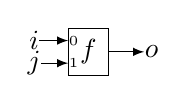
\begin{tikzpicture}[auto,>=latex,inner sep=0mm]
  \node[block, minimum height=.6cm, minimum width=.5cm] (function) {$f$};
  \node[below=1mm of function.north west,font=\tiny,anchor=north west] (0) {0};
  \node[above=1mm of function.south west,font=\tiny,anchor=south west] (1) {1};
  \node[left of=0, node distance=.5cm] (input0) {$i$};
  \node[left of=1, node distance=.5cm] (input1) {$j$};
  \node[right of=function, node distance=.8cm] (output) {$o$};
  \draw[->] (input0) -- (0);
  \draw[->] (input1) -- (1);
  \draw[->] (function) -- (output);
\end{tikzpicture}
\end{center}
\vspace{-1.2ex}
%
Most of the functions we deal with are commutative, so we can skip
inputs label, displaying the circuit above as:
%
\begin{center}
  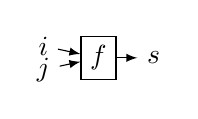
\begin{tikzpicture}[auto,>=latex, node distance=.7cm]
    \node[] (input0) {$i$};
    \node[below of=input0,node distance=.15cm] (dummy) {};
    \node[below of=dummy,node distance=.15cm] (input1) {$j$};
    \node[block, right of=dummy] (T) {$f$};
    \node[right of=T] (output) {$s$};
    \draw[->] (input0) -- (T);
    \draw[->] (input1) -- (T);
    \draw[->] (T) -- (output);
  \end{tikzpicture}
\end{center}
\vspace{-1.2ex}
%
Functions, and their circuits, can be composed, as in the following
example for the function $o = g(s) + (f(s) \times s)$:
%
\begin{center}
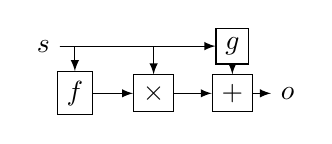
\begin{tikzpicture}[auto,>=latex]
  \node[] (input) {$s$};
  \node[] [right of=input, node distance=.4cm] (dummy) {};
  \node[block, below of=dummy, node distance=.6cm] (S1) {$f$};
  \node[block, right of=S1] (T1) {$\times$};
  \node[block, right of=T1] (T2) {$+$};
  \node[block, above of=T2, node distance=.6cm] (S2) {$g$};
  \node[right of=T2, node distance=.7cm] (output) {$o$};
  \draw[->] (input) -| (S1);
  \draw[->] (input) -| (T1);
  \draw[->] (S1) -- (T1);
  \draw[->] (T1) -- (T2);
  \draw[->] (input) -- (S2);
  \draw[->] (T2) -- (output);
  \draw[->] (S2) -- (T2);
\end{tikzpicture}
\end{center}
\vspace{-1ex}
%
We say that two circuits are \defined{equivalent} if they compute the
same function.  We use the symbol $\cong$ to indicate circuit
equivalence.  For example, we have the following circuit equivalence
(where $\circ$ is function composition):

\noindent
\begin{tabular}{m{3cm}m{.3cm}m{3cm}c}
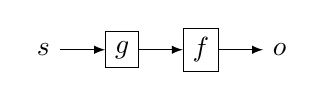
\begin{tikzpicture}[auto,>=latex]
  \node[] (input) {$s$};
  \node[block, right of=input] (g) {$g$};
  \node[block, right of=g] (f) {$f$};
  \node[right of=f] (output) {$o$};
  \draw[->] (input) -- (g);
  \draw[->] (g) -- (f);
  \draw[->] (f) -- (output);
\end{tikzpicture}
&
$\cong$
&
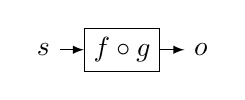
\begin{tikzpicture}[auto,>=latex]
    \node[] (input) {$s$};
    \node[block, right of=input, node distance=1cm] (fg) {$f \circ g$};
    \node[right of=fg, node distance=1cm] (output) {$o$};
    \draw[->] (input) -- (fg);
    \draw[->] (fg) -- (output);
\end{tikzpicture}
&
(*)
\end{tabular}
\vspace{-2ex}

\subsection{Streams}

The core notion of \dbsp is the \textbf{stream}.  Given a set $A$, a
\defined{stream} \emph{of values from $A$} is an infinite sequence of
values from $A$.  $\stream{A}$ denotes the set of all streams with
values from $A$.  We write $s[t]$ for the $t$-th element of the stream
$s$.  Think of $t$ as the ``time'' and of $s[t]\in A$ as the value of
the stream $s$ ``at time'' $t$.  We show streams as a sequence of
boxes, with time from \emph{right to left}: e.g., the stream $s[t] =
t$ is:
%
\begin{center}
\begin{tabular}{cc}
  \sv{0 1 2 3 4} \\
  $\xleftarrow[\hspace{1cm}\mathrm{time}\hspace{1cm}]{}$
\end{tabular}
\end{center}
\vspace{-1ex}
%
%\begin{definition}[stream operator]
A \defined{stream operator} is a function that computes on streams and
produces streams.
%\end{definition}
In general we use ``operator'' for streams, and ``function'' for
computations on ``scalar'' values.

We use arrows with a double head to depict streams.  The following
diagram shows a stream operator $T$ consuming two input streams $s_0$
and $s_1$, producing one output stream $s$:
%
\begin{center}
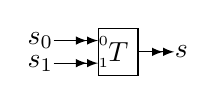
\begin{tikzpicture}[auto,>=latex,inner sep=0mm]
  \node[block, minimum height=.6cm, minimum width=.5cm] (function) {$T$};
  \node[below=1mm of function.north west,font=\tiny,anchor=north west] (0) {0};
  \node[above=1mm of function.south west,font=\tiny,anchor=south west] (1) {1};
  \node[left of=0, node distance=0.8cm] (input0) {$s_0$};
  \node[left of=1, node distance=0.8cm] (input1) {$s_1$};
  \node[right of=function, node distance=.8cm] (output) {$s$};
  \draw[->>] (input0) -- (0);
  \draw[->>] (input1) -- (1);
  \draw[->>] (function) -- (output);
\end{tikzpicture}
\vspace{-1ex}
\end{center}
%
We write $s = T(s_0, s_1)$.
%\begin{definition}(lifting)
Given a function $f: A \to B$, we define a stream operator $\lift{f}
:\stream{A} \to \stream{B}$ (read as ``$f$ lifted'') by applying
function $f$ to each input value independently:
\begin{center}
  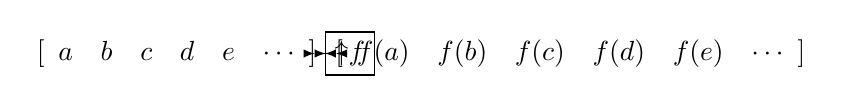
\begin{tikzpicture}[auto,>=latex]
    \node[] (input) {$\sv{a b c d e}$};
    \node[block, right of=input, node distance=2.2cm] (f) {$\lift{f}$};
    \node[right of=f, node distance=2.8cm] (output) {$\sv{f(a) f(b) f(c) f(d) f(e)}$};
    \draw[->>] (input) -- (f);
    \draw[->>] (f) -- (output);
  \end{tikzpicture}
\end{center}
\vspace{-1ex}
%\end{definition}

To simplify the notation, we write $a + b$ for streams $a, b$ instead
of $a (\lift{+}) b$; we also write $-a$ instead of $(\lift{-})a$.

\subsection{Databases as streams}

We generally think of streams as sequences of ``small'' values, such
as insertions or deletions in a database.  However, we also treat the
whole database as a \emph{stream of database snapshots}.  We model a
database as a stream $DB$.  Time is not wall-clock time, but counts
the transactions applied to the database.  Since transactions are
linearizable, they have a total order.  $DB[t]$ is the snapshot of the
database contents after $t$ transactions have been applied.  This
notation is apparent in the diagrams in \refsec{sec:intro-incremental}.

Database transactions also form a stream $\Delta DB$, this time a
stream of \emph{changes}, or \emph{deltas}, that are applied to the
database.  The values of this stream are defined by $(\Delta DB)[t] =
DB[t] - DB[t-1]$, where ``$-$'' stands for the difference between two
databases, a notion that we will soon make more precise.  The $\Delta
DB$ stream can be produced from the $DB$ stream by the \emph{stream
differentiation} operator $\D$; this operator produces as its output
the stream of changes from its input stream; we have thus $\D(DB) =
\Delta DB$.

Conversely, the database snapshot at time $t$ is the cumulative result
of applying all transactions up to $t$: $DB[t] = \Delta DB[0] + \Delta
DB[1] + \ldots + \Delta DB[t]$.  The stream operator $\I$ is defined
to produce each output by adding up all previous inputs.  We call $\I$
\emph{stream integration}, the inverse of differentiation.  The
following diagram shows the relationship between the streams $\Delta
DB$ and $DB$:
\begin{center}
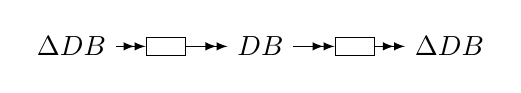
\begin{tikzpicture}[auto,>=latex,minimum width=.5cm, node distance=1.2cm]
  \node[] (input) {$\Delta DB$};
  \node[block, right of=input] (I) {$\I$};
  \node[right of=I] (output) {$DB$};
  \node[block, right of=output] (D) {$\D$};
  \node[right of=D] (end) {$\Delta DB$};
  \draw[->>] (input) -- (I);
  \draw[->>] (I) -- (output);
  \draw[->>] (output) -- (D);
  \draw[->>] (D) -- (end);
\end{tikzpicture}
\end{center}

A view in this model is also a stream.  Suppose query $Q$ defining a
view $V$.  For each snapshot of the database stream we have a snapshot
of the view: $V[t] = Q(DB[t])$.  A view is thus just a lifted query:
$V = (\lift{Q})(DB)$.

Armed with these basic definitions, we can precisely define IVM.  What
does it mean to maintain a view incrementally?  A maintenance
algorithm needs to compute the \emph{changes} to the view given the
changes to the database. Given a query $Q$, a key contribution of this
paper is the definition of its \emph{incremental version} $\inc{Q}$,
using stream integration and differentiation, depicted graphically as:
\vspace{-2ex}
%
\begin{center}
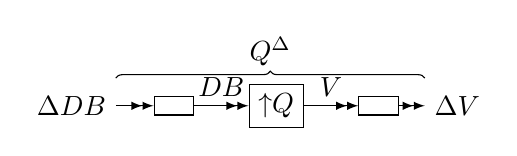
\begin{tikzpicture}[auto,>=latex,minimum width=.5cm]
  \node[] (input) {$\Delta DB$};
  \node[block, right of=input, node distance=1.3cm] (I) {$\I$};
  \node[block, right of=I, node distance=1.3cm] (Q) {$\lift{Q}$};
  \node[block, right of=Q, node distance=1.3cm] (D) {$\D$};
  \node[right of=D] (output) {$\Delta V$};
  \draw[->>] (input) -- (I);
  \draw[->>] (I) -- node (db) {$DB$} (Q);
  \draw[->>] (Q) -- node (B) {$V$} (D);
  \draw[->>] (D) -- (output);
  \draw[decorate, decoration = {brace, raise=10pt}] (input) -- (output)
  node[pos=.5, above=11pt]{$\inc{Q}$};
\end{tikzpicture}
\end{center}
\vspace{-1ex}
%
Mathematically: $\inc{Q} = \D \circ (\lift{Q}) \circ \I$.  The
incremental version of a query $Q$ is a \emph{streaming operator}
$\inc{Q}$ which computes directly on changes and produces changes.
The incremental version of a query is thus always well-defined.  The
above definition gives us one way to compute a query incrementally,
but applying it naively produces an inefficient execution, since it
reconstructs the database at each step.  It is in fact as bad as the
naive solution.  In \refsec{sec:incremental} we show how we can
optimize the implementation of $\inc{Q}$. The key property is that the
we can ``push'' the $\inc{.}$ operator ``down'' in a query plan:
$\inc{(Q_1 \circ Q_2)} = \inc{Q_1} \circ \inc{Q_2}$.

Armed with this general theory of incremental computation, in
\secref{sec:relational} we show how to model relational queries in
\dbsp.  This immediately gives us a general algorithm to compute the
incremental version of any relational query.  These results were
previously known, but they are cleanly modeled by \dbsp.
\secref{sec:recursion} shows how programs containing recursion can be
implemented and incrementalized in \dbsp.  For example, given an
implementation of transitive closure in the natural recursive way, our
algorithm produces a program that efficiently maintains the transitive
closure of a graph as nodes and edges are added and deleted.

\subsection{Contributions}

This work makes the following contributions:
\begin{enumerate}[nosep, leftmargin=0pt, itemindent=0.5cm, label=\textbf{(\arabic{*})}]
  \item We introduce \dbsp, a simple but expressive language for
    streaming computation. \dbsp gives an elegant formal foundation
    unifying the manipulation of streaming and incremental
    computations.
  \item An algorithm for incrementalizing any streaming computation
    expressed in \dbsp that handles arbitrary insertions and deletions
    from any of the data sources.
  \item An illustration of how \dbsp can model various classes of
    practical queries, such as relational algebra, nested relations,
    aggregations, and Datalog.
  \item The first general and machine-checked theory of IVM.  All the
    theoretical results in the original version of this
    paper~\cite{budiu-vldb23} have been checked~\cite{dbsp-theory}
    using the Lean proof assistant~\cite{moura-cade15}.
  \item A practical open-source implementation of this theory as a
    runtime and a SQL compiler.
\end{enumerate}


\section{Related work}\label{sec:related}

Incremental view maintenance~\cite{gupta-sigmod93, griffin-sigmod95, chaudhuri-icde95,
gupta-idb95, chirkova-book12} is a much studied problem in databases.
A survey of results for Datalog queries is present in~\cite{motik-ai19}.
The standard approach is as follows: given a query $Q$, discover a ``delta query'',
a ``differential'' version $\Delta Q$ that satisfies the equation:
$Q(d+\Delta d)=Q(d)+\Delta Q(d,\Delta d)$, and which can be used to compute
the change for a new input reusing the previous output.
DBToaster introduced recursive recursive IVM~\cite{ahmad-vldb09, koch-pods10}, where
the incrementalization process is repeated for the delta query.

Many custom algorithms were published for various classes of queries: e.g.~\cite{koch-pods16}
handles positive nested relational calculus.  DYN~\cite{idris-sigmod17}
and IDYN~\cite{idris-vldb18, idris-sigmod19} focus on acyclic conjunctive queries.  Instead
of keeping the output view materialized they build data structures that allow efficiently
querying the output views.  PAI maps~\cite{abeysinghe-sigmod22} are specially
designed for queries with correlated aggregations.
AJU~\cite{wang-sigmod20} focuses on foreign-key joins.  It is a matter
of future work to evaluate whether custom \dbsp operators
can match the efficiency of systems specialized for narrow classes
of queries.

\dbsp is a bottom-up system, which always produces eagerly
the \emph{changes} to the output views.
Instead of maintaining the output view entirely, \dbsp proposes
generating deltas as the output of the computation (similar to the kSQL~\cite{jafarpour-edbt19}
\texttt{EMIT CHANGES} queries).  The idea that both
inputs and outputs to an IVM system are streams of changes
seems trivial, but this is key to the symmetry of our solution:
both in our definition of IVM~(\ref{def:inc}), and the fundamental
reason that the chain rule exists --- the chain rule is the one that makes our
structural induction IVM algorithm possible.

Several IVM algorithms for Datalog-like languages use counting based
approaches~\cite{Dewan-iis92,motik-aaai15} that maintain the number of derivations of each
output fact: DRed~\cite{gupta-sigmod93} and its variants~\cite{Ceri-VLDB91,Wolfson-sigmod91,
Staudt-vldb96,Kotowski-rr11,Lu-sigmod95,Apt-sigmod87}, the backward-forward algorithm
and variants~\cite{motik-aaai15,Harrison-wdd92,motik-ai19}.
\dbsp is more general,
and our incrementalization algorithm handles arbitrary recursive queries and
generates more efficient plans for recursive queries
in the presence of arbitrary updates (especially deletions, where competing approaches
may over-delete).  Interestingly, the \zrs weights in \dbsp are related
to the counting-number-of-derivations approaches, but our use of the $\distinct$
operator shows that precise counting is not necessary.

Picallo et al.~\cite{picallo-scop19} provide a general solution to IVM for
rich languages.  \dbsp requires a group structure on the values operated on;
this assumption has two major practical benefits: it simplifies the mathematics considerably
(e.g., Picallo uses monoid actions to model changes), and it provides a general, simple
algorithm (\ref{algorithm-inc}) for incrementalizing arbitrary programs.  The downside of
\dbsp is that one has to find a suitable group structure (e.g., \zrs for sets) to ``embed''
the computation.  Picallo's notion of ``derivative'' is not unique: they need creativity to choose
the right derivative definition, we need creativity to find the right group structure.

Finding a suitable group structure has proven easy for relations (both~\cite{koch-pods10}
and~\cite{green-tcs11} use \zrs to uniformly model data and insertions/deletions), but it is
not obvious how to do it for other data types, such as sorted collections, or tree-shaped
collections (e.g., XML or JSON documents)~\cite{foster-planx08}.  An intriguing question
is ``what other interesting group structures could this be applied to besides \zrs?''
Papers such as~\cite{nikolic-icmd18} explore other possibilities, such as matrix algebra,
linear ML models, or conjunctive queries.

\dbsp does not do anything special for triangle queries~\cite{kara-tds20}.  Are there
better algorithms for this case?

In \secref{sec:extensions} we have briefly mentioned that \dbsp can easily
model window and stream database queries~\cite{arasu-tr02,aurora}; it is an
interesting question whether there are CQL queries that cannot be expressed in \dbsp
(we conjecture that there aren't any).

\citet{bonifati-iclp2018} implemented a verified IVM algorithm for a particular
class of graph queries called Regular Datalog, with an implementation machine-checked in the
Coq proof assistant. Their focus is on a particular algorithm and the approach does not
consider other SQL operators, general recursion, or custom operators (although it is modular
in the sense that it works on any query by incrementalizing it recursively). Furthermore,
for all queries a deletion in the input change stream requires running the non-incremental
query to recover.  We formally verify the theorems in our paper, which
are much broader in scope, but not our implementations.

\dbsp is also related to Differential Dataflow (DD)~\cite{mcsherry-cidr13, murray-sosp13}
and its theoretical foundations~\cite{abadi-fossacs15} (and recently~\cite{mcsherry-vldb20,chothia-vldb16}).
DD's computational model is more powerful than
\dbsp, since it allows time values to be part of an arbitrary lattice.
In fact, DD is the only other framework which we are aware of that can incrementalize
recursive queries as efficiently as \dbsp does.
In contrast, our model uses either ``linear'' times, or nested time dimensions via the modular lifting transformer ($\lift{}$).
\dbsp can express both
incremental and non-incremental computations.  Most importantly, \dbsp comes with Algorithm~\ref{algorithm-inc}, a syntax-directed translation that can convert
any expressible query into an incremental version --- in DD users have
to assemble incremental queries manually using incremental operators.
(materialize.com offers a product that automates incrementalization
for SQL queries based on DD.  Differential Datalog~\cite{ryzhyk-datalog19}
does it for a Datalog dialect.)  Unlike DD, \dbsp is a modular theory,
which easily accommodates the addition of new operators:  as long as we can
express a new operator as a \dbsp circuit, we can (1) define its incremental version,
(2) apply the incrementalization algorithm to obtain an efficient
incremental implementation, and (3) be confident that it composes with any
other operators.


\part{Streaming and incremental computations}
\section{Stream operators}\label{sec:streams}

%\subsection{Useful stream operators}\label{sec:abelian}

For the rest of this paper we require the set of values $A$ of a
stream $\stream{A}$ to form a commutative group, with operations $+$,
$-$, and a $0$ (zero) value.  The \emph{plus} defines what it means to
\emph{add} new data, while the \emph{minus} allows us to compute
differences (deltas).  We show later that this requirement is not a
problem for using \dbsp in the context of databases.

Stream operators are very powerful mathematically, but in \dbsp we
restrict ourselves to a very small subset.  All \dbsp computations are
\emph{causal}~\cite{causal}: the output at time $t$ is produced
immediately after all inputs up at time $t$ have been received; the
output at time $t$ cannot depend on inputs arriving after $t$.

The following circuit equivalence tells us that we can lift a circuit
by lifting each of its functions separately:

\noindent
\begin{tabular}{m{3cm}m{.3cm}m{3cm}c}
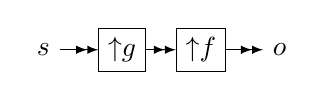
\begin{tikzpicture}[auto,>=latex]
  \node[] (input) {$s$};
  \node[block, right of=input] (g) {$\lift{g}$};
  \node[block, right of=g] (f) {$\lift{f}$};
  \node[right of=f] (output) {$o$};
  \draw[->>] (input) -- (g);
  \draw[->>] (g) -- (f);
  \draw[->>] (f) -- (output);
\end{tikzpicture}
&
$\cong$
&
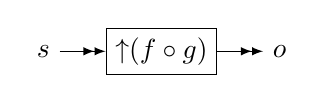
\begin{tikzpicture}[auto,>=latex]
    \node[] (input) {$s$};
    \node[block, right of=input, node distance=1.5cm] (fg) {$\lift{(f \circ g)}$};
    \node[right of=fg, node distance=1.5cm] (output) {$o$};
    \draw[->>] (input) -- (fg);
    \draw[->>] (fg) -- (output);
\end{tikzpicture}
&
(**)
\end{tabular}


%\subsubsection{Delays}\label{sec:delay}

%\begin{definition}[Delay]
The \defined{delay operator} $z^{-1}$ produces an output stream by
delaying its input by one step (and starting with a
zero)\footnote{This bizarre name comes from digital signal
processing.}:
%
\begin{center}
  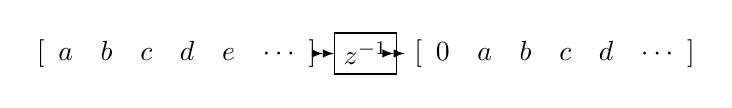
\begin{tikzpicture}[auto,>=latex,node distance=2.4cm]
    \node[] (input) {$\sv{a b c d e}$};
    \node[block, right of=input] (z) {$z^{-1}$};
    \node[right of=z] (output) {$\sv{0 a b c d}$};
    \draw[->>] (input) -- (z);
    \draw[->>] (z) -- (output);
  \end{tikzpicture}
\end{center}
\vspace{-1ex}
%\end{definition}
%
A very important property of the delay operator is that it produces
the first output \emph{before} having received the first input, and it
produces the second output before having received the second input,
etc.

%\begin{definition}[Time invariance]
%A stream operator $S: \stream{A} \to \stream{B}$ is \defined{time-invariant} (TI) if
%$S(\zm_A(s)) = \zm_B(S(s))$ for all $s \in \stream{A}$; in other words, if
%the following two circuits are equivalent:
%
%\begin{tabular}{m{3cm}m{.5cm}m{3cm}}
%\begin{tikzpicture}[auto,>=latex]
%  \node[] (input) {$s$};
%  \node[block, right of=input] (S) {$S$};
%  \node[block, right of=S] (z) {$\zm$};
%  \node[right of=z] (output) {$o$};
%  \draw[->] (input) -- (S);
%  \draw[->] (S) -- (z);
%  \draw[->] (z) -- (output);
%\end{tikzpicture}
%&
%$\cong$
%&
%\begin{tikzpicture}[auto,>=latex]
%  \node[] (input) {$s$};
%  \node[block, right of=input] (z) {$\zm$};
%  \node[block, right of=z] (S) {$S$};
%  \node[right of=S] (output) {$o$};
%  \draw[->] (input) -- (z);
%  \draw[->] (z) -- (S);
%  \draw[->] (S) -- (output);
%\end{tikzpicture}
%\end{tabular}
%
%\noindent
%This definition extends
%naturally to operators with multiple inputs.
%\end{definition}
%
%The composition of TI operators of any number of inputs
%is TI. The delay operator $\zm$ is TI.
%\dbsp only uses TI operators.
%
%%\begin{definition}
%%We say that a function between groups $f: A \to B$ has the \emph{zero-preservation
%%property} if $f(0_A) = 0_B$.  We write $\zpp{f}$.
%%\end{definition}
%%
%%A lifted operator $\lift{f}$ is TI iff $\zpp{f}$.
%
%\subsubsection{Causal and strict operators}\label{sec:causal}
%
%\begin{definition}[Causality]
%A stream operator $S:\stream{A}\to\stream{B}$
%is \defined{causal} when for all $s,s'\in\stream{A}$,
%and all times $t$ we have:
%$
%(\forall i \leq t . s[i]=s'[i]) ~~\Rightarrow~~ S(s)[t]=S(s')[t].
%$
%\end{definition}
%
%\noindent
%In other words, the output value at time $t$ can only depend on
%input values from times $t' \leq t$.
%Operators produced by lifting are causal, and $\zm$ is causal.
%All \dbsp operators are causal.  The composition
%of causal operators of any number of inputs is causal.
%
%\begin{definition}[Strictness]
%A stream operator, $F:\stream{A}\to\stream{B}$
%is \defined{strict}
%if  $\forall s,s'\in\stream{A}, \forall t \in \N$ we have:
%$(\forall i<t . ~s[i]=s'[i]) ~~\Rightarrow \\ F(s)[t]=F(s')[t].$
%\end{definition}
%
%In other words, the $t$-th output of $F(s)$ can depend only on ``past'' values
%of the input $s$, between $0$ and $t-1$.
%In particular, $F(s)[0] = 0_B$ is the same for all $s \in \stream{A}$.
%Strict operators are causal. Lifted operators in general are \emph{not} strict.
%$\zm$ is strict.  %In \dbsp $\zm$ is the only primitive strict operator.
%
%\begin{proposition}
%\label{prop-unique-fix}
%For a strict $F: \stream{A} \to \stream{A}$ the equation ~$\alpha=F(\alpha)$~ has a unique
%solution $\alpha \in \stream{A}$, denoted by $\fix{\alpha}{F(\alpha)}$.
%\end{proposition}
%
%Thus every strict operator from a set to itself has a unique fixed
%point.  The simple proof relies on strong induction, showing that the
%solution $\alpha[t]$ depends only on the values of $\alpha$ prior to
%$t$.
%
%Consider a circuit with a strict feedback edge:
%\begin{center}
%\begin{tikzpicture}[>=latex]
%    \node[] (input) {$s$};
%    \node[block, right of=input] (f) {$T$};
%    \node[right of=f] (output) {$\alpha$};
%    \node[block, below of=f, node distance=.5cm] (z) {$F$};
%    \draw[->] (input) -- (f);
%    \draw[->] (f) -- node (mid) {} (output);
%    \draw[->] (mid.center) |-  (z);
%    \draw[->] (z.west) -- ++(-.3,0) |- ([yshift=1mm]f.south west);
%\end{tikzpicture}
%\end{center}
%
%This circuit is a well-defined function on streams:
%
%%\begin{lemma}
%%\label{lemma-causal-strict}
%%If $F: \stream{B} \to \stream{B}$ is strict and $T: \stream{A} \times \stream{B} \to \stream{B}$ is causal, then for fixed $s$ the operator
%%$\lambda\alpha.T(s,F(\alpha)): \stream{A} \to \stream{B}$ is strict.
%%\end{lemma}
%
%\begin{lemma}\label{feedback-semantics}
%\label{cor-loop}
%If $F: \stream{B} \to \stream{B}$ is strict and $T: \stream{A} \times \stream{B} \to \stream{B}$ is causal,
%the operator $Q(s)=\fix{\alpha}{T(s,F(\alpha))}$ is well-defined and causal.
%If, moreover, $F$ and $T$ are TI then so is $Q$.
%\end{lemma}
%
%All \dbsp computations are built using just lifted functions and
%delays.  We add two more operators in \secref{sec:nested}.
%
%\subsection{Integration and differentiation}\label{sec:abelianstreams}

%Remember that we require the elements of a stream to come from an abelian group $A$.
%Streams themselves form an abelian group:
%
%\begin{proposition}
%The structure $(\stream{A},+,0,-)$, obtained by lifting the $+$ and unary $-$ operations of $A$,
%is an abelian group.  0 is the stream with all values $0_A$.
%\end{proposition}
%
%\noindent
%Stream addition and negation are causal, TI operators.

%Given a linear function $f: A \to B$, the stream operator $\lift{f}$
%is linear and TI (LTI).  $\zm$ is also LTI.
%
%\begin{definition}(bilinear)
%A function of two arguments $f: A \times B \to C$ with $A, B, C$ groups, is \emph{bilinear}
%if it is linear separately in each argument (i.e., it distributes over addition):
%$\forall a, b, c, d . f(a+b, c) = f(a, c) + f(b, c)$, and $f(a, c+d) = f(a, c) + f(c, d).$
%\end{definition}
%
%This definition extends to stream operators.
%The lifting of a bilinear function $f$ is
%a bilinear stream operator $\lift{f}$.  An example
%is lifted multiplication:
%$f: \stream{\N} \times \stream{\N} \to \stream{\N}, f(a, b)[t] = a[t]\cdot b[t]$.

%The composition of (bi)linear operators with linear operators
%is (bi)linear (since homomorphisms compose).

%The ``feedback loop'' of a linear operator is linear:
%
%\begin{proposition}
%\label{prop-rec-linear}
%Let $S$ be a unary, causal, LTI operator. The
%operator $Q(s)=\fix{\alpha}{S(s+\zm(\alpha))}$ is well-defined and LTI:
%
%\begin{center}
%\begin{tikzpicture}[>=latex]
%    \node[] (input) {$s$};
%    \node[block, shape=circle, right of=input, inner sep=0pt, node distance=.6cm] (plus) {$+$};
%    \node[block, right of=plus, node distance=.6cm] (Q) {$S$};
%    \node[right of=Q, node distance=1.2cm] (output) {$\alpha$};
%    \node[block, below of=Q, node distance=.6cm] (z) {$\zm$};
%    \draw[->] (input) -- (plus);
%    \draw[->] (plus) -- (Q);
%    \draw[->] (Q) -- node (mid) {} (output);
%    \draw[->] (mid.center) |-  (z);
%    \draw[->] (z) -| (plus);
%\end{tikzpicture}
%\end{center}
%\end{proposition}

%\begin{definition}[Differentiation]
We define the \defined{differentiation operator} as a composition of
several other operators: $\D(s) \defn s - \zm(s)$, shown as:
%
\vspace{-2ex}
\begin{center}
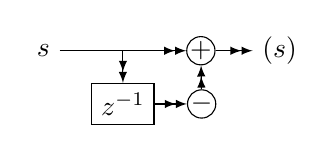
\begin{tikzpicture}[auto,>=latex,node distance=1cm]
    \node[] (input) {$s$};
    \node[block, shape=circle, right of=input, inner sep=0pt,node distance=2cm] (plus) {$+$};
    \node[right of=plus] (output) {$\D(s)$};
    \draw[->>] (input) -- node (i) {} (plus);
    \node[block, below of=i, node distance=.8cm] (z) {$\zm$};
    \node[block, shape=circle, right of=z, inner sep=0pt] (minus) {$-$};
    \draw[->>] (plus) -- (output);
    \draw[->>] (i) -- (z);
    \draw[->>] (z) -- (minus);
    \draw[->>] (minus) -- (plus);
\end{tikzpicture}
\end{center}
%\end{definition}
%We generally omit the type, and write just $\D$.
%The value of $\D(s)[t] = s[t] - s[t-1]$ if $t > 0$.
%
If $s$ is a stream, then $\D(s)$ is the \emph{stream of changes} of
$s$; a value in the output is the difference between two consecutive
values in the input.  As an example:
{
\noindent \small
\begin{align*}
  &\D(\sv{0 1 2 1 0}) &= \\
  &\sv{0 1 2 1 0} - \zm(\sv{0 1 2 1 0}) &=\\
  &\sv{0 1 2 1 0} - \sv{0 0 1 2 1} &=\\
%  &\sv{0-0 1-0 2-1 1-2 0-1} =\\
  &\sv{0 1 1 -1 -1}
\end{align*}
}

%\begin{proposition}
%\label{prop-diff-properties}
%$\D$ is causal and LTI.
%\end{proposition}

%The integration operator ``reconstitutes'' a stream from its changes:

%\begin{definition}[Integration]
The \defined{integration operator}
is given by the following circuit:
\vspace{-2ex}
\begin{center}
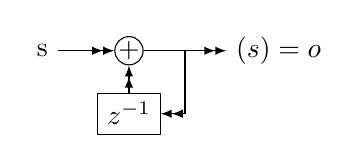
\begin{tikzpicture}[auto,>=latex, node distance=1.1cm]
    \node[] (input) {s};
    \node[block, shape=circle, right of=input, inner sep=0pt] (plus) {$+$};
    \node[right of=plus, node distance=1.9cm] (output) {$\I(s) = o$};
    \node[block, below of=plus, node distance=.8cm] (z) {$z^{-1}$};
    \draw[->>] (input) -- (plus);
    \draw[->>] (plus) -- node (o) {} (output);
    \draw[->>] (o) |- (z);
    \draw[->>] (z) -- (plus);
\end{tikzpicture}
\end{center}
\vspace{-1ex}
%\end{definition}
%
While this definition may seem strange, because the output stream is
used to compute itself, the use of the delay in the ``feedback'' loop
ensures that only \emph{previous} values of the output are used in
computing the current one.  Using the notation $o = \I(s)$ to make
formulas more readable, we can see the contents of stream $o$ is
produced step by step:
\begin{align*}
  o[0] &= s[0] + (\zm(o))[0] = s[0] + 0 = s[0] \\
  o[1] &= s[1] + (\zm(o))[1] = s[1] + o[0] = s[1] + s[0] \\
  o[2] &= s[2] + (\zm(o))[2] = s[2] + o[1] = s[2] + (s[1] + s[0])
\end{align*}

%\noindent
%We also generally omit the type, and write just $\I$.
%This is the construction from Proposition~\ref{prop-rec-linear}
%using the identity function for $S$.
%
%\begin{proposition}
%$\I(s)$ is the discrete (indefinite) integral applied to the stream $s$:
%\end{proposition}
In general, $\I(s)[t] = o[t] = \sum_{i \leq t} s[i]$.
Examples:
\begin{align*}
  \I(\sv{0 1 2 3 4 5}) &= \sv{0 1 3 6 10} \\
  \I(\sv{0 1 1 -1 -1}) &= \sv{0 1 2 1 0}.
\end{align*}

%\begin{proposition}
%\label{prop-integ-properties}
%$\I$ is causal and LTI.
%\end{proposition}
%
%\begin{theorem}[Inversion]
%\label{inverses}
%Integration and differentiation are inverses of each other:
%$\forall s . \I(\D(s)) = \D(\I(s)) = s$.
%\end{theorem}

Integration and differentiation are inverses of each other: while $\D$
computes the changes of a stream, $\I$ reconstitutes the original
stream given the stream of changes.  $\I$ and $\D$ ``cancel out'' when
applied in sequence:

\noindent
\begin{tabular}{m{2.5cm}m{.3cm}m{1cm}m{.3cm}m{2.5cm}}
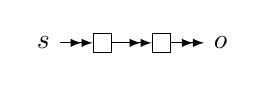
\begin{tikzpicture}[auto,>=latex, node distance=.75cm]
    \node[] (input) {$s$};
    \node[block, right of=input] (I) {$\I$};
    \node[block, right of=I] (D) {$\D$};
    \node[right of=D] (output) {$o$};
    \draw[->>] (input) -- (I);
    \draw[->>] (I) -- (D);
    \draw[->>] (D) -- (output);
\end{tikzpicture}
     &
     $\cong$
     &
     \hspace{-2ex}
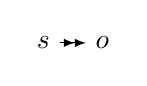
\begin{tikzpicture}[auto,>=latex, node distance=.75cm]
    \node[] (input) {$s$};
    \node[right of=input] (output) {$o$};
    \draw[->>] (input) -- (output);
\end{tikzpicture}
     &
     $\cong$
     &
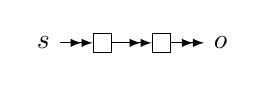
\begin{tikzpicture}[auto,>=latex, node distance=.75cm]
    \node[] (input) {$s$};
    \node[block, right of=input] (D) {$\D$};
    \node[block, right of=D] (I) {$\I$};
    \node[right of=I] (output) {$o$};
    \draw[->>] (input) -- (D);
    \draw[->>] (D) -- (I);
    \draw[->>] (I) -- (output);
\end{tikzpicture}
\end{tabular}

\section{Incremental view maintenance}\label{sec:incremental}

The results in this section are not specific to databases, they hold
for any stream computations, but we hint about their applicability for
databases.

%Here we define IVM and analyze its properties.

%\begin{definition}
Given a stream operator $S: \stream{A} \to \stream{B}$ we define the
\defined{incremental version} of $S$ as:
%\begin{equation}\label{def:inc}
%\inc{Q} \defn \D \circ Q \circ \I.
%\end{equation}
%$\inc{Q}$ has the same ``type'' as $Q$: $\inc{Q}: \stream{A} \to \stream{B}$.

%The following diagram illustrates the intuition behind this
%definition:
\vspace{-2ex}
\begin{center}
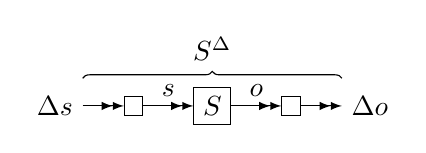
\begin{tikzpicture}[auto,>=latex]
    \node[] (input) {$\Delta s$};
    \node[block, right of=input] (I) {$\I$};
    \node[block, right of=I] (Q) {$S$};
    \node[block, right of=Q] (D) {$\D$};
    \node[right of=D] (output) {$\Delta o$};
    \draw[->>] (input) -- (I);
    \draw[->>] (I) -- node (s) {$s$} (Q);
    \draw[->>] (Q) -- node (o) {$o$} (D);
    \draw[->>] (D) -- (output);
    \draw[decorate, decoration = {brace, raise=10pt}] (input) -- (output)
    node[pos=.5, above=13pt]{$\inc{S}$};
\end{tikzpicture}
\end{center}
\vspace{-1ex}
%\end{definition}

If $S$ computes on a stream $s$, then $\inc{S}$ computes on a stream
of changes to $s$.  If $S$ produces a stream $o$, then $\inc{S}$
produces the stream of changes to $o$.  Note that this definition does
not require $S$ to be a lifted function.

For an operator with multiple inputs and outputs we define the
incremental version by applying $\I$ to each input, and $\D$ to each
output, e.g.: $\inc{T}(a, b) \defn \D (T(\I(a), \I(b)))$.

%Notice that our definition of incremental computation is meaningful only for \emph{streaming}
%computations; this is in contrast to classic definitions, e.g.~\cite{gupta-idb95} which
%consider only one change.  Generalizing the definition to operate on streams gives us
%additional power, especially when operating with recursive queries.
%
%The following proposition is one of our central results:
$\inc{S}$ has many nice properties:

%\begin{proposition}(Properties of the incremental version):
%\label{prop-inc-properties}
%\begin{description}
%\item[inversion:] $Q\mapsto\inc{Q}$ is bijective; its inverse is $Q\mapsto \I\circ Q\circ\D$.
%\item[invariance:] $\inc{+} = +, \inc{(\zm)} = \zm, \inc{-} = -, \inc{\I}=\I, \inc{\D}=\D$
%\item[push/pull:] \label{prop-part-commutation}
%    $Q \circ \I = \I \circ \inc{Q}$; $\D\circ Q = \inc{Q}\circ\D$
%\item[chain:] $\inc{(Q_1\circ Q_2)} = \inc{Q_1}\circ\inc{Q_2}$ (Generalizes to multiple inputs.)
%\item[add:] $\inc{(Q_1 + Q_2)} = \inc{Q_1} + \inc{Q_2}$
%\item[cycle:] $\inc{(\lambda s. \fix{\alpha}{T(s,\zm(\alpha)}))} = \lambda s. \fix{\alpha}{\inc{T}(s,\zm(\alpha)})$
%\end{description}
%\end{proposition}
%
The \defined{chain rule} states that $\inc{(Q_1 \circ Q_2)} =
\inc{Q_1} \circ \inc{Q_2}$, i.e., these circuits are equivalent:

\noindent
\begin{tabular}{cr}
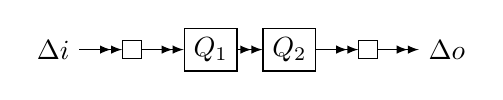
\begin{tikzpicture}[auto,>=latex]
  \node[] (input) {$\Delta i$};
  \node[block, right of=input] (I) {$\I$};
  \node[block, right of=I] (Q1) {$Q_1$};
  \node[block, right of=Q1] (Q2) {$Q_2$};
  \node[block, right of=Q2] (D) {$\D$};
  \node[right of=D] (output)  {$\Delta o$};
  \draw[->>] (input) -- (I);
  \draw[->>] (I) -- (Q1);
  \draw[->>] (Q1) -- (Q2);
  \draw[->>] (Q2) -- (D);
  \draw[->>] (D) -- (output);
\end{tikzpicture} &
$\cong$ \\
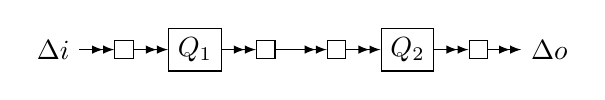
\begin{tikzpicture}[>=latex, node distance=.9cm]
  \node[] (input) {$\Delta i$};
  \node[block, right of=input] (I1) {$\I$};
  \node[block, right of=I1] (Q1) {$Q_1$};
  \node[block, right of=Q1] (D1) {$\D$};
  \node[block, right of=D1] (I2) {$\I$};
  \node[block, right of=I2] (Q2) {$Q_2$};
  \node[block, right of=Q2] (D2) {$\D$};
  \node[right of=D2] (output)  {$\Delta o$};
  \draw[->>] (input) -- (I1);
  \draw[->>] (I1) -- (Q1);
  \draw[->>] (Q1) -- (D1);
  \draw[->>] (D1) -- (I2);
  \draw[->>] (I2) -- (Q2);
  \draw[->>] (Q2) -- (D2);
  \draw[->>] (D2) -- (output);
\end{tikzpicture} &
$\cong$ \\
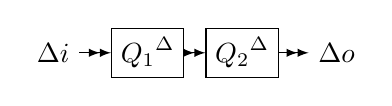
\begin{tikzpicture}[>=latex, node distance=1.2cm]
  \node[] (input) {$\Delta i$};
  \node[block, right of=input] (Q1) {$\inc{Q_1}$};
  \node[block, right of=Q1] (Q2) {$\inc{Q_2}$};
  \node[right of=Q2] (output)  {$\Delta o$};
  \draw[->>] (input) -- (Q1);
  \draw[->>] (Q1) -- (Q2);
  \draw[->>] (Q2) -- (output);
\end{tikzpicture}
\end{tabular}

\noindent In the database world, we can read this as: \textbf{to
  incrementalize a composite query you can incrementalize each
  sub-query independently}.  This gives us a simple deterministic
recipe reducing the incremental version of an arbitrary query to the
incremental version of its primitive operators.

The \defined{cycle rule} states that these circuits are equivalent:

\noindent
\begin{tabular}{m{4.4cm}m{.2cm}m{3cm}}
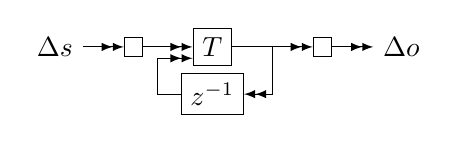
\begin{tikzpicture}[>=latex]
    \node[] (input) {$\Delta s$};
    \node[block, right of=input] (I) {$\I$};
    \node[block, right of=I] (f) {$T$};
    \node[block, right of=f, node distance=1.4cm] (D) {$\D$};
    \node[right of=D] (output) {$\Delta o$};
    \node[block, below of=f, node distance=.6cm] (z) {$\zm$};
    \draw[->>] (input) -- (I);
    \draw[->>] (I) -- (f);
    \draw[->>] (f) -- node (mid) {} (D);
    \draw[->>] (mid.center) |-  (z);
    \draw[->>] (z.west) -- ++(-.3,0) |- ([yshift=1mm]f.south west);
    \draw[->>] (D) -- (output);
\end{tikzpicture} & $\cong$ &
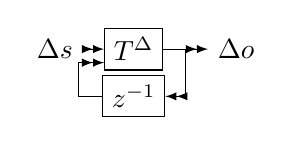
\begin{tikzpicture}[>=latex]
    \node[] (input) {$\Delta s$};
    \node[block, right of=input] (f) {$\inc{T}$};
    \node[right of=f, node distance=1.3cm] (output) {$\Delta o$};
    \node[block, below of=f, node distance=.6cm] (z) {$\zm$};
    \draw[->>] (input) -- (f);
    \draw[->>] (f) -- node (mid) {} (output);
    \draw[->>] (mid.center) |-  (z);
    \draw[->>] (z.west) -- ++(-.3,0) |- ([yshift=1mm]f.south west);
\end{tikzpicture}
\end{tabular}

\noindent
(We have omitted the labels on the inputs of $T$.) In other words, the
incremental version of a feedback loop around a query is just the
feedback loop with the incremental query for its body.  This result
will be useful for recursive queries.

%To execute incremental queries efficiently, we want to compute directly
%on streams of changes, without integrating them. The invariance property above shows
%that stream operators $+$, $-$, and $\zm$ are identical to their incremental versions.
%The following theorems generalize this to linear and bi-linear operators:

We call an operator $S$ \defined{linear} if it has the property that
$S(a+b) = S(a) + S(b)$ (where $+$ is the addition of streams).
%
%\begin{theorem}[Linear]\label{linear}
For a linear operator $S$ we have $\inc{S}=S$.
%\end{theorem}
%
This is very useful because many primitive database operations can be
implemented as linear operators: selection, projection, filtering,
grouping, parts of aggregation are all linear.  Moreover, the
following operators are linear: $-$, $z^{-1}$, $\I$, $\D$, $\lift{f}$
if $f$ is a linear function.

We call an operator $T$ with two inputs \defined{bilinear} if it
distributes over stream addition: $T(a+b, c) = T(a, c) + T(b, c)$, and
$T(a, c+d) = T(a, c) + T(a, d)$.  (Similar to multiplication's
distributivity over addition.)  In databases intersection, joins, and
Cartesian products are bilinear.

%\begin{theorem}[Bilinear]\label{bilinear}
Using infix notation, for a bilinear operator $\times$ we have:
\begin{eqnarray*}
\inc{(\Delta a \times \Delta b)} = \\
(\Delta a \times \Delta b ~+~ \zm(\I(\Delta a)) \times
\Delta b ~+~ \Delta a \times \zm(\I(\Delta b)) = \\
\Delta a \times \Delta b + \zm(a) \times \Delta b + \Delta a \times \zm(b)
\end{eqnarray*}

If we ignore the delay operators in this equation we recover the
well-known formula for join delta queries, e.g.,\cite{koch-pods10}.

%In pictures: \\
\noindent
\begin{tabular}{m{3.3cm}m{0cm}m{4cm}%m{0cm}m{2.8cm}
  }
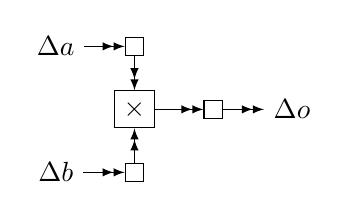
\begin{tikzpicture}[auto,>=latex]
    \node[] (a) {$\Delta a$};
    \node[block, right of=a] (ai) {$\I$};
    \node[below of=a, node distance=.8cm] (midway) {};
    \node[below of=midway, node distance=.8cm] (b) {$\Delta b$};
    \node[block, right of=b] (bi) {$\I$};
    \node[block, right of=midway, node distance=1cm] (q) {$\times$};
    \node[block, right of=q] (D) {$\D$};
    \node[right of=D] (output) {$\Delta o$};
    \draw[->>] (a) -- (ai);
    \draw[->>] (b) -- (bi);
    \draw[->>] (ai) -- (q);
    \draw[->>] (bi) -- (q);
    \draw[->>] (q) -- (D);
    \draw[->>] (D) -- (output);
\end{tikzpicture} &
$\cong$ &
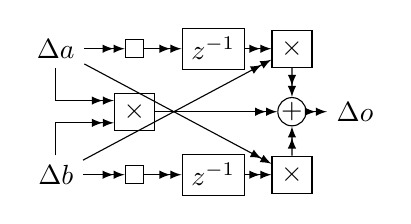
\begin{tikzpicture}[auto,>=latex]
  \node[] (input1) {$\Delta a$};
  \node[below of=input1, node distance=1.6cm] (input2) {$\Delta b$};
  \node[block, right of=input1, node distance=1cm] (I1) {$\I$};
  \node[block, below of=I1,node distance=.8cm] (ab) {$\times$};
  \node[block, right of=input2, node distance=1cm] (I2) {$\I$};
  \draw[->>] (input1) -- (I1);
  \draw[->>] (input2) -- (I2);
  \draw[->>] (input1) |- ([yshift=-1mm]ab.north west);
  \draw[->>] (input2) |- ([yshift=1mm]ab.south west);
  \node[block, right of=I1] (ZI1) {$\zm$};
  \node[block, right of=I2] (ZI2) {$\zm$};
  \draw[->>] (I1) -- (ZI1);
  \draw[->>] (I2) -- (ZI2);
  \node[block, right of=ZI1] (DI1) {$\times$};
  \node[block, right of=ZI2] (DI2) {$\times$};
  \draw[->>] (ZI1) -- (DI1);
  \draw[->>] (ZI2) -- (DI2);
  \node[block, circle, right of=ab, inner sep=0cm, node distance=2cm] (sum) {$+$};
  \draw[->>] (ab) -- (sum);
  \draw[->>] (DI1) -- (sum);
  \draw[->>] (DI2) -- (sum);
  \node[right of=sum, node distance=.8cm] (output) {$\Delta o$};
  \draw[->>] (sum) -- (output);
  \draw[->>] (input1) -- (DI2);
  \draw[->>] (input2) -- (DI1);
\end{tikzpicture}
%&
%$\cong$ &
%\begin{tikzpicture}[auto,>=latex,node distance=.7cm]
%  \node[] (input1) {$a$};
%  \node[below of=input1, node distance=1cm] (input2) {$b$};
%  \node[block, right of=input1, node distance=.5cm] (I1) {$\I$};
%  \node[block, right of=input2, node distance=.5cm] (I2) {$\I$};
%  \draw[->>] (input1) -- (I1);
%  \draw[->>] (input2) -- (I2);
%  \node[block, right of=I2] (ZI2) {$\zm$};
%  \draw[->>] (I2) -- (ZI2);
%  \node[block, right of=I1] (DI1) {$\times$};
%  \node[block, right of=ZI2] (DI2) {$\times$};
%  \draw[->>] (I1) -- (DI1);
%  \draw[->>] (ZI2) -- (DI2);
%  \node[block, circle, above of=DI2, inner sep=0cm, node distance=.5cm] (sum) {$+$};
%  \draw[->>] (DI1) -- (sum);
%  \draw[->>] (DI2) -- (sum);
%  \node[right of=sum, node distance=.5cm] (output) {$o$};
%  \draw[->>] (sum) -- (output);
%  \draw[->>] (input1) -- (DI2);
%  \draw[->>] (input2) -- (DI1);
%\end{tikzpicture}
\end{tabular}
%\end{theorem}

What is the intuition behind this diagram?  Let us consider the case
of Cartesian product $a \times b$.  The incremental product has inputs
$\Delta a = \D(a)$ and $\Delta b = \D(b)$.  What happens when we add a
row $x$ to relation $a$ (i.e., $\Delta a = x$)?  The new row $x$ will
appear in the output change combined with every row in the
\emph{previous version} of the \emph{full} relation $b$.  The operator
$\I(\Delta b)$ in fact computes relation $b$ from the stream $\Delta
b$ of changes, and $\zm$ applied to this value gives us its previous
version.  So the bottom $\times$ operator computes $x \times \zm(b) =
\Delta a \times \zm(\I(\Delta b))$, the change produced by the new row
$x$.  The top $\times$ operator performs the symmetric operation for
the changes of the $b$ relation.  The middle $\times$ operator
produces the results of changes to both inputs.

%Rewriting this statement using $\Delta a$ for the stream of changes to
%$a$ we get the familiar formula for incremental equi-joins:
%$\Delta(a\times b) =\Delta a \times \Delta b + a\times(\Delta b) +
%(\Delta a)\times b$; equi-joins are indeed bilinear.
%

\section{IVM for the Relational Algebra}\label{sec:relational}

Results in \secref{sec:streams} and~\secref{sec:incremental}
apply to streams of arbitrary group values.  In this
section we apply these results to
IVM for relational databases.  As explained in the introduction, our goal is to
efficiently compute the incremental version of any relational query $Q$
that defines a database view.

However, we face a technical problem: the $\I$ and $\D$ operators were
defined on abelian groups, and relational databases in general are
not abelian groups, since they operate on sets.  Fortunately,
there is a well-known tool in the database literature
which converts set operations into group operations by using \zrs
(also called z-relations~\cite{green-tcs11}) to represent sets.

We start by defining the \zrs group, and then we review how
relational queries are converted into \dbsp circuits  over \zrs.
This translation is efficiently incrementalizable because
many basic relational queries can be expressed using LTI \zr operators~\refsec{sec:relational-operators}.

\subsection{\zrs as an abelian group}

\zrs generalize database tables: think of a \zr as a table where each
row has an associated weight, possibly negative.

Given a set $A$, we define \defined{\zrs} over $A$ as functions with
\emph{finite support} from $A$ to $\Z$.  These are functions $f: A
\rightarrow \Z$ where $f(x) \not= 0$ for at most a finite number of
values $x \in A$.  We also write $\Z[A]$ for the type of \zrs with
elements from $A$.  Values in $\Z[A]$ can be thought of as key-value
maps with keys in $A$ and values in $\Z$, justifying the array
indexing notation.  If $m \in \Z[A]$ we write $m[a]$ instead of
$m(a)$, again using an indexing notation.

A particular \zr $m \in \Z[A]$ can be denoted by enumerating its
elements that have non-zero weights and their corresponding weights:
$m = \{ x_1 \mapsto w_1, \dots, x_n \mapsto w_n \}$.
We call $w_i \in \Z$ the \defined{weight}
of $x_i \in A$.  Weights can be negative.
We write that $x \in m$ iff $m[x] \not= 0$.
We also write $w \cdot x$ for $\{ x \mapsto w \}$.

\ifzsetexamples
Consider a concrete \zr $R \in \Z[\texttt{string}]$,
defined by $R = \{ \texttt{joe} \mapsto 1, \texttt{anne} \mapsto -1 \}$.
$R$ has two elements in its domain,
\texttt{joe} with weight 1 (so $R[\texttt{joe}] = 1$),
and \texttt{anne} with weight $-1$.
We say \texttt{joe} $\in R$ and \texttt{anne} $\in R$.
\fi

Since $\Z$ is an abelian ring, $\Z[A]$ is also an abelian ring (and thus a group).  This group
$(\Z[A], +_{\Z[A]}, 0_{\Z[A]}, -_{\Z{A}})$ has addition and subtraction defined pointwise:
$(f +_{\Z[A]} g)(x) = f(x) + g(x) . \forall x \in A.$
The $0$ element of $\Z[A]$ is the function $0_{\Z[A]}$ defined by $0_{\Z[A]}(x) = 0 .
\forall x \in A$.  For example, $R + R =  \{ \texttt{joe} \mapsto 2, \texttt{anne} \mapsto -2 \}$.
Since \zrs form a group, all results from \secref{sec:streams} apply to streams over \zrs.

\zrs generalize sets and bags.  A set with elements from $A$
can be represented as a \zr by associating a weight of 1 with each element.
Bags are \zrs where all weights are positive.  Crucially, \zrs
can also represent arbitrary \emph{changes} to sets and bags.
Negative weights in a change represent elements that are being ``removed''.

\begin{definition}
We say that a \zr represents a \defined{set} if the weight of every
element is one.  We define a function to check this property
$\isset : \Z[A] \rightarrow \B$\index{isset}
given by:
$$\isset(m) \defn \left\{
\begin{array}{ll}
  \mbox{true} & \mbox{ if } m[x] = 1, \forall x \in m \\
  \mbox{false} & \mbox{ otherwise}
\end{array}
\right.
$$
\end{definition}

\ifzsetexamples
For our example $\isset(R) = \mbox{false}$, since $R[\texttt{anne}] = -1$.
\fi

\begin{definition}
We say that a \zr is \defined{positive} (or a \defined{bag}) if the weight of every element is
positive.  We define a function to check this property
$\ispositive : \Z[A] \rightarrow \B$\index{ispositive}.
given by
$$\ispositive(m) \defn \left\{
\begin{array}{ll}
  \mbox{true} & \mbox{ if } m[x] \geq 0, \forall x \in A \\
  \mbox{false} & \mbox{ otherwise}
\end{array}
\right.$$
\end{definition}
We have $\forall m \in \Z[A] . \isset(m) \Rightarrow \ispositive(m)$.
\ifzsetexamples
$\ispositive(R) = \mbox{false}$, since $R[\texttt{anne}] = -1$.
\fi

We write $m \geq 0$ when $m$ is positive.  For positive $m, n \in
\Z[A]$ we write $m \geq n$ for iff $m - n \geq 0$.  $\geq$ is a
partial order.

We call a function $f : \Z[A] \rightarrow \Z[B]$ \defined{positive} if it maps
positive values to positive values:
$\forall x \in \Z[A], x \geq 0_{\Z[A]} \Rightarrow f(x) \geq 0_{\Z[B]}$.
We use the same notation for functions: $\ispositive(f)$.

\begin{definition}[distinct]
The function $\distinct: \Z[A] \rightarrow \Z[A]$\index{distinct}
``converts'' a \zr into a set:
$$\distinct(m)[x] \defn \left\{
\begin{array}{ll}
  1 & \mbox{ if } m[x] > 0 \\
  0 & \mbox{ otherwise}
\end{array}
\right.
$$
\end{definition}

Notice that $\distinct$ ``removes'' duplicates from multisets, and it also eliminates
elements with negative weights.
\ifzsetexamples
$\distinct(R) = \{ \texttt{joe} \mapsto 1 \}$.
\fi
While very simple, this definition of $\distinct$ has been carefully
chosen to enable us to implement the relational (set) operators
using \zrs operators.
%Circuits derived from relational queries only compute on positive \zrs.

%\begin{definition}(mononotonicity)
%A stream $s \in \stream{\Z[A]}$ is \defined{positive} if every value of the stream is positive:
%$s[t] \geq 0 . \forall t \in \N$.
%A stream $s \in \stream{\Z[A]}$ is \defined{monotone} if $s[t] \geq s[t-1], \forall t \in \N$.
%\end{definition}
%
%If $s \in \stream{\Z[A]}$ is positive, then $\I(s)$ is monotone.
%If $s \in \stream{\Z[A]}$ is monotone, $\D(s)$ is positive.
%
\paragraph{Generalizing circuit diagrams}

From now on we will use circuits to compute both on scalars (\zrs in our case) and streams of \zrs.
We use the same graphical representation for functions on streams or scalars:
boxes with input and output arrows.  For scalar functions the ``values''
of the arrows are scalars instead of streams; otherwise
the interpretation of boxes as function application is unchanged.  We will
thus use circuits to depict relational query plans.

\subsection{Implementing relational operators}\label{sec:relational-operators}

The fact that relational algebra can be implemented by computations
on \zrs has been shown before, e.g.~\cite{green-pods07}.  The translation
of the relational operators to \dbsp is shown in Table~\ref{tab:relational}.
The first row of the table shows that a composite query is translated
recursively.  This gives us a recipe for
translating an arbitrary relational query plan into a \dbsp circuit.

\newlength{\commentsize}
\setlength{\commentsize}{5cm}
\begin{table*}[h]
\small
\caption{Implementation of SQL relational set operators in \dbsp.
Each query assumes that inputs \code{I}, \code{I1}, \code{I2}, are sets and it
produces output sets.\label{tab:relational}}
\begin{tabular}{|m{1.2cm}m{4.2cm}m{5cm}m{\commentsize}|} \hline
Operation & SQL example & \dbsp circuit & Details \\ \hline
Composition &
 \begin{lstlisting}[language=SQL]
SELECT DISTINCT ... FROM
(SELECT ... FROM ...)
\end{lstlisting}
 &
 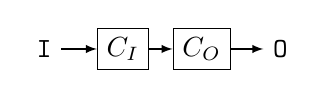
\begin{tikzpicture}[auto,>=latex]
  \node[] (I) {\code{I}};
  \node[block, right of=I] (CI) {$C_I$};
  \draw[->] (I) -- (CI);
  \node[block, right of=CI] (CO) {$C_O$};
  \node[right of=CO] (O) {\code{O}};
  \draw[->] (CI) -- (CO);
  \draw[->] (CO) -- (O);
\end{tikzpicture}
 &
 \parbox[b][][t]{\commentsize}{
  $C_I$ circuit for inner query, \\
  $C_O$ circuit for outer query.}
\\ \hline
Union &
\begin{lstlisting}[language=SQL]
(SELECT * FROM I1)
UNION
(SELECT * FROM I2)
\end{lstlisting}
&
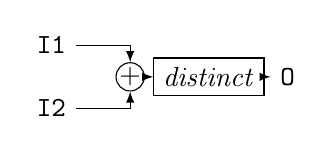
\begin{tikzpicture}[auto,>=latex]
  \node[] (input1) {\code{I1}};
  \node[below of=input1, node distance=.4cm] (midway) {};
  \node[below of=midway, node distance=.4cm] (input2) {\code{I2}};
  \node[block, shape=circle, right of=midway, inner sep=0in] (plus) {$+$};
  \node[block, right of=plus] (distinct) {$\distinct$};
  \node[right of=distinct] (output) {\code{O}};
  \draw[->] (input1) -| (plus);
  \draw[->] (input2) -| (plus);
  \draw[->] (plus) -- (distinct);
  \draw[->] (distinct) -- (output);
\end{tikzpicture}
& $\distinct$ eliminates duplicates.  An implementation of
\texttt{UNION ALL} does not need the $\distinct$.
\\ \hline
Projection &
\begin{lstlisting}[language=SQL]
SELECT DISTINCT I.c
FROM I
\end{lstlisting}
&
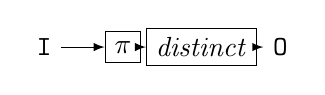
\begin{tikzpicture}[auto,>=latex]
  \node[] (input) {\code{I}};
  \node[block, right of=input] (pi) {$\pi$};
  \node[block, right of=pi] (distinct) {$\distinct$};
  \node[right of=distinct] (output) {\code{O}};
  \draw[->] (input) -- (pi);
  \draw[->] (pi) -- (distinct);
  \draw[->] (distinct) -- (output);
\end{tikzpicture}
&
\parbox[b][][t]{\commentsize}{
$\pi(i)[y] \defn
\sum_{x \in i, x|_c = y} i[x]$ \\
$x|_c$ is projection on column $c$ of the tuple $x$ \\
$\pi$ is linear; $\ispositive(\pi)$ %, \zpp{\pi}$.
}
\\ \hline
Filtering &
\begin{lstlisting}[language=SQL]
SELECT * FROM I
WHERE p(I.c)
\end{lstlisting}
&
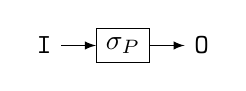
\begin{tikzpicture}[auto,>=latex]
  \node[] (input) {\code{I}};
  \node[block, right of=input] (map) {$\sigma_P$};
  \node[right of=map] (output) {\code{O}};
  \draw[->] (input) -- (map);
  \draw[->] (map) -- (output);
\end{tikzpicture}
&
\parbox[b][][t]{\commentsize}{
$\sigma_P(m)[x] \defn \left\{
\begin{array}{ll}
  m[x] & \mbox{ if } P(x) \\
  0 & \mbox{ otherwise } \\
\end{array}
\right.$ \\
$P: A \rightarrow \B$ is a predicate. \\
$\sigma_P$ is linear; $\ispositive(\sigma_P)$ % \zpp{\sigma_P}$.
}
% \\ \hline
%Selection &
%\begin{lstlisting}[language=SQL]
%SELECT DISTINCT f(I.c, ...)
%FROM I
%\end{lstlisting}
%&
%\begin{tikzpicture}[auto,>=latex]
%  \node[] (input) {\code{I}};
%  \node[block, right of=input, node distance=1.5cm] (map) {$\mbox{map}(f)$};
%  \node[block, right of=map, node distance=1.5cm] (distinct) {$\distinct$};
%  \node[right of=distinct, node distance=1.5cm] (output) {\code{O}};
%  \draw[->] (input) -- (map);
%  \draw[->] (map) -- (distinct);
%  \draw[->] (distinct) -- (output);
%\end{tikzpicture}
%&
%\parbox[b][][t]{\commentsize}{
%For a function $f$ \\
%$\map(f)$ is linear, \\
%$\ispositive(\map(f)), \zpp{\map(f)}$
%}.
\\ \hline
\parbox[b][][t]{1cm}{
Cartesian \\
product} &
\begin{lstlisting}[language=SQL]
SELECT I1.*, I2.*
FROM I1, I2
\end{lstlisting}
&
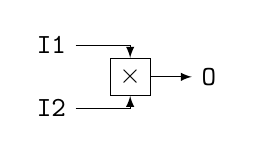
\begin{tikzpicture}[auto,>=latex]
  \node[] (i1) {\code{I1}};
  \node[below of=i1, node distance=.4cm] (midway) {};
  \node[below of=midway, node distance=.4cm] (i2) {\code{I2}};
  \node[block, right of=midway] (prod) {$\times$};
  \node[right of=prod] (output) {\code{O}};
  \draw[->] (i1) -| (prod);
  \draw[->] (i2) -| (prod);
  \draw[->] (prod) -- (output);
\end{tikzpicture}
&
\parbox[b][][t]{\commentsize}{
$(a \times b)((x,y)) \defn a[x] \times b[y]$. \\
$\times$ is bilinear, $\ispositive(\times)$ % , \zpp{\times}$.
}
\\ \hline
Equi-join &
\begin{lstlisting}[language=SQL]
SELECT I1.*, I2.*
FROM I1 JOIN I2
ON I1.c1 = I2.c2
\end{lstlisting}
&
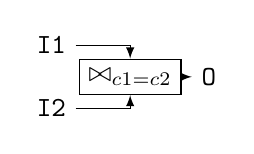
\begin{tikzpicture}[auto,>=latex]
  \node[] (i1) {\code{I1}};
  \node[below of=i1, node distance=.4cm] (midway) {};
  \node[below of=midway, node distance=.4cm] (i2) {\code{I2}};
  \node[block, right of=midway] (prod) {$\bowtie_{c1 = c2}$};
  \node[right of=prod] (output) {\code{O}};
  \draw[->] (i1) -| (prod);
  \draw[->] (i2) -| (prod);
  \draw[->] (prod) -- (output);
\end{tikzpicture}
&
\parbox[b][][t]{\commentsize}{
$(a \bowtie b)((x,y)) \defn a[x] \times b[y] \\
\mbox{ if } x|_{c1} = y|_{c2}$. \\
$\bowtie$ is bilinear, $\ispositive(\bowtie)$ %, \zpp{\bowtie}$.
}
\\ \hline
Intersection &
\begin{lstlisting}[language=SQL]
(SELECT * FROM I1)
INTERSECT
(SELECT * FROM I2)
\end{lstlisting}
&
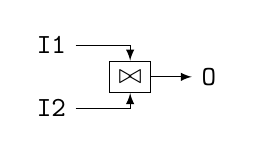
\begin{tikzpicture}[auto,>=latex]
  \node[] (i1) {\code{I1}};
  \node[below of=i1, node distance=.4cm] (midway) {};
  \node[below of=midway, node distance=.4cm] (i2) {\code{I2}};
  \node[block, right of=midway] (prod) {$\bowtie$};
  \node[right of=prod] (output) {\code{O}};
  \draw[->] (i1) -| (prod);
  \draw[->] (i2) -| (prod);
  \draw[->] (prod) -- (output);
\end{tikzpicture}
&
Special case of equi-join when both relations have the same schema.
 \\ \hline
Difference &
\begin{lstlisting}[language=SQL]
SELECT * FROM I1
EXCEPT
SELECT * FROM I2
\end{lstlisting}
&
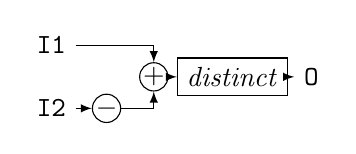
\begin{tikzpicture}[auto,>=latex, node distance=.7cm]
  \node[] (i1) {\code{I1}};
  \node[below of=i1, node distance=.4cm] (midway) {};
  \node[below of=midway, node distance=.4cm] (i2) {\code{I2}};
  \node[block, shape=circle, inner sep=0in, right of=i2] (m) {$-$};
  \node[block, right of=midway, shape=circle, inner sep=0in, node distance=1.3cm] (plus) {$+$};
  \node[block, right of=plus, node distance=1cm] (distinct) {$\distinct$};
  \node[right of=distinct, node distance=1cm] (output) {\code{O}};
  \draw[->] (i1) -| (plus);
  \draw[->] (i2) -- (m);
  \draw[->] (m) -| (plus);
  \draw[->] (plus) -- (distinct);
  \draw[->] (distinct) -- (output);
\end{tikzpicture}
&
$\distinct$ removes elements with negative weights from the result.
\\ \hline
\end{tabular}
\end{table*}


The translation is fairly straightforward, but many operators require
the application of a $\distinct$ \textbf{to produce sets}.
For example, $a \cup b = \distinct(a + b)$, $a \setminus b =
\distinct(a - b)$, $(a \times b)((x,y)) = a[x] \times b[y]$.
%\paragraph{Correctness of the \dbsp implementations}\label{sec:correctness}
%
%A relational query $Q$ that transforms
%a set $V$ into a set $U$ is implemented by a \dbsp computation $Q'$ on
%\zrs.  The correctness of the implementation requires the following
%diagram to commute:
%
%\begin{center}
%\begin{tikzpicture}
%  \node[] (V) {$V$};
%  \node[below of=V] (VZ) {$VZ$};
%  \node[right of=V, node distance=2cm] (U) {$U$};
%  \node[below of=U] (UZ) {$UZ$};
%  \draw[->] (V) -- node (f) [below] {$Q$} (U);
%  \draw[->] (V) --  node (s) [left] {tozset}(VZ);
%  \draw[->] (VZ) -- node (f) [above] {$Q'$} (UZ);
%  \draw[->] (UZ) -- node (d) [right] {toset} (U);
%\end{tikzpicture}
%\end{center}
%
%(The correctness of
%this implementation is predicated on $Q'$'s inputs being
%sets, an invariant which needs to be maintained by the environment.)
%The ``$\mbox{toset}$'' and ``$\mbox{tozset}$'' functions convert sets to \zrs and
%vice-versa, in the expected way:
%
%$\mbox{toset}: \Z[A] \to 2^A$ is defined as $\mbox{toset}(m) \defn \cup_{x \in \distinct(m)} \{ x \}$.
%
%$\mbox{tozset}: 2^A \to \Z[A]$ is defined as $\mbox{tozset}(s) \defn \sum_{x \in s} 1 \cdot x$.
%
%All standard algebraic properties
%of the relational operators can be used to optimize circuits
%(they can even be applied to queries before building the circuits).
%
Notice that the use of the $\distinct$ operator allows \dbsp to model
the \emph{full relational algebra}, including set difference (and not
just the positive fragment).

Prior work (e.g., Proposition 6.13 in~\cite{green-tcs11}) has shown
how some invocations of $\distinct$ can be eliminated from query plans
without changing the query semantics; we will see that incremental
versions of $\distinct$ operators incur significant space costs.

\begin{proposition}\label{prop-distinct-delay}
Let $Q$ be one of the following \zrs operators: filtering $\sigma$,
join $\bowtie$, or Cartesian product $\times$.
Then we have $\forall i \in \Z[I], \ispositive(i) \Rightarrow Q(\distinct(i)) = \distinct(Q(i))$.
\end{proposition}

\begin{comment}
\noindent
\begin{tabular}{m{3.5cm}m{.5cm}m{3.5cm}}
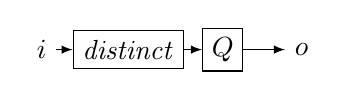
\begin{tikzpicture}[auto,>=latex]
  \node[] (input) {$i$};
  \node[block, right of=input, node distance=1.1cm] (distinct) {$\distinct$};
  \node[block, right of=distinct, node distance=1.2cm] (q) {$Q$};
  \node[right of=q] (output)  {$o$};
  \draw[->] (input) -- (distinct);
  \draw[->] (distinct) -- (q);
  \draw[->] (q) -- (output);
\end{tikzpicture}
&
$\cong$
&
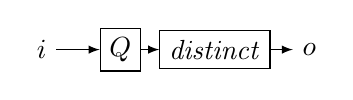
\begin{tikzpicture}[auto,>=latex]
  \node[] (input) {$i$};
  \node[block, right of=input] (q) {$Q$};
  \node[block, right of=q, node distance=1.2cm] (distinct1) {$\distinct$};
  \node[right of=distinct1, node distance=1.2cm] (output)  {$o$};
  \draw[->] (input) -- (q);
  \draw[->] (q) -- (distinct1);
  \draw[->] (distinct1) -- (output);
\end{tikzpicture}
\end{tabular}

This rule allows us to delay the application of $\distinct$.
\end{comment}

\begin{proposition}\label{prop-distinct-once}
Let $Q$ be one of the following \zrs operators: filtering $\sigma$,
projection $\pi$, map($f$)\footnote{Technically, map (applying a user-defined
function to each row) is not relational.},
addition $+$, join $\bowtie$, or
Cartesian product $\times$.
Then we have $\ispositive(i) \Rightarrow \distinct(Q(\distinct(i))) = \distinct(Q(i))$.
\end{proposition}

\begin{comment}
\noindent
\begin{tabular}{m{6.5cm}m{.5cm}}
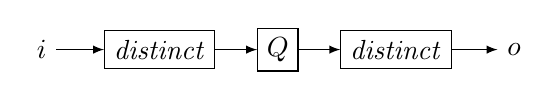
\begin{tikzpicture}[auto,>=latex]
  \node[] (input) {$i$};
  \node[block, right of=input, node distance=1.5cm] (distinct) {$\distinct$};
  \node[block, right of=distinct, node distance=1.5cm] (q) {$Q$};
  \node[block, right of=q, node distance=1.5cm] (distinct1) {$\distinct$};
  \node[right of=distinct1, node distance=1.5cm] (output)  {$o$};
  \draw[->] (input) -- (distinct);
  \draw[->] (distinct) -- (q);
  \draw[->] (q) -- (distinct1);
  \draw[->] (distinct1) -- (output);
\end{tikzpicture}
&
$\cong$ \\
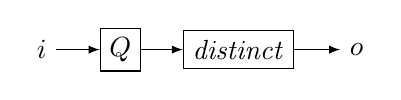
\begin{tikzpicture}[auto,>=latex]
  \node[] (input) {$i$};
  \node[block, right of=input] (q) {$Q$};
  \node[block, right of=q, node distance=1.5cm] (distinct1) {$\distinct$};
  \node[right of=distinct1, node distance=1.5cm] (output)  {$o$};
  \draw[->] (input) -- (q);
  \draw[->] (q) -- (distinct1);
  \draw[->] (distinct1) -- (output);
\end{tikzpicture}
\end{tabular}
\end{comment}

These properties allow us to ``consolidate'' distinct operators by performing
one $\distinct$ at the end of a chain of computations.

\subsection{Incremental view maintenance}

Let us consider a relational query $Q$ defining a view $V$.  To create
a circuit that maintains incrementally $V$ we apply the following
mechanical steps:

\begin{algorithm}[incremental view maintenance]\label{algorithm-inc}\quad
\begin{enumerate}[nosep, leftmargin=\parindent]
    \item Translate $Q$ into a circuit using the rules in Table~\ref{tab:relational}.
    \item Apply $\distinct$ elimination rules (\ref{prop-distinct-delay}, \ref{prop-distinct-once}) until convergence\footnote{The
    order in which the rules are applied does not matter, since the algorithm is
    confluent: it always produces the same final result.}.
    \item Lift the whole circuit, by applying Proposition~\ref{prop:distributivity},
    converting it to a circuit operating on streams.
    \item Incrementalize the whole circuit ``surrounding'' it with $\I$ and $\D$.
    \item Apply the chain rule
    from Proposition~\ref{prop-inc-properties} recursively on the query structure
    to obtain an incremental implementation.
\end{enumerate}
\end{algorithm}

This algorithm is deterministic and its running time
is proportional to the number of operators in the query.
Step (2) generates an equivalent circuit, with possibly fewer
$\distinct$ operators.  Step (3) yields a circuit that consumes a
\emph{stream} of complete database snapshots and outputs a stream of
complete view snapshots. Step (4) yields a circuit that consumes a
stream of \emph{database changes} and outputs a stream of \emph{view
changes}; however, the internal operation of the circuit is
non-incremental, as it rebuilds the complete database using
integration operators.  Step (5) incrementalizes the circuit by
replacing each primitive operator with its incremental version.

Most of the operators that appear in the circuits in
Table~\ref{tab:relational} are linear, and thus have very efficient
incremental versions (we discuss complexity in
\refsec{sec:complexity}).  A notable exception is $\distinct$.  The
next proposition shows that the incremental version of $\distinct$ is
also efficient, and it can be computed by doing work proportional to
the size of the input change:

\begin{proposition}\label{prop-inc_distinct}
The following circuit implements $\inc{(\lift{\distinct})}$:
\begin{tabular}{m{3.5cm}m{.0cm}m{5cm}}
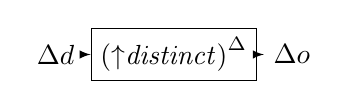
\begin{tikzpicture}[auto,node distance=1.5cm,>=latex]
    \node[] (input) {$\Delta d$};
    \node[block, right of=input] (d) {$\inc{(\lift{\distinct})}$};
    \node[right of=d] (output) {$\Delta o$};
    \draw[->] (input) -- (d);
    \draw[->] (d) -- (output);
\end{tikzpicture} &
$\cong$ &
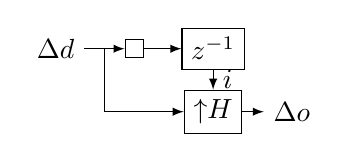
\begin{tikzpicture}[>=latex]
    \node[] (input) {$\Delta d$};
    \node[block, right of=input] (I) {$\I$};
    \node[block, right of=I] (z) {$\zm$};
    \node[block, below of=z, node distance=.8cm] (H) {$\lift{H}$};
    \node[right of=H] (output) {$\Delta o$};
    \draw[->] (input) -- node (mid) {} (I);
    \draw[->] (I) -- (z);
    \draw[->] (mid.center) |- (H);
    \draw[->] (z) -- node (i) [right] {$i$} (H);
    \draw[->] (H) -- (output);
\end{tikzpicture}
\end{tabular}

\noindent where $H: \Z[A] \times \Z[A] \to \Z[A]$ is defined as: \\
$$
H(i, d)[x] \defn
\begin{cases}
-1 & \mbox{if } i[x] > 0 \mbox{ and } (i + d)[x] \leq 0 \\
1  & \mbox{if } i[x] \leq 0 \mbox{ and } (i + d)[x] > 0 \\
0  & \mbox{otherwise} \\
\end{cases}
$$
\end{proposition}

Here is the intuition why $\distinct$ is efficiently
incrementalizable: the only elements that can appear in the output of
$\inc{(\lift{\distinct})}$ must have changed in the input.  So the
size of the output change cannot be bigger than the size of the input
change.  In the diagram above, $i$ is the previous version of the
integral of all changes, i.e., the full \zr whose $\distinct$ value is
being computed.  The function $H$ detects whether the weight of
an element in $i$ is changing sign (positive to negative or
vice-versa) when adding a new delta $d$.

%\refsec{sec:relational-example} shows a concrete example of a relational query converted
%into a circuit and then incrementalized using Algorithm~\ref{algorithm-inc}.

\subsection{Complexity of incremental circuits}\label{sec:complexity}

Incremental circuits are efficient.  We evaluate the cost of a circuit
while processing the $t$-th input change.  Even if $Q$ is a pure
function, $\inc{Q}$ is actually a streaming system, with internal
state.  This state is stored entirely in the delay operators $\zm$,
some of which appear in $\I$ and $\D$ operators.  The result produced
by $\inc{Q}$ on the $t$-th input depends in general not only on the
new $t$-th input, but also on all prior inputs it has received.

We argue that each operator in the incremental version of a circuit is
efficient in terms of work and space.  We make the standard IVM
assumption that the input changes \emph{of each operator} are small:
$|\Delta DB[t]| \ll |DB[t]| = |(\I(\Delta DB))[t]|$.

An unoptimized incremental operator $\inc{Q} = \D \circ Q \circ \I$
evaluates query $Q$ on the whole database $DB$, the integral of the input stream:
$DB = \I(\Delta DB)$; hence its time complexity  is the same as that of the non-incremental
evaluation of $Q$.  In addition, each of the $\I$ and $\D$ operators uses $O(|DB[t]|)$ memory.

Step (5) of the incrementalization algorithm applies the optimizations described in \secref{sec:incremental};
these reduce the time complexity of each operator to be a function of $O(|\Delta DB[t]|)$.
For example, Theorem~\ref{linear}, allows evaluating $\inc{S}$, where $S$ is a
linear operator, in time $O(|\Delta DB[t]|)$.  The $\I$
operator can also be evaluated in $O(|\Delta DB[t]|)$ time, because
all values that appear in the output of $\I(\Delta DB)[t]$ must be present in
current input change $\Delta DB[t]$.  Similarly, while the $\distinct$ operator is not
linear, $\inc{(\lift{\distinct})}$ can also be evaluated in $O(|\Delta DB[t]|)$ according to
Proposition~\ref{prop-inc_distinct}.  Bilinear operators, including join, can be
evaluated in time $O(|DB[t]| \times |\Delta DB[t]|)$, which is a factor of $|DB[t] / \Delta DB[t]|$
better than full re-evaluation.

The space complexity of linear operators is 0 (zero), since they store no
data persistently.  The space complexity of operators such as $\inc{(\lift{\distinct})}$,
$\inc{(\lift{\bowtie})}$, $\I$, and $\D$ is $O(|DB[t]|)$.  They need
to store their input or output relations in full.

\subsubsection{IVM query plans and optimality}

Let us look again at what we achieved using
Algorithm~\ref{algorithm-inc}.  A relational algebra query can be
implemented by multiple plans, each with a different data-dependent
cost\footnote{The optimal plan depends not only on the query, but also
  on the data.}.  The input of Algorithm~\ref{algorithm-inc} is a
(relational), non-incremental query plan, produced by a query planner.
The algorithm produces an incremental plan that is ``similar'' to the
input plan.

Standard query planners use cost-based heuristics and data statistics
to optimize plans.  A generic IVM planner does not have this luxury,
since the plan must be generated \emph{before} any data has been fed
to the database.  Nevertheless, all standard query optimization
techniques, perhaps based on historical statistics, can be used to
generate the query plan that is supplied to
Algorithm~\ref{algorithm-inc}.  The question of optimality in the
context of IVM plan is a much more difficult topic than optimization
of ad-hoc queries, since the chosen IVM plan will execute for
\emph{all future database updates}.

Moreover, since incremental computations maintain internal state, it
follows that incremental plans cannot be simply changed in-flight,
like we can change ad-hoc queries based on current data statistics:
deploying a new plan requires in general constructing its internal
state, which is produced by entire history of prior updates.
Fortunately, there is a trivial, but somewhat expensive, recipe for
installing a new incremental plan: feed the entire current state of
the database, as one big change.

\subsection{Relational Query Example}\label{sec:relational-example}

We apply the IVM algorithm~\ref{algorithm-inc} to a concrete
relational SQL query:
\begin{lstlisting}[language=SQL,basicstyle=\small]
CREATE VIEW v AS
SELECT DISTINCT a.x, b.y FROM (
     SELECT t1.x, t1.id FROM t1 WHERE t1.a > 2
) a JOIN (
     SELECT t2.id, t2.y FROM t2 WHERE t2.s > 5
) b ON a.id = b.id
\end{lstlisting}

Step 1: Create a \dbsp circuit to represent this query using the
translation rules from Table~\ref{tab:relational}; notice that
this circuit is essentially a dataflow implementation of the query.
(Notice that the query asks for \code{SELECT DISTINCT}, so there is a
$\distinct$ operator after $\sigma$):

\noindent
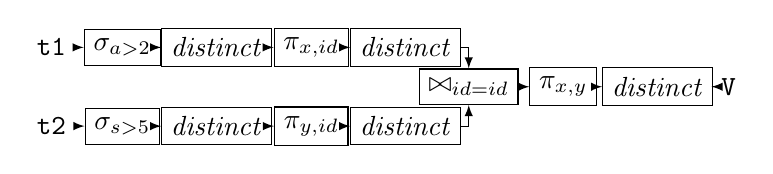
\begin{tikzpicture}[node distance=1.2cm,>=latex]
    \node[] (t1) {\code{t1}};
    \node[block, right of=t1, node distance=.9cm] (s1) {$\sigma_{a > 2}$};
    \node[block, right of=s1] (d1) {$\distinct$};
    \node[block, right of=d1] (p1) {$\pi_{x, id}$};
    \node[block, right of=p1] (d11) {$\distinct$};
    \node[below of=t1, node distance=1cm] (t2) {\code{t2}};
    \node[block, right of=t2, node distance=.9cm] (s2) {$\sigma_{s > 5}$};
    \node[block, right of=s2] (d2) {$\distinct$};
    \node[block, right of=d2] (p2) {$\pi_{y, id}$};
    \node[block, right of=p2] (d21) {$\distinct$};
    \node[below of=d11, node distance=.5cm] (mid) {};
    \node[block, right of=mid, node distance=.8cm] (j) {$\bowtie_{id = id}$};
    \node[block, right of=j] (p) {$\pi_{x, y}$};
    \node[block, right of=p] (d) {$\distinct$};
    \node[right of=d, node distance=.9cm] (V) {\code{V}};
    \draw[->] (t1) -- (s1);
    \draw[->] (s1) -- (d1);
    \draw[->] (d1) -- (p1);
    \draw[->] (p1) -- (d11);
    \draw[->] (t2) -- (s2);
    \draw[->] (s2) -- (d2);
    \draw[->] (d2) -- (p2);
    \draw[->] (p2) -- (d21);
    \draw[->] (d11) -| (j);
    \draw[->] (d21) -| (j);
    \draw[->] (j) -- (p);
    \draw[->] (p) -- (d);
    \draw[->] (d) -- (V);
\end{tikzpicture}

Step 2: apply the rules to eliminate $\distinct$ operators.
First from Proposition~\ref{prop-distinct-once}:

\noindent
\begin{tikzpicture}[node distance=1.2cm,>=latex]
    \node[] (t1) {\code{t1}};
    \node[block, right of=t1, node distance=.9cm] (s1) {$\sigma_{a > 2}$};
    \node[block, right of=s1] (p1) {$\pi_{x, id}$};
    \node[block, right of=p1] (d11) {$\distinct$};
    \node[below of=t1, node distance=1cm] (t2) {\code{t2}};
    \node[block, right of=t2, node distance=.9cm] (s2) {$\sigma_{s > 5}$};
    \node[block, right of=s2] (p2) {$\pi_{y, id}$};
    \node[block, right of=p2] (d21) {$\distinct$};
    \node[below of=d11, node distance=.5cm] (mid) {};
    \node[block, right of=mid, node distance=.8cm] (j) {$\bowtie_{id = id}$};
    \node[block, right of=j] (p) {$\pi_{x, y}$};
    \node[block, right of=p] (d) {$\distinct$};
    \node[right of=d, node distance=.9cm] (V) {\code{V}};
    \draw[->] (t1) -- (s1);
    \draw[->] (s1) -- (p1);
    \draw[->] (p1) -- (d11);
    \draw[->] (t2) -- (s2);
    \draw[->] (s2) -- (p2);
    \draw[->] (p2) -- (d21);
    \draw[->] (d11) -| (j);
    \draw[->] (d21) -| (j);
    \draw[->] (j) -- (p);
    \draw[->] (p) -- (d);
    \draw[->] (d) -- (V);
\end{tikzpicture}

\noindent The rule from Proposition~\ref{prop-distinct-delay} gives
(from now on we omit the subscripts to save space):

\noindent
\begin{tikzpicture}[node distance=1.2cm,>=latex]
    \node[] (t1) {\code{t1}};
    \node[block, right of=t1, node distance=.9cm] (s1) {$\sigma$};
    \node[block, right of=s1] (p1) {$\pi$};
    \node[below of=t1, node distance=1cm] (t2) {\code{t2}};
    \node[block, right of=t2, node distance=.9cm] (s2) {$\sigma$};
    \node[block, right of=s2] (p2) {$\pi$};
    \node[below of=p1, node distance=.5cm] (mid) {};
    \node[block, right of=mid, node distance=.8cm] (j) {$\bowtie$};
    \node[block, right of=j] (d0) {$\distinct$};
    \node[block, right of=d0] (p) {$\pi$};
    \node[block, right of=p] (d) {$\distinct$};
    \node[right of=d, node distance=.9cm] (V) {\code{V}};
    \draw[->] (t1) -- (s1);
    \draw[->] (s1) -- (p1);
    \draw[->] (t2) -- (s2);
    \draw[->] (s2) -- (p2);
    \draw[->] (p1) -| (j);
    \draw[->] (p2) -| (j);
    \draw[->] (j) -- (d0);
    \draw[->] (d0) -- (p);
    \draw[->] (p) -- (d);
    \draw[->] (d) -- (V);
\end{tikzpicture}

\noindent And again~\ref{prop-distinct-once}:

\noindent
\begin{tikzpicture}[node distance=1cm,>=latex]
    \node[] (t1) {\code{t1}};
    \node[block, right of=t1, node distance=.9cm] (s1) {$\sigma$};
    \node[block, right of=s1] (p1) {$\pi$};
    \node[below of=t1, node distance=1cm] (t2) {\code{t2}};
    \node[block, right of=t2, node distance=.9cm] (s2) {$\sigma$};
    \node[block, right of=s2] (p2) {$\pi$};
    \node[below of=p1, node distance=.5cm] (mid) {};
    \node[block, right of=mid, node distance=.8cm] (j) {$\bowtie$};
    \node[block, right of=j] (p) {$\pi$};
    \node[block, right of=p] (d) {$\distinct$};
    \node[right of=d, node distance=1cm] (V) {\code{V}};
    \draw[->] (t1) -- (s1);
    \draw[->] (s1) -- (p1);
    \draw[->] (t2) -- (s2);
    \draw[->] (s2) -- (p2);
    \draw[->] (p1) -| (j);
    \draw[->] (p2) -| (j);
    \draw[->] (j) -- (p);
    \draw[->] (p) -- (d);
    \draw[->] (d) -- (V);
\end{tikzpicture}

At this point no more $\distinct$ elimination rules can be applied.

Step 3: we lift the circuit using distributivity of composition over
lifting (Proposition~\ref{prop:distributivity}); we obtain a circuit
that computes over streams, i.e., for each new input pair of relations
\code{t1} and \code{t2} it will produce an output view \code{V}:

\noindent
\begin{tikzpicture}[node distance=1cm,>=latex]
    \node[] (t1) {\code{t1}};
    \node[block, right of=t1, node distance=.9cm] (s1) {$\lift{\sigma}$};
    \node[block, right of=s1] (p1) {$\lift{\pi}$};
    \node[below of=t1, node distance=1cm] (t2) {\code{t2}};
    \node[block, right of=t2, node distance=.9cm] (s2) {$\lift{\sigma}$};
    \node[block, right of=s2] (p2) {$\lift{\pi}$};
    \node[below of=p1, node distance=.5cm] (mid) {};
    \node[block, right of=mid, node distance=.8cm] (j) {$\lift{\bowtie}$};
    \node[block, right of=j] (p) {$\lift{\pi}$};
    \node[block, right of=p, node distance=1.2cm] (d) {$\lift{\distinct}$};
    \node[right of=d] (V) {\code{V}};
    \draw[->] (t1) -- (s1);
    \draw[->] (s1) -- (p1);
    \draw[->] (t2) -- (s2);
    \draw[->] (s2) -- (p2);
    \draw[->] (p1) -| (j);
    \draw[->] (p2) -| (j);
    \draw[->] (j) -- (p);
    \draw[->] (p) -- (d);
    \draw[->] (d) -- (V);
\end{tikzpicture}

Step 4: incrementalize circuit, obtaining a circuit that computes over changes;
this circuit receives changes to relations \code{t1} and \code{t2} and for each
such change it produces the corresponding change in the output view \code{V}:

\noindent
\begin{tikzpicture}[node distance=1cm,>=latex]
    \node[] (t1) {$\Delta$\code{t1}};
    \node[block, right of=t1, node distance=.8cm] (I1) {$\I$};
    \node[block, right of=I1, node distance=.9cm] (s1) {$\lift{\sigma}$};
    \node[block, right of=s1] (p1) {$\lift{\pi}$};
    \node[below of=t1, node distance=1cm] (t2) {$\Delta$\code{t2}};
    \node[block, right of=t2, node distance=.8cm] (I2) {$\I$};
    \node[block, right of=I2, node distance=.9cm] (s2) {$\lift{\sigma}$};
    \node[block, right of=s2] (p2) {$\lift{\pi}$};
    \node[below of=p1, node distance=.5cm] (mid) {};
    \node[block, right of=mid, node distance=.7cm] (j) {$\lift{\bowtie}$};
    \node[block, right of=j] (p) {$\lift{\pi}$};
    \node[block, right of=p, node distance=1.2cm] (d) {$\lift{\distinct}$};
    \node[block, right of=d, node distance=1.1cm] (D) {$\D$};
    \node[right of=D, node distance=.8cm] (V) {$\Delta$\code{V}};
    \draw[->] (t1) -- (I1);
    \draw[->] (I1) -- (s1);
    \draw[->] (s1) -- (p1);
    \draw[->] (t2) -- (I2);
    \draw[->] (I2) -- (s2);
    \draw[->] (s2) -- (p2);
    \draw[->] (p1) -| (j);
    \draw[->] (p2) -| (j);
    \draw[->] (j) -- (p);
    \draw[->] (p) -- (d);
    \draw[->] (d) -- (D);
    \draw[->] (D) -- (V);
\end{tikzpicture}

Step 5: apply the chain rule to rewrite the circuit as a composition of incremental operators;

\noindent
\begin{tikzpicture}[node distance=1.6cm,>=latex]
    \node[] (t1) {$\Delta$\code{t1}};
    \node[block, right of=t1, node distance=1.2cm] (s1) {$\inc{(\lift{\sigma})}$};
    \node[block, right of=s1] (p1) {$\inc{(\lift{\pi})}$};
    \node[below of=t1, node distance=1.2cm] (t2) {$\Delta$\code{t2}};
    \node[block, right of=t2, node distance=1.2cm] (s2) {$\inc{(\lift{\sigma})}$};
    \node[block, right of=s2] (p2) {$\inc{(\lift{\pi})}$};
    \node[below of=p1, node distance=.6cm] (mid) {};
    \node[block, right of=mid, node distance=.8cm] (j) {$\inc{(\lift{\bowtie})}$};
    \node[block, right of=j] (p) {$\inc{(\lift{\pi})}$};
    \node[block, right of=p] (d) {$\inc{(\lift{\distinct})}$};
    \node[right of=d, node distance=1.2cm] (V) {$\Delta$\code{V}};.8
    \draw[->] (t1) -- (s1);
    \draw[->] (s1) -- (p1);
    \draw[->] (t2) -- (s2);
    \draw[->] (s2) -- (p2);
    \draw[->] (p1) -| (j);
    \draw[->] (p2) -| (j);
    \draw[->] (j) -- (p);
    \draw[->] (p) -- (d);
    \draw[->] (d) -- (V);
\end{tikzpicture}

Use the linearity of $\sigma$ and $\pi$ to simplify this circuit (notice that
all linear operators no longer have a $\inc{\cdot}$):

\noindent
\begin{tikzpicture}[node distance=1cm,>=latex]
    \node[] (t1) {$\Delta$\code{t1}};
    \node[block, right of=t1, node distance=1cm] (s1) {$\lift{\sigma}$};
    \node[block, right of=s1] (p1) {$\lift{\pi}$};
    \node[below of=t1, node distance=1.2cm] (t2) {$\Delta$\code{t2}};
    \node[block, right of=t2, node distance=1cm] (s2) {$\lift{\sigma}$};
    \node[block, right of=s2] (p2) {$\lift{\pi}$};
    \node[below of=p1, node distance=.6cm] (mid) {};
    \node[block, right of=mid, node distance=.8cm] (j) {$\inc{(\lift{\bowtie})}$};
    \node[block, right of=j] (p) {$\lift{\pi}$};
    \node[block, right of=p, node distance=1.2cm] (d) {$\inc{(\lift{\distinct})}$};
    \node[right of=d, node distance=1.3cm] (V) {$\Delta$\code{V}};
    \draw[->] (t1) -- (s1);
    \draw[->] (s1) -- (p1);
    \draw[->] (t2) -- (s2);
    \draw[->] (s2) -- (p2);
    \draw[->] (p1) -| (j);
    \draw[->] (p2) -| (j);
    \draw[->] (j) -- (p);
    \draw[->] (p) -- (d);
    \draw[->] (d) -- (V);
\end{tikzpicture}

Finally, replace the incremental join using the formula for bilinear operators
(Theorem~\ref{bilinear}),
and the incremental $\distinct$ (Proposition~\ref{prop-inc_distinct}),
obtaining the following circuit:

\noindent
\begin{tikzpicture}[node distance=.8cm,>=latex]
    \node[] (t1) {$\Delta$\code{t1}};
    \node[block, right of=t1] (s1) {$\lift{\sigma}$};
    \node[block, right of=s1] (p1) {$\lift{\pi}$};
    \node[below of=t1, node distance=.8cm] (t2) {$\Delta$\code{t2}};
    \node[block, right of=t2] (s2) {$\lift{\sigma}$};
    \node[block, right of=s2] (p2) {$\lift{\pi}$};

    % join expansion
      \node[block, right of=p1] (jI1) {$\I$};
      \node[block, right of=p2] (jI2) {$\I$};
      \draw[->] (p1) -- (jI1);
      \draw[->] (p2) -- (jI2);
      \node[block, right of=jI2] (ZI2) {$\zm$};
      \draw[->] (jI2) -- (ZI2);
      \node[block, right of=jI1] (DI1) {$\lift\bowtie$};
      \node[block, right of=ZI2, node distance=1cm] (DI2) {$\lift\bowtie$};
      \draw[->] (jI1) -- (DI1);
      \draw[->] (ZI2) -- (DI2);
      \node[block, circle, above of=DI2, inner sep=0cm] (sum) {$+$};
      \draw[->] (DI1) -- (sum);
      \draw[->] (DI2) -- (sum);
      \draw[->] (p1) -- (DI2);
      \draw[->] (p2) -- (DI1);

    \node[block, right of=sum] (p) {$\lift{\pi}$};
    \draw[->] (sum) -- (p);
    \node[block, right of=p] (Id) {$\I$};
    \node[block, right of=Id] (zd) {$\zm$};
    \node[block, below of=zd] (H) {$\lift{H}$};
    \node[right of=H] (V) {$\Delta$\code{V}};
    \draw[->] (t1) -- (s1);
    \draw[->] (s1) -- (p1);
    \draw[->] (t2) -- (s2);
    \draw[->] (s2) -- (p2);
    \draw[->] (p) -- node (tapp) {} (Id);
    \draw[->] (Id) -- (zd);
    \draw[->] (zd) -- (H);
    \draw[->] (tapp.center) |- (H);
    \draw[->] (H) -- (V);
\end{tikzpicture}

Notice that the resulting circuit contains three integration
operations: two from the join, and one from the $\distinct$.  It also
contains two join operators.  However, the work performed by each
operator for each new input is proportional to the size of the change.


\section{Incremental computation}\label{sec:incremental}

In this section we formally define incremental computations over
streams and analyze their properties.

\begin{definition}\label{def:inc}
Given a unary stream operator $Q: \stream{A} \to \stream{B}$ we define the
\defined{incremental version} of $Q$ as $\inc{Q} \defn \D \circ Q \circ \I$.
$\inc{Q}$ has the same ``type'' as $Q$: $\inc{Q}: \stream{A} \to \stream{B}$.
For an operator with multiple inputs we define
the incremental version by applying $\I$ to each input independently:
e.g., if $T: \stream{A} \times \stream{B} \rightarrow \stream{C}$ then
$\inc{T}: \stream{A} \times \stream{B} \rightarrow \stream{C}$
and $\inc{T}(a, b) \defn \D (T(\I(a), \I(b)))$.
\end{definition}

The following diagram illustrates the intuition behind this definition:

\begin{center}
\begin{tikzpicture}[auto,>=latex]
    \node[] (input) {$\Delta s$};
    \node[block, right of=input] (I) {$\I$};
    \node[block, right of=I] (Q) {$Q$};
    \node[block, right of=Q] (D) {$\D$};
    \node[right of=D] (output) {$\Delta o$};
    \draw[->] (input) -- (I);
    \draw[->] (I) -- node (s) {$s$} (Q);
    \draw[->] (Q) -- node (o) {$o$} (D);
    \draw[->] (D) -- (output);
\end{tikzpicture}
\end{center}

If $Q(s) = o$ is a computation, then $\inc{Q}$ performs
the ``same'' computation as $Q$,
but between streams of changes $\Delta s$ and $\Delta o$.
This is the diagram from the
introduction, substituting $\Delta s$ for the transaction stream $T$,
and $o$ for the stream of view versions $V$.

Notice that our definition of incremental computation is meaningful only for \emph{streaming}
computations; this is in contrast to classic definitions, e.g.~\cite{gupta-idb95} which
consider only one change.  Generalizing the definition to operate on streams gives us
additional power, especially when operating with recursive queries.

The following proposition is one of our central results.

\begin{proposition}(Properties of the incremental version):\\
\label{prop-inc-properties}
For computations of appropriate types, the following hold:
\begin{description}
\item[inversion:] $Q\mapsto\inc{Q}$ is bijective; its inverse is $Q\mapsto \I\circ Q\circ\D$.
\item[invariance:] $\inc{+} = +, \inc{(\zm)} = \zm, \inc{-} = -, \inc{\I}=\I, \inc{\D}=\D$
\item[push/pull:]
    $Q \circ \I = \I \circ \inc{Q}$; $\D\circ Q = \inc{Q}\circ\D$
\item[chain:] $\inc{(Q_1\circ Q_2)} = \inc{Q_1}\circ\inc{Q_2}$ (This generalizes to operators with multiple inputs.)
\item[add:] $\inc{(Q_1 + Q_2)} = \inc{Q_1} + \inc{Q_2}$
\item[cycle:] $\inc{(\lambda s. \fix{\alpha}{T(s,\zm(\alpha)}))} = \lambda s. \fix{\alpha}{\inc{T}(s,\zm(\alpha)})$
\end{description}
\end{proposition}
\begin{proof}

The inversion and push-pull properties follow straightforwardly from the fact
that $\I$ and $\D$ are inverses of each other.

For proving invariance we have $\inc{+}(a, b) \defn \D(\I(a) + \I(b)) = a + b$, due to
linearity of $\I$.
$\inc{-}(a) = \D(-\I(a)) = \D(0 - \I(a)) = \D(\I(0) - \I(a)) = \D(\I(0 - a)) = -a$,
also due to linearity of $\I$.

The chain rule follows from push-pull. Indeed,
$$
\I\circ\inc{Q_1}\circ\inc{Q_2}=Q_1\circ\I\circ\inc{Q_2}=Q_1\circ Q_2\circ\I
$$

I.e., we have the following sequence of equivalent circuits:

\begin{center}
\begin{tabular}{m{7.5cm}m{1cm}}
\begin{tikzpicture}[auto,>=latex]
  \node[] (input) {$i$};
  \node[block, right of=input] (I) {$\I$};
  \node[block, right of=I] (Q1) {$Q_1$};
  \node[block, right of=Q1] (Q2) {$Q_2$};
  \node[block, right of=Q2] (D) {$\D$};
  \node[right of=D] (output)  {$o$};
  \draw[->] (input) -- (I);
  \draw[->] (I) -- (Q1);
  \draw[->] (Q1) -- (Q2);
  \draw[->] (Q2) -- (D);
  \draw[->] (D) -- (output);
\end{tikzpicture}
& $\cong$ \\
\begin{tikzpicture}[auto,>=latex]
  \node[] (input) {$i$};
  \node[block, right of=input] (I) {$\I$};
  \node[block, right of=I] (Q1) {$Q_1$};
  \node[block, right of=Q1] (D1) {$\D$};
  \node[block, right of=D1] (I1) {$\I$};
  \node[block, right of=I1] (Q2) {$Q_2$};
  \node[block, right of=Q2] (D) {$\D$};
  \node[right of=D] (output)  {$o$};
  \draw[->] (input) -- (I);
  \draw[->] (I) -- (Q1);
  \draw[->] (Q1) -- (D1);
  \draw[->] (D1) -- (I1);
  \draw[->] (I1) -- (Q2);
  \draw[->] (Q2) -- (D);
  \draw[->] (D) -- (output);
\end{tikzpicture} & $\cong$ \\
%\noindent which, due to associativity of function composition, is the same as:
\begin{tikzpicture}[auto,>=latex]
  \node[] (input) {$i$};
  \node[block, right of=input] (Q1) {$\inc{Q_1}$};
  \node[block, right of=Q1, node distance=1.5cm] (Q2) {$\inc{Q_2}$};
  \node[right of=Q2] (output)  {$o$};
  \draw[->] (input) -- (Q1);
  \draw[->] (Q1) -- (Q2);
  \draw[->] (Q2) -- (output);
\end{tikzpicture}
\end{tabular}
\end{center}

Here is a version of the chain rule with a binary operator:

\begin{center}
\begin{tabular}{m{7.5cm}m{1cm}}
\begin{tikzpicture}[auto,node distance=1cm,>=latex]
    \node[] (a) {$a$};
    \node[block, right of=a] (ai) {$\I$};
    \node[below of=a] (b) {$b$};
    \node[block, right of=b] (bi) {$\I$};
    \node[block, right of=ai] (q1) {$Q_1$};
    \node[below of=q1, node distance=.5cm] (midway) {};
    \node[block, right of=bi] (q2) {$Q_2$};
    \node[block, right of=midway] (q) {$T$};
    \node[block, right of=q] (D) {$\D$};
    \node[right of=D] (output) {$o$};
    \draw[->] (a) -- (ai);
    \draw[->] (b) -- (bi);
    \draw[->] (ai) -- (q1);
    \draw[->] (bi) -- (q2);
    \draw[->] (q1) -| (q);
    \draw[->] (q2) -| (q);
    \draw[->] (q) -- (D);
    \draw[->] (D) -- (output);
\end{tikzpicture}
& $\cong$ \\
\begin{tikzpicture}[auto,node distance=1cm,>=latex]
    \node[] (a) {$a$};
    \node[block, right of=a] (ai) {$\I$};
    \node[block, right of=ai] (q1) {$Q_1$};
    \node[block, right of=q1] (d1) {$\D$};
    \node[block, right of=d1] (i1) {$\I$};

    \node[below of=a] (b) {$b$};
    \node[block, right of=b] (bi) {$\I$};
    \node[block, right of=bi] (q2) {$Q_2$};
    \node[block, right of=q2] (d2) {$\D$};
    \node[block, right of=d2] (i2) {$\I$};

    \node[below of=i1, node distance=.5cm] (midway) {};
    \node[block, right of=midway] (q) {$T$};
    \node[block, right of=q] (D) {$\D$};
    \node[right of=D] (output) {$o$};
    \draw[->] (a) -- (ai);
    \draw[->] (ai) -- (q1);
    \draw[->] (q1) -- (d1);
    \draw[->] (d1) -- (i1);

    \draw[->] (b) -- (bi);
    \draw[->] (bi) -- (q2);
    \draw[->] (q2) -- (d2);
    \draw[->] (d2) -- (i2);

    \draw[->] (i1) -| (q);
    \draw[->] (i2) -| (q);
    \draw[->] (q) -- (D);
    \draw[->] (D) -- (output);
\end{tikzpicture} & $\cong$ \\
\begin{tikzpicture}[auto,node distance=1cm,>=latex]
    \node[] (a) {$a$};
    \node[below of=a] (b) {$b$};
    \node[block, right of=a] (q1) {$\inc{Q_1}$};
    \node[below of=q1, node distance=.5cm] (midway) {};
    \node[block, right of=b] (q2) {$\inc{Q_2}$};
    \node[block, right of=midway] (q) {$\inc{T}$};
    \node[right of=q] (output) {$o$};
    \draw[->] (a) -- (q1);
    \draw[->] (b) -- (q2);
    \draw[->] (q1) -| (q);
    \draw[->] (q2) -| (q);
    \draw[->] (q) -- (output);
\end{tikzpicture}
\end{tabular}
\end{center}

The add rule follows from push/pull and the linearity of $\I$ (or $\D$). Indeed,
$$
\I\circ(\inc{Q_1}+\inc{Q_2})=\I\circ\inc{Q_1}+\I\circ\inc{Q_2}=
Q_1\circ\I+ Q_2\circ\I = (Q_1+Q_2)\circ\I
$$

I.e., the following diagrams are equivalent:

\begin{center}
\begin{tabular}{m{6cm}m{1cm}}
\begin{tikzpicture}[auto,>=latex]
  \node[] (input) {$i$};
  \node[block, right of=input] (I) {$\I$};
  \node[block, above right=0cm and 1cm of I] (Q1) {$Q_1$};
  \node[block, below right=0cm and 1cm of I] (Q2) {$Q_2$};
  \node[block, shape=circle, right of=I, node distance=2.5cm, inner sep=0pt] (plus) {$+$};
  \node[block, right of=plus,node distance=1cm] (D) {$\D$};
  \node[right of=D] (output) {$o$};
  \draw[->] (input) -- (I);
  \draw[<-] (Q1.west) -- ++(-5mm,0) |- (I);
  \draw[<-] (Q2.west) -- ++(-5mm,0) |- (I);
  \draw[->] (Q1) -| (plus);
  \draw[->] (Q2) -| (plus);
  \draw[->] (plus) -- (D);
  \draw[->] (D) -- (output);
\end{tikzpicture}
& $\cong$ \\
\begin{tikzpicture}[auto,>=latex]
  \node[] (input) {$i$};
  \node[block, above right=0cm and 1cm of input] (I1) {$\I$};
  \node[block, below right=0cm and 1cm of input] (I2) {$\I$};
  \node[block, right of=I1] (Q1) {$Q_1$};
  \node[block, right of=I2] (Q2) {$Q_2$};
  \node[block, right of=Q1] (D1) {$\D$};
  \node[block, right of=Q2] (D2) {$\D$};
  \node[block, shape=circle, right of=input, node distance=4cm, inner sep=0pt] (plus) {$+$};
  \node[right of=plus] (output) {$o$};
  \draw[<-] (I1.west) -- ++(-5mm,0) |- (input);
  \draw[<-] (I2.west) -- ++(-5mm,0) |- (input);
  \draw[->] (I1) -- (Q1);
  \draw[->] (I2) -- (Q2);
  \draw[->] (Q1) -- (D1);
  \draw[->] (Q2) -- (D2);
  \draw[->] (D1) -| (plus);
  \draw[->] (D2) -| (plus);
  \draw[->] (plus) -- (output);
\end{tikzpicture} & $\cong$ \\
\begin{tikzpicture}[auto,>=latex]
  \node[] (input) {$i$};
  \node[block, above right=0cm and 1cm of input] (Q1) {$\inc{Q_1}$};
  \node[block, below right=0cm and 1cm of input] (Q2) {$\inc{Q_2}$};
  \node[block, shape=circle, right of=input, node distance=2.5cm, inner sep=0pt] (plus) {$+$};
  \node[right of=plus] (output) {$o$};
  \draw[<-] (Q1.west) -- ++(-5mm,0) |- (input);
  \draw[<-] (Q2.west) -- ++(-5mm,0) |- (input);
  \draw[->] (Q1) -| (plus);
  \draw[->] (Q2) -| (plus);
  \draw[->] (plus) -- (output);
\end{tikzpicture}
\end{tabular}
\end{center}

The cycle rule is most interesting. First, observe that if $T$ is causal then so is
$\inc{T}$ thus both sides of the
equality are well-defined. Next, we can use again push/pull to show the equality
if we can check that
$$
\I\circ(\lambda s. \fix{\alpha}{\inc{T}(s,\zm(\alpha)}) =
(\lambda s. \fix{\alpha}{T(s,\zm(\alpha)})\circ\I
$$
that is, for any $s$,
$$
\I(\fix{\alpha}{\inc{T}(s,\zm(\alpha)}) =
\fix{\alpha}{T(\I(s),\zm(\alpha)})
$$
This follows from the following lemma.
\end{proof}

\begin{lemma}
\label{lemma-delta-fix}
If the parameters $a$ and $b$ are related by $b=\D(a)$ (equivalently $a=\I(b)$)
then the unique solutions of the fixed point equations
$$
\alpha~=~ T(a,\zm(\alpha))~~~~\mbox{and}~~~~
\beta~=~\inc{T}(b,\zm(\beta))
$$
are related by $\alpha=\I(\beta)$ (equivalently $\beta=\D(\alpha)$).
\end{lemma}
\begin{proof} (Of Lemma~\ref{lemma-delta-fix})
Let $\beta$ be the unique solution of $\beta~=~\inc{T}(\D(a),\zm(\beta))$. We verify that
$\alpha=\I(\beta)$ satisfies the equation $\alpha~=~ T(a,\zm(\alpha))$. Indeed, using the fact that $\I$ and $\D$ are inverses as well as the time-invariance of $\I$ we have
\begin{eqnarray*}
\I(\beta) & = & \I(\inc{T}(\D(a),\zm(\beta)))\\
          & = & \I(\D(T(\I(\D(a)),\I(\zm(\beta))))\\
          & = & T(a,\I(\zm(\beta))\\
          & = & T(a,\zm(\I(\beta))
\end{eqnarray*}

I.e., starting from this diagram we apply a sequence of term-rewriting se\-man\-tics-preserving
transformations:

\begin{center}
\begin{tabular}{m{5.5cm}m{1cm}}
\begin{tikzpicture}[>=latex]
    \node[] (input) {$s$};
    \node[block, right of=input] (I) {$\I$};
    \node[block, right of=I] (f) {$T$};
    \node[block, right of=f, node distance=1.5cm] (D) {$\D$};
    \node[right of=D] (output) {$o$};
    \node[block, below of=f] (z) {$\zm$};
    \draw[->] (input) -- (I);
    \draw[->] (I) -- (f);
    \draw[->] (f) -- node (mid) {} (D);
    \draw[->] (mid.center) |-  (z);
    \draw[->] (z.west) -- ++(-.3,0) |- ([yshift=1mm]f.south west);
    \draw[->] (D) -- (output);
\end{tikzpicture} & $\cong$ \\
\begin{tikzpicture}[>=latex]
    \node[] (input) {$s$};
    \node[block, right of=input] (I) {$\I$};
    \node[block, below of=I] (D0) {$\D$};
    \node[block, right of=D0] (I0) {$\I$};
    \node[above of=I0, node distance=.5cm] (midway) {};

    \node[block, right of=midway] (f) {$T$};
    \node[block, right of=f] (D) {$\D$};
    \node[right of=D] (output) {$o$};
    \node[block, below of=f, node distance=1.5cm] (I1) {$\I$};
    \node[block, left of=I1] (z) {$\zm$};
    \draw[->] (input) -- (I);
    \draw[->] (I) -| (f);
    \draw[->] (D0) -- (I0);
    \draw[->] (I0) -| (f);
    \draw[->] (f) -- (D);
    \draw[->] (D) -- node (mid) {} (output);
    \draw[->] (mid.center) |-  (I1);
    \draw[->] (I1) -- (z);
    \draw[->] (z.west) -- ++(-1.5,0) |- (D0);
\end{tikzpicture} & $\cong$ \\
\begin{tikzpicture}[>=latex]
    \node[] (input) {$s$};
    \node[block, right of=input] (f) {$\inc{T}$};
    \node[right of=f, node distance=1.5cm] (output) {$o$};
    \node[block, below of=f] (z) {$\zm$};
    \draw[->] (input) -- (f);
    \draw[->] (f) -- node (mid) {} (output);
    \draw[->] (mid.center) |-  (z);
    \draw[->] (z.west) -- ++(-.3,0) |- ([yshift=1mm]f.south west);
\end{tikzpicture}
\end{tabular}
\end{center}

\end{proof}

If we specialize the above formula for the case $T(a,b) = Q(a+b)$
(for some time-invariant operator $Q$), by us the linearity of $\I$
we get that:

\noindent
\begin{tabular}{m{6cm}m{0.5cm}m{4cm}}
\begin{tikzpicture}[auto,>=latex]
  \node[] (input) {$i$};
  \node[block, right of=input] (I0) {$\I$};
  \node[block, shape=circle, right of=I0, inner sep=0in] (plus) {$+$};
  \node[block, right of=plus] (q) {$Q$};
  \node[block, right of=q, node distance=1.5cm] (D) {$\D$};
  \node[right of=D] (output)  {$o$};
  \draw[->] (input) -- (I0);
  \draw[->] (I0) -- (plus);
  \draw[->] (plus) -- (q);
  \draw[->] (q) -- node (o) {} (D);
  \draw[->] (D) -- (output);
  \node[block, below of=q] (z) {$\zm$};
  \draw[->] (o) |- (z);
  \draw[->] (z) -| (plus);
\end{tikzpicture} & $\cong$ &
\begin{tikzpicture}[auto,>=latex]
  \node[] (input) {$i$};
  \node[block, shape=circle, right of=input, inner sep=0in] (plus) {$+$};
  \node[block, right of=plus] (q) {$\inc{Q}$};
  \node[right of=q, node distance=1.5cm] (output)  {$o$};
  \draw[->] (input) -- (plus);
  \draw[->] (plus) -- (q);
  \draw[->] (q) -- node (o) {} (output);
  \node[block, below of=q] (z) {$\zm$};
  \draw[->] (o) |- (z);
  \draw[->] (z) -| (plus);
\end{tikzpicture}
\end{tabular}

\begin{comment}
& \mbox{Initial form} \\
\begin{tikzpicture}[auto,>=latex]
  \node[] (input) {$i$};
  \node[block, right of=input] (D0) {$\D$};
  \node[block, right of=D0] (I0) {$\I$};
  \node[block, shape=circle, right of=I0, inner sep=0in] (plus) {$+$};
  \node[block, right of=plus] (q) {$Q$};
  \node[right of=q, node distance=4cm] (output)  {$o$};
  \draw[->] (input) -- (D0);
  \draw[->] (D0) -- (I0);
  \draw[->] (I0) -- (plus);
  \draw[->] (plus) -- (q);
  \draw[->] (q) -- node [pos=0.8] (o) {} (output);
  \node[block, below of=q] (I1) {$\I$};
  \node[block, right of=I1] (D1) {$\D$};
  \node[block, right of=D1] (z) {$\zm$};
  \draw[->] (o) |- (z);
  \draw[->] (z) -- (D1);
  \draw[->] (D1) -- (I1);
  \draw[->] (I1) -| (plus);
\end{tikzpicture} & \I \circ \D = \id \\
\begin{tikzpicture}[auto,>=latex]
  \node[] (input) {$i$};
  \node[block, right of=input] (D0) {$\D$};
  \node[block, shape=circle, right of=D0, inner sep=0in] (plus) {$+$};
  \node[block, right of=plus] (I) {$\I$};
  \node[block, right of=I] (q) {$Q$};
  \node[right of=q, node distance=2cm] (output)  {$o$};
  \draw[->] (input) -- (D0);
  \draw[->] (D0) -- (plus);
  \draw[->] (plus) -- (I);
  \draw[->] (I) -- (q);
  \draw[->] (q) -- node (o) {} (output);
  \node[block, below of=I] (z) {$\zm$};
  \node[block, right of=z] (D1) {$\D$};
  \draw[->] (o) |- (D1);
  \draw[->] (D1) -- (z);
  \draw[->] (z) -| (plus);but not
\end{tikzpicture} & \mbox{Linearity of }\I  \\
\begin{tikzpicture}[auto,>=latex]
  \node[] (input) {$i$};
  \node[block, right of=input] (D0) {$\D$};
  \node[block, shape=circle, right of=D0, inner sep=0in] (plus) {$+$};
  \node[block, right of=plus] (I) {$\I$};
  \node[block, right of=I] (q) {$Q$};
  \node[block, right of=q] (D1) {$\D$};
  \node[block, right of=D1] (I2) {$\I$};
  \node[right of=I2, node distance=2cm] (output)  {$o$};
  \draw[->] (input) -- (D0);
  \draw[->] (D0) -- (plus);
  \draw[->] (plus) -- (I);
  \draw[->] (I) -- (q);
  \draw[->] (q) -- (D1);
  \draw[->] (D1) -- (I2);
  \draw[->] (I2) -- node (o) {} (output);
  \node[block, below of=I] (z) {$\zm$};
  \node[block, right of=z] (D1) {$\D$};
  \draw[->] (o) |- (D1);
  \draw[->] (D1) -- (z);
  \draw[->] (z) -| (plus);
\end{tikzpicture} & \D \circ \I = \id \\
\end{comment}


%\subsection{Linear operators}

\begin{theorem}[Linear]\label{linear}
For any LTI operator $Q$ we have $\inc{Q}=Q$.
\end{theorem}

\begin{proof}
By the push/pull rule from Proposition~\ref{prop-inc-properties}
it suffices to show that $Q$ commutes with differentiation:
$$
\begin{aligned}
  \D(Q(s)) &= Q(s)-\zm(Q(s)) & \mbox{by definition of }\D \\
  &= Q(s)-Q(\zm(s)) & \mbox{by time-invariance of }Q \\
  &= Q(s-\zm(s)) & \mbox{by linearity of }Q \\
  &= Q(\D(s)) & \mbox{by definition of }\D.
\end{aligned}
$$
\end{proof}


As we have shown, the incremental version of a linear unary operator equals the operator itself.
However, this is not true, in general, for multilinear operators. Nonetheless, there is a useful relationship
between the incremental version of a multilinear operator and the operator itself. We illustrate with bilinear
operators.
\begin{comment}
\val{Such as join. from incremental maintenance literature recall the definition of "delta" for join:
$\Delta(R\bowtie S) = R\bowtie(\Delta S) \cup (\Delta R)\bowtie S \cup (\Delta R)\bowtie(\Delta S)$.}
\mihai{Indeed, the join is the main application.  Should we hint at this?  It's the first
time the relational algebra will appear in this text.}
\end{comment}

\begin{theorem}[Bilinear]\label{bilinear}
For any bilinear time-invariant operator $\times$ we have
$\inc{(a \times b)} ~=~ a \times b ~+~ \I(\zm(a)) \times b ~+~ a \times \I(\zm(b))$.
\end{theorem}

By rewriting this statement using $\Delta a$ for the stream of changes to $a$ we
get the familiar formula for incremental joins:
$\Delta(a\times b) =\Delta a \times \Delta b + a\times(\Delta b) + (\Delta a)\times b$.

In other words, the following three diagrams are equivalent:

\noindent
\begin{tabular}{m{3.0cm}m{0cm}m{3.5cm}m{0cm}m{3.5cm}}
\begin{tikzpicture}[auto,node distance=.8cm,>=latex]
    \node[] (a) {$a$};
    \node[block, right of=a] (ai) {$\I$};
    \node[below of=a, node distance=.8cm] (midway) {};
    \node[below of=midway, node distance=.8cm] (b) {$b$};
    \node[block, right of=b] (bi) {$\I$};
    \node[block, right of=midway, node distance=1.4cm] (q) {$\times$};
    \node[block, right of=q] (D) {$\D$};
    \node[right of=D] (output) {$o$};
    \draw[->] (a) -- (ai);
    \draw[->] (b) -- (bi);
    \draw[->] (ai) -| (q);
    \draw[->] (bi) -| (q);
    \draw[->] (q) -- (D);
    \draw[->] (D) -- (output);
\end{tikzpicture} &
$\cong$ &
\begin{tikzpicture}[auto,>=latex]
  \node[] (a) {$a$};
  \node[below of=input1, node distance=2cm] (b) {$b$};
  \node[block, right of=a, node distance=.7cm] (I1) {$\I$};
  \node[block, below of=I1] (ab) {$\times$};
  \node[block, right of=b, node distance=.7cm] (I2) {$\I$};
  \draw[->] (a) -- (I1);
  \draw[->] (b) -- (I2);
  \draw[->] (a) |- ([yshift=-1mm]ab.north west);
  \draw[->] (b) |- ([yshift=1mm]ab.south west);
  \node[block, right of=I1] (ZI1) {$\zm$};
  \node[block, right of=I2] (ZI2) {$\zm$};
  \draw[->] (I1) -- (ZI1);
  \draw[->] (I2) -- (ZI2);
  \node[block, right of=ZI1] (DI1) {$\times$};
  \node[block, right of=ZI2] (DI2) {$\times$};
  \draw[->] (ZI1) -- (DI1);
  \draw[->] (ZI2) -- (DI2);
  \node[block, circle, right of=ab, inner sep=0cm, node distance=2cm] (sum) {$+$};
  \draw[->] (ab) -- (sum);
  \draw[->] (DI1) -- (sum);
  \draw[->] (DI2) -- (sum);
  \node[right of=sum, node distance=.7cm] (output) {$o$};
  \draw[->] (sum) -- (output);
  \draw[->] (a) -- (DI2);
  \draw[->] (b) -- (DI1);
\end{tikzpicture} &
$\cong$ &
\begin{tikzpicture}[auto,>=latex]
  \node[] (input1) {$a$};
  \node[below of=input1, node distance=1.5cm] (input2) {$b$};
  \node[block, right of=input1, node distance=.5cm] (I1) {$\I$};
  \node[block, right of=input2, node distance=.5cm] (I2) {$\I$};
  \draw[->] (input1) -- (I1);
  \draw[->] (input2) -- (I2);
  \node[block, right of=I2] (ZI2) {$\zm$};
  \draw[->] (I2) -- (ZI2);
  \node[block, right of=I1] (DI1) {$\times$};
  \node[block, right of=ZI2] (DI2) {$\times$};
  \draw[->] (I1) -- (DI1);
  \draw[->] (ZI2) -- (DI2);
  \node[block, circle, above of=DI2, inner sep=0cm, node distance=.8cm] (sum) {$+$};
  \draw[->] (DI1) -- (sum);
  \draw[->] (DI2) -- (sum);
  \node[right of=sum, node distance=.7cm] (output) {$o$};
  \draw[->] (sum) -- (output);
  \draw[->] (input1) -- (DI2);
  \draw[->] (input2) -- (DI1);
\end{tikzpicture}
\end{tabular}
\begin{proof}
$$
\begin{aligned}
\inc{(a \times b)} &= \D(\I(a) \times \I(b)) & \mbox{def of } \inc{\cdot} \\
             &= (\I(a) \times \I(b)) ~-~  \zm(\I(a) \times \I(b)) & \mbox{def of } \D \\
             &= \I(a) \times \I(b) ~-~  \zm(\I(a)) \times \zm(\I(b)) & \times \mbox{ time inv.}\\
             &= (a + \zm(\I(a))) \times (b + \zm(\I(b))) ~-~ \zm(\I(a)) \times \zm(\I(b)) & \mbox { $\I$ fixpoint equation } \\
             &= a \times b + \zm(\I(a)) \times b + a \times \zm(\I(b)) + \zm(\I(a)) \times \zm(\I(b)) & \\
             &  ~~~~~~~~~~~~~~-~ \zm(\I(a)) \times \zm(\I(b)) & \mbox{bilinearity} \\
             &= a \times b ~+~ \zm(\I(a)) \times b ~+~ a \times \zm(\I(b)) & \mbox{cancel} \\
             &= a \times b ~+~ \I(\zm(a)) \times b ~+~ a \times \I(\zm(b)) & \mbox{$I$ time inv.} \\
             &= (a + \I(\zm(a))) \times b ~+~ a \times \I(\zm(b)) & \mbox{commutativity} \\
             &= \I(a) \times b ~+~ a \times \I(\zm(b)) & \mbox{def of } \I \\
\end{aligned}
$$
\end{proof}

\begin{comment}
\subsection{Vector representations}\label{sec:vector-picture}

Some formulas are easier to read as mathematical expressions over ``vectors''.
We will use the following representation to depict a fragment of a stream $s$:

$\strm{0}{0}$

This ``vector'' representation fixes a time $t$ and shows the integral of the stream prefix
up to $\I(s)[t-1]$ as a rectangle, and $s[t]$ as a square.  We will use a grey rectangle to
show which part of a stream participates in a computation.  For example, we have the following
notations:

$$
\begin{aligned}
\strm{0 0} &= 0 \\
\strm{0 1} &= s[t] \\
\strm{1 0} &= \I(s)[t-1] = \zm(\I(s))[t] \\
\strm{1 1} &= \I(s)[t-1] + s[t] = \I(s)[t]
\end{aligned}
$$

Using this notation, the incremental version of a function $f$ is defined
as $\inc{f}(\strm{0}{1}) = f(\strm{1}{1}) - f(\strm{1}{0})$.

Theorem~\ref{linear} states that for a linear function $f$ we have: \\
$f(\strm{1 1}) - f(\strm{1 0}) = f(\strm{0 1}).$

The statement of Theorem~\ref{bilinear}, for a bilinear stream operation
$\times$ can be written as:
$$
\begin{aligned}
\strm{1 1} \times \strm{1 1} = &
\matmult{\strm{1 0}}{\strm{1 0}} \\ + &
\matmult{\strm{1 0}}{\strm{0 1}} \\ + &
\matmult{\strm{0 1}}{\strm{1 0}} \\ + &
\matmult{\strm{0 1}}{\strm{0 1}}.
\end{aligned}
$$

By definition $\inc{\times}$ is:
$$
\begin{aligned}
\matmult{\strm{1 1}}{\strm{1 1}} - \\
\matmult{\strm{1 0}}{\strm{1 0}} = &
\matmult{\strm{1 0}}{\strm{0 1}} \\ + &
\matmult{\strm{0 1}}{\strm{1 0}} \\ + &
\matmult{\strm{0 1}}{\strm{0 1}}.
\end{aligned}
$$
\end{comment}

\section{Incremental relational queries}\label{sec:inc-relational}

We start by giving a few rules that can be used to optimize relational
\dbsp circuits.  Later we show how \dbsp relational circuits can be
converted to incremental versions.

\subsection{Optimizing $\distinct$}\label{sec:optimizations}

All standard algebraic properties
of the relational operators can be used to optimize circuits.  In addition,
a few optimizations are related to the $\distinct$ operator, which is
not linear, and thus expensive to incrementalize:

\begin{proposition}\label{prop-distinct-delay}
Let Q be one of the following \zrs operators: filtering $\sigma$,
join $\bowtie$, or Cartesian product $\times$.
Then we have $\forall i \in \Z[I], \ispositive(i) \Rightarrow Q(\distinct(i)) = \distinct(Q(i))$.
\end{proposition}

\begin{center}
\begin{tabular}{m{3.5cm}m{.5cm}m{3.5cm}}
\begin{tikzpicture}[auto,>=latex]
  \node[] (input) {$i$};
  \node[block, right of=input, node distance=1.1cm] (distinct) {$\distinct$};
  \node[block, right of=distinct, node distance=1.2cm] (q) {$Q$};
  \node[right of=q] (output)  {$o$};
  \draw[->] (input) -- (distinct);
  \draw[->] (distinct) -- (q);
  \draw[->] (q) -- (output);
\end{tikzpicture}
&
$\cong$
&
\begin{tikzpicture}[auto,>=latex]
  \node[] (input) {$i$};
  \node[block, right of=input] (q) {$Q$};
  \node[block, right of=q, node distance=1.2cm] (distinct1) {$\distinct$};
  \node[right of=distinct1, node distance=1.2cm] (output)  {$o$};
  \draw[->] (input) -- (q);
  \draw[->] (q) -- (distinct1);
  \draw[->] (distinct1) -- (output);
\end{tikzpicture}
\end{tabular}
\end{center}

This rule allows us to delay the application of $\distinct$.

\begin{proposition}\label{prop-distinct-once}
Let Q be one of the following \zrs operators: filtering $\sigma$,
projection $\pi$, selection (map($f$)), addition $+$, join $\bowtie$, or
Cartesian product $\times$.
Then we have $\forall i \in \Z[I], \ispositive(i) \Rightarrow \distinct(Q(\distinct(i))) = \distinct(Q(i))$.
\end{proposition}

This is Proposition 6.13 in~\cite{green-tcs11}.

\begin{center}
\begin{tabular}{m{6.5cm}m{.5cm}}
\begin{tikzpicture}[auto,>=latex]
  \node[] (input) {$i$};
  \node[block, right of=input, node distance=1.5cm] (distinct) {$\distinct$};
  \node[block, right of=distinct, node distance=1.5cm] (q) {$Q$};
  \node[block, right of=q, node distance=1.5cm] (distinct1) {$\distinct$};
  \node[right of=distinct1, node distance=1.5cm] (output)  {$o$};
  \draw[->] (input) -- (distinct);
  \draw[->] (distinct) -- (q);
  \draw[->] (q) -- (distinct1);
  \draw[->] (distinct1) -- (output);
\end{tikzpicture}
&
$\cong$ \\
\begin{tikzpicture}[auto,>=latex]
  \node[] (input) {$i$};
  \node[block, right of=input] (q) {$Q$};
  \node[block, right of=q, node distance=1.5cm] (distinct1) {$\distinct$};
  \node[right of=distinct1, node distance=1.5cm] (output)  {$o$};
  \draw[->] (input) -- (q);
  \draw[->] (q) -- (distinct1);
  \draw[->] (distinct1) -- (output);
\end{tikzpicture}
\end{tabular}
\end{center}

These properties allow us to ``consolidate'' distinct operators by performing
one distinct at the end of a chain of computations.

\begin{proposition}\label{prop:inc_distinct}
The following circuit implements $\inc{(\lift{\distinct})}$:

\begin{center}
\begin{tabular}{m{3.5cm}m{.5cm}m{6cm}}
\begin{tikzpicture}[auto,node distance=1.5cm,>=latex]
    \node[] (input) {$d$};
    \node[block, right of=input] (d) {$\inc{(\lift{\distinct})}$};
    \node[right of=d] (output) {$o$};
    \draw[->] (input) -- (d);
    \draw[->] (d) -- (output);
\end{tikzpicture} &
$\cong$ &
\begin{tikzpicture}[>=latex]
    \node[] (input) {$d$};
    \node[block, right of=input] (I) {$\I$};
    \node[block, right of=I] (z) {$\zm$};
    \node[block, below of=z, node distance=1cm] (H) {$\lift{H}$};
    \node[right of=H] (output) {$o$};
    \draw[->] (input) -- node (mid) {} (I);
    \draw[->] (I) -- (z);
    \draw[->] (mid.center) |- (H);
    \draw[->] (z) -- node (i) [right] {$i$} (H);
    \draw[->] (H) -- (output);
\end{tikzpicture}
\end{tabular}
\end{center}

\noindent where $H: \Z[A] \times \Z[A] \to \Z[A]$ is defined as:
$$
H(i, d)[x] \defn
\begin{cases}
-1 & \mbox{if } i[x] > 0 \mbox{ and } (i + d)[x] \leq 0 \\
1  & \mbox{if } i[x] \leq 0 \mbox{ and } (i + d)[x] > 0 \\
0  & \mbox{otherwise} \\
\end{cases}
$$
\end{proposition}

The function $H$ detects whether the multiplicity of an element in the
input set $i$ is changing from negative to positive or vice-versa.

\subsubsection{Anti-joins}

\begin{tikzpicture}[auto,>=latex]
  \node[] (i1) {\code{I1}};
  \node[below of=i1, node distance=.7cm] (i2) {\code{I2}};
  \node[block, right of=i1, node distance=1.5cm] (join) {$\bowtie$};
  \node[block, shape=circle, inner sep=0in, right of=join] (m) {$-$};
  \node[block, above of=m, shape=circle, inner sep=0in, node distance=.7cm] (plus) {$+$};
  \node[block, right of=plus, node distance=1.5cm] (distinct) {$\distinct$};
  \node[right of=distinct, node distance=1.5cm] (output) {\code{O}};
  \draw[->] (i1) -- node (tap) {} (join);
  \draw[->] (i2) -| (join);
  \draw[->] (join) -- (m);
  \draw[->] (m) -- (plus);
  \draw[->] (tap.south) |- (plus);
  \draw[->] (plus) -- (distinct);
  \draw[->] (distinct) -- (output);
\end{tikzpicture}

This can be optimized as follows:

\begin{tikzpicture}[auto,>=latex]
  \node[] (i1) {\code{I1}};
  \node[below of=i1, node distance=.7cm] (i2) {\code{I2}};
  \node[block, right of=i2, node distance=1.5cm] (distinct) {$\distinct$};
  \node[block, shape=circle, inner sep=0in, right of=distinct, node distance=1.5cm] (m) {$-$};
  \node[block, above of=m, node distance=.7cm] (join) {$\bowtie$};
  \node[block, above of=join, shape=circle, inner sep=0in, node distance=.7cm] (plus) {$+$};
  \node[right of=plus, node distance=1.5cm] (output) {\code{O}};
  \draw[->] (i1) -- node (tap) {} (join);
  \draw[->] (i2) -- (distinct);
  \draw[->] (distinct) -- (m);
  \draw[->] (m) -- (join);
  \draw[->] (join) -- (plus);
  \draw[->] (tap.south) |- (plus);
  \draw[->] (plus) -- (output);
\end{tikzpicture}

\subsection{Parallelization}

DBSP is rich enough to express operators such as the Volcano exchange
operator~\cite{graefe-sigmod90}, which can be used to parallelize DBSP circuits.
The following circuit shows a parallel implementation of a join operator.

\begin{tabular}{m{2.5cm}m{.7cm}m{5cm}}
\begin{tikzpicture}
\node[] (s1) {$s_1$};
\node[below of=i1, node distance=1.5cm] (s2) {$s_2$};
\node[right of=s1] (invisible) {};
\node[below of=invisible, block, node distance=.75cm] (join) {$\bowtie$};
\draw[->] (s1) -| (join);
\draw[->] (s2) -| (join);
\node[right of=join] (o) {$o$};
\draw[->] (join) -- (o);
\end{tikzpicture}
     &
     $\cong$
     &
\begin{tikzpicture}
\node[] (s1) {$s_1$};
\node[right of=s1, block] (s1s) {};
\node[right of=s1s] (invisible1) {};
\node[above of=invisible1, block, node distance=.5cm] (sigma11) {$\sigma_1$};
\node[below of=invisible1, block, node distance=.5cm] (sigma12) {$\sigma_2$};

\node[below of=i1, node distance=1.5cm] (s2) {$s_2$};
\node[right of=s2, block] (s2s) {};
\node[right of=s2s] (invisible2) {};
\node[above of=invisible2, block, node distance=.5cm] (sigma21) {$\sigma_1$};
\node[below of=invisible2, block, node distance=.5cm] (sigma22) {$\sigma_2$};
\draw[->] (s1) -- (s1s);
\draw[->] (s1s) |- (sigma11);
\draw[->] (s1s) |- (sigma12);

\draw[->] (s2) -- (s2s);
\draw[->] (s2s) |- (sigma21);
\draw[->] (s2s) |- (sigma22);

\node[block, right of=invisible1, node distance=1.5cm] (join1) {$\bowtie$};
\node[block, right of=invisible2, node distance=2cm] (join2) {$\bowtie$};
\node[block, right of=join1, shape=circle, inner sep=0in] (plus) {$+$};
\node[right of=plus] (o) {$o$};

\draw[->] (sigma11) -| (join1);
\draw[->] (sigma21) -| (join1);
\draw[->] (sigma12) -| (join2);
\draw[->] (sigma22) -| (join2);
\draw[->] (join1) -- (plus);
\draw[->] (join2) -| (plus);
\draw[->] (plus) -- (o);

\end{tikzpicture}
\end{tabular}

Here is an example of an exchange operator which repartitions the data
in a collection from two partitions to three partitions, where $\sigma_i$
for $i \in [3]$ are disjoint selection functions that partition the space
of tuples.

\begin{tikzpicture}[auto,>=latex]
  \node[] (s1) {$s_1$};
  \node[below of=i1, node distance=2cm] (s2) {$s_2$};
  \node[block, right of=s1] (s12) {$\sigma_2$};
  \node[block, above of=s12, node distance=.7cm] (s11) {$\sigma_1$};
  \node[block, below of=s12, node distance=.7cm] (s13) {$\sigma_3$};
  \draw[->] (s1) -- node(mid) {} (s12);
  \draw[->] (mid.south) |- (s11);
  \draw[->] (mid) |- (s13);
  \node[block, right of=s2] (s22) {$\sigma_2$};
  \node[block, above of=s22, node distance=.7cm] (s21) {$\sigma_1$};
  \node[block, below of=s22, node distance=.7cm] (s23) {$\sigma_3$};
  \draw[->] (s2) -- node(mid2) {} (s22);
  \draw[->] (mid2.south) |- (s21);
  \draw[->] (mid2) |- (s23);
  \node[block, right of=s11, node distance=1cm, shape=circle, inner sep=0in] (p1) {$+$};
  \node[block, right of=s12, node distance=1.5cm, shape=circle, inner sep=0in] (p2) {$+$};
  \node[block, right of=s13, node distance=2cm, shape=circle, inner sep=0in] (p3) {$+$};
  \draw[->] (s11) -- (p1);
  \draw[->] (s12) -- (p2);
  \draw[->] (s13) -- (p3);
  \draw[->] (s21) -| (p1);
  \draw[->] (s22) -| (p2);
  \draw[->] (s23) -| (p3);
  \node[right of=p1] (o1) {$o_1$};
  \node[right of=p2] (o2) {$o_2$};
  \node[right of=p3] (o3) {$o_3$};
  \draw[->] (p1) -- (o1);
  \draw[->] (p2) -- (o2);
  \draw[->] (p3) -- (o3);
\end{tikzpicture}

\subsection{Incremental relational queries}\label{sec:incremental-relational}

Let us consider a relational query $Q$
defining a view.  To create a circuit that maintains incrementally the view defined by $Q$
we apply the following mechanical steps:

\begin{algorithm}[incremental view maintenance]\label{algorithm-inc}\quad
\begin{enumerate}
    \item Translate $Q$ into a circuit using the rules in Table~\ref{tab:relational}.
    \item Apply optimization rules, including $\distinct$ consolidation.
    \item Lift the whole circuit, by applying Proposition~\ref{prop:distributivity},
    converting it to a circuit operating on streams.
    \item Incrementalize the whole circuit ``surrounding'' it with $\I$ and $\D$.
    \item Apply the chain rule and other properties of the $\inc{\cdot}$ operator
    from Proposition~\ref{prop-inc-properties} to optimize the incremental implementation.
\end{enumerate}
\end{algorithm}

It is known that a query can be implemented by multiple plans, with
varying data-dependent costs.  The input provided to this algorithm is
a standard relational query plan, and this algorithm produces an
incremental plan that is ``similar'' to the input plan\footnote{Query
  planners generally use cost-based heuristics to optimize plans, but
  IVM planning in general does not have this luxury, since the plan
  must be generated \emph{before} the data has been fed to the
  database.  Nevertheless, standard query optimization techniques,
  perhaps based on historical statistics, can be applied to the query
  plan before generating the incremental plan.}.  Step (2) generates
an equivalent circuit, with possibly fewer $\distinct$ operators (the
result is deterministic no matter the order of elimination).  Step (3)
yields a circuit that consumes a \emph{stream} of complete database
snapshots and outputs a stream of complete view snapshots. Step (4)
yields a circuit that consumes a stream of changes to the database and
outputs a stream of view changes; however, the internal operation of
the circuit is non-incremental, as it rebuilds the complete database
using integration operators.  Step (5) incrementalizes the circuit by
rewriting all operators to compute directly on changes.

\subsubsection{Example}

In this section we apply the incremental view maintenance algorithm to a concrete
query.  Let us consider the following query:

\begin{lstlisting}[language=SQL]
CREATE VIEW v AS
SELECT DISTINCT t1.x, t2.y FROM (
     SELECT t1.x, t1.id
     FROM t
     WHERE t.a > 2
) t1
JOIN (
     SELECT t2.id, t2.y
     FROM r
     WHERE r.s > 5
) t2 ON t1.id = t2.id
\end{lstlisting}

Step 1: First we create a \dbsp circuit to represent this query using the
translation rules from Table~\ref{tab:relational}:

\noindent
\begin{tikzpicture}[node distance=1.5cm,>=latex]
    \node[] (t1) {\code{t1}};
    \node[block, right of=t1, node distance=1.2cm] (s1) {$\sigma_{a > 2}$};
    \node[block, right of=s1] (d1) {$\distinct$};
    \node[block, right of=d1] (p1) {$\pi_{x, id}$};
    \node[block, right of=p1] (d11) {$\distinct$};
    \node[below of=t1, node distance=1cm] (t2) {\code{t2}};
    \node[block, right of=t2, node distance=1.2cm] (s2) {$\sigma_{s > 5}$};
    \node[block, right of=s2] (d2) {$\distinct$};
    \node[block, right of=d2] (p2) {$\pi_{id, y}$};
    \node[block, right of=p2] (d21) {$\distinct$};
    \node[below of=d11, node distance=.5cm] (mid) {};
    \node[block, right of=mid] (j) {$\bowtie_{id = id}$};
    \node[block, right of=j] (p) {$\pi_{x, y}$};
    \node[block, right of=p] (d) {$\distinct$};
    \node[right of=d, node distance=1.2cm] (V) {\code{V}};
    \draw[->] (t1) -- (s1);
    \draw[->] (s1) -- (d1);
    \draw[->] (d1) -- (p1);
    \draw[->] (p1) -- (d11);
    \draw[->] (t2) -- (s2);
    \draw[->] (s2) -- (d2);
    \draw[->] (d2) -- (p2);
    \draw[->] (p2) -- (d21);
    \draw[->] (d11) -| (j);
    \draw[->] (d21) -| (j);
    \draw[->] (j) -- (p);
    \draw[->] (p) -- (d);
    \draw[->] (d) -- (V);
\end{tikzpicture}

Step 2: we apply the $\distinct$ optimization rules; first the rule from~\ref{prop-distinct-once}
gives us the following equivalent circuit:

\noindent
\begin{tikzpicture}[node distance=1.5cm,>=latex]
    \node[] (t1) {\code{t1}};
    \node[block, right of=t1, node distance=1.2cm] (s1) {$\sigma_{a > 2}$};
    \node[block, right of=s1] (p1) {$\pi_{x, id}$};
    \node[block, right of=p1] (d11) {$\distinct$};
    \node[below of=t1, node distance=1cm] (t2) {\code{t2}};
    \node[block, right of=t2, node distance=1.2cm] (s2) {$\sigma_{s > 5}$};
    \node[block, right of=s2] (p2) {$\pi_{id, y}$};
    \node[block, right of=p2] (d21) {$\distinct$};
    \node[below of=d11, node distance=.5cm] (mid) {};
    \node[block, right of=mid, node distance=1.2cm] (j) {$\bowtie_{id = id}$};
    \node[block, right of=j] (p) {$\pi_{x, y}$};
    \node[block, right of=p] (d) {$\distinct$};
    \node[right of=d, node distance=1.2cm] (V) {\code{V}};
    \draw[->] (t1) -- (s1);
    \draw[->] (s1) -- (p1);
    \draw[->] (p1) -- (d11);
    \draw[->] (t2) -- (s2);
    \draw[->] (s2) -- (p2);
    \draw[->] (p2) -- (d21);
    \draw[->] (d11) -| (j);
    \draw[->] (d21) -| (j);
    \draw[->] (j) -- (p);
    \draw[->] (p) -- (d);
    \draw[->] (d) -- (V);
\end{tikzpicture}

Applying the rule from~\ref{prop-distinct-delay} we get:

\noindent
\begin{tikzpicture}[node distance=1.5cm,>=latex]
    \node[] (t1) {\code{t1}};
    \node[block, right of=t1, node distance=.9cm] (s1) {$\sigma_{a > 2}$};
    \node[block, right of=s1] (p1) {$\pi_{x, id}$};
    \node[below of=t1, node distance=1cm] (t2) {\code{t2}};
    \node[block, right of=t2, node distance=.9cm] (s2) {$\sigma_{s > 5}$};
    \node[block, right of=s2] (p2) {$\pi_{id, y}$};
    \node[below of=p1, node distance=.5cm] (mid) {};
    \node[block, right of=mid, node distance=1.2cm] (j) {$\bowtie_{id = id}$};
    \node[block, right of=j, node distance=1.7cm] (d0) {$\distinct$};
    \node[block, right of=d0] (p) {$\pi_{x, y}$};
    \node[block, right of=p] (d) {$\distinct$};
    \node[right of=d, node distance=1.2cm] (V) {\code{V}};
    \draw[->] (t1) -- (s1);
    \draw[->] (s1) -- (p1);
    \draw[->] (t2) -- (s2);
    \draw[->] (s2) -- (p2);
    \draw[->] (p1) -| (j);
    \draw[->] (p2) -| (j);
    \draw[->] (j) -- (d0);
    \draw[->] (d0) -- (p);
    \draw[->] (p) -- (d);
    \draw[->] (d) -- (V);
\end{tikzpicture}

And applying again~\ref{prop-distinct-once} we get:

\noindent
\begin{tikzpicture}[node distance=1.5cm,>=latex]
    \node[] (t1) {\code{t1}};
    \node[block, right of=t1, node distance=.9cm] (s1) {$\sigma_{a > 2}$};
    \node[block, right of=s1] (p1) {$\pi_{x, id}$};
    \node[below of=t1, node distance=1cm] (t2) {\code{t2}};
    \node[block, right of=t2, node distance=.9cm] (s2) {$\sigma_{s > 5}$};
    \node[block, right of=s2] (p2) {$\pi_{id, y}$};
    \node[below of=p1, node distance=.5cm] (mid) {};
    \node[block, right of=mid, node distance=1.2cm] (j) {$\bowtie_{id = id}$};
    \node[block, right of=j] (p) {$\pi_{x, y}$};
    \node[block, right of=p] (d) {$\distinct$};
    \node[right of=d, node distance=1.2cm] (V) {\code{V}};
    \draw[->] (t1) -- (s1);
    \draw[->] (s1) -- (p1);
    \draw[->] (t2) -- (s2);
    \draw[->] (s2) -- (p2);
    \draw[->] (p1) -| (j);
    \draw[->] (p2) -| (j);
    \draw[->] (j) -- (p);
    \draw[->] (p) -- (d);
    \draw[->] (d) -- (V);
\end{tikzpicture}

Step 3: we lift the circuit using distributivity of composition over lifting; we
obtain a circuit that computes over streams, i.e., for each new input pair of relations
\code{t1} and \code{t2} it will produce an output view \code{V}:

\noindent
\begin{tikzpicture}[node distance=1.7cm,>=latex]
    \node[] (t1) {\code{t1}};
    \node[block, right of=t1, node distance=1.1cm] (s1) {$\lift{\sigma_{a > 2}}$};
    \node[block, right of=s1] (p1) {$\lift{\pi_{x, id}}$};
    \node[below of=t1, node distance=1.2cm] (t2) {\code{t2}};
    \node[block, right of=t2, node distance=1.1cm] (s2) {$\lift{\sigma_{s > 5}}$};
    \node[block, right of=s2] (p2) {$\lift{\pi_{id, y}}$};
    \node[below of=p1, node distance=.6cm] (mid) {};
    \node[block, right of=mid, node distance=1.3cm] (j) {$\lift{\bowtie_{id = id}}$};
    \node[block, right of=j] (p) {$\lift{\pi_{x, y}}$};
    \node[block, right of=p] (d) {$\lift{\distinct}$};
    \node[right of=d] (V) {\code{V}};
    \draw[->] (t1) -- (s1);
    \draw[->] (s1) -- (p1);
    \draw[->] (t2) -- (s2);
    \draw[->] (s2) -- (p2);
    \draw[->] (p1) -| (j);
    \draw[->] (p2) -| (j);
    \draw[->] (j) -- (p);
    \draw[->] (p) -- (d);
    \draw[->] (d) -- (V);
\end{tikzpicture}

Step 4: incrementalize circuit, obtaining a circuit that computes over changes;
this circuit receives changes to relations \code{t1} and \code{t2} and for each
such change it produces the corresponding change in the output view \code{V}:

\noindent
\begin{tikzpicture}[node distance=1.7cm,>=latex]
    \node[] (t1) {$\Delta$\code{t1}};
    \node[block, right of=t1, node distance=.8cm] (I1) {$\I$};
    \node[block, right of=I1, node distance=1.3cm] (s1) {$\lift{\sigma_{a > 2}}$};
    \node[block, right of=s1] (p1) {$\lift{\pi_{x, id}}$};
    \node[below of=t1, node distance=1.2cm] (t2) {$\Delta$\code{t2}};
    \node[block, right of=t2, node distance=.8cm] (I2) {$\I$};
    \node[block, right of=I2, node distance=1.3cm] (s2) {$\lift{\sigma_{s > 5}}$};
    \node[block, right of=s2] (p2) {$\lift{\pi_{id, y}}$};
    \node[below of=p1, node distance=.6cm] (mid) {};
    \node[block, right of=mid, node distance=1.6cm] (j) {$\lift{\bowtie_{id = id}}$};
    \node[block, right of=j] (p) {$\lift{\pi_{x, y}}$};
    \node[block, right of=p] (d) {$\lift{\distinct}$};
    \node[block, right of=d, node distance=1.3cm] (D) {$\D$};
    \node[right of=D, node distance=1.2cm] (V) {$\Delta$\code{V}};
    \draw[->] (t1) -- (I1);
    \draw[->] (I1) -- (s1);
    \draw[->] (s1) -- (p1);
    \draw[->] (t2) -- (I2);
    \draw[->] (I2) -- (s2);
    \draw[->] (s2) -- (p2);
    \draw[->] (p1) -| (j);
    \draw[->] (p2) -| (j);
    \draw[->] (j) -- (p);
    \draw[->] (p) -- (d);
    \draw[->] (d) -- (D);
    \draw[->] (D) -- (V);
\end{tikzpicture}

Step 5: apply the chain rule to rewrite the circuit as a composition of incremental operators;

\noindent
\begin{tikzpicture}[node distance=2cm,>=latex]
    \node[] (t1) {$\Delta$\code{t1}};
    \node[block, right of=t1, node distance=1.5cm] (s1) {$\inc{(\lift{\sigma_{a > 2}})}$};
    \node[block, right of=s1] (p1) {$\inc{(\lift{\pi_{x, id}})}$};
    \node[below of=t1, node distance=1.6cm] (t2) {$\Delta$\code{t2}};
    \node[block, right of=t2, node distance=1.5cm] (s2) {$\inc{(\lift{\sigma_{s > 5}})}$};
    \node[block, right of=s2] (p2) {$\inc{(\lift{\pi_{id, y}})}$};
    \node[below of=p1, node distance=.8cm] (mid) {};
    \node[block, right of=mid, node distance=1.2cm] (j) {$\inc{(\lift{\bowtie_{id = id}})}$};
    \node[block, right of=j, node distance=2.2cm] (p) {$\inc{(\lift{\pi_{x, y}})}$};
    \node[block, right of=p, node distance=2.2cm] (d) {$\inc{(\lift{\distinct})}$};
    \node[right of=d, node distance=1.8cm] (V) {$\Delta$\code{V}};
    \draw[->] (t1) -- (s1);
    \draw[->] (s1) -- (p1);
    \draw[->] (t2) -- (s2);
    \draw[->] (s2) -- (p2);
    \draw[->] (p1) -| (j);
    \draw[->] (p2) -| (j);
    \draw[->] (j) -- (p);
    \draw[->] (p) -- (d);
    \draw[->] (d) -- (V);
\end{tikzpicture}

Use the linearity of $\sigma$ and $\pi$ to simplify this circuit:

\noindent
\begin{tikzpicture}[node distance=2cm,>=latex]
    \node[] (t1) {$\Delta$\code{t1}};
    \node[block, right of=t1, node distance=1.3cm] (s1) {$\lift{\sigma_{a > 2}}$};
    \node[block, right of=s1] (p1) {$\lift{\pi_{x, id}}$};
    \node[below of=t1, node distance=1.6cm] (t2) {$\Delta$\code{t2}};
    \node[block, right of=t2, node distance=1.3cm] (s2) {$\lift{\sigma_{s > 5}}$};
    \node[block, right of=s2] (p2) {$\lift{\pi_{id, y}}$};
    \node[below of=p1, node distance=.8cm] (mid) {};
    \node[block, right of=mid, node distance=.8cm] (j) {$\inc{(\lift{\bowtie_{id = id}})}$};
    \node[block, right of=j] (p) {$\lift{\pi_{x, y}}$};
    \node[block, right of=p] (d) {$\inc{(\lift{\distinct})}$};
    \node[right of=d, node distance=1.8cm] (V) {$\Delta$\code{V}};.8
    \draw[->] (t1) -- (s1);
    \draw[->] (s1) -- (p1);
    \draw[->] (t2) -- (s2);
    \draw[->] (s2) -- (p2);
    \draw[->] (p1) -| (j);
    \draw[->] (p2) -| (j);
    \draw[->] (j) -- (p);
    \draw[->] (p) -- (d);
    \draw[->] (d) -- (V);
\end{tikzpicture}

Finally, replace the incremental join using the formula for bilinear operators
(Theorem~\ref{bilinear}),
and the incremental $\distinct$ (Proposition~\ref{prop:inc_distinct}),
obtaining the circuit below:

\noindent
\begin{tikzpicture}[node distance=1.8cm,>=latex]
    \node[] (t1) {$\Delta$\code{t1}};
    \node[block, right of=t1, node distance=1.3cm] (s1) {$\lift{\sigma_{a > 2}}$};
    \node[block, right of=s1] (p1) {$\lift{\pi_{x, id}}$};
    \node[below of=t1, node distance=1.6cm] (t2) {$\Delta$\code{t2}};
    \node[block, right of=t2, node distance=1.3cm] (s2) {$\lift{\sigma_{s > 5}}$};
    \node[block, right of=s2] (p2) {$\lift{\pi_{id, y}}$};

    % join expansion
      \node[block, right of=p1, node distance=1cm] (jI1) {$\I$};
      \node[block, below of=p1, node distance=.8cm] (ab) {$\lift\bowtie_{id=id}$};
      \node[block, right of=p2, node distance=1cm] (jI2) {$\I$};
      \draw[->] (p1) -- (jI1);
      \draw[->] (p2) -- (jI2);
      \node[block, right of=jI1, node distance=1cm] (ZI1) {$\zm$};
      \node[block, right of=jI2, node distance=1cm] (ZI2) {$\zm$};
      \draw[->] (jI1) -- (ZI1);
      \draw[->] (jI2) -- (ZI2);
      \node[block, right of=ZI1] (DI1) {$\lift\bowtie_{id=id}$};
      \node[block, right of=ZI2] (DI2) {$\lift\bowtie_{id=id}$};
      \draw[->] (ZI1) -- (DI1);
      \draw[->] (ZI2) -- (DI2);
      \node[block, circle, below of=DI1, inner sep=0cm, node distance=.8cm] (sum) {$+$};
      \draw[->] (ab) -- (sum);
      \draw[->] (DI1) -- (sum);
      \draw[->] (DI2) -- (sum);
      \draw[->] (p1) -- (ab);
      \draw[->] (p2) -- (ab);
      \draw[->] (p1) -- (DI2);
      \draw[->] (p2) -- (DI1);

    \node[block, right of=sum, node distance=1cm] (p) {$\lift{\pi_{x, y}}$};
    \draw[->] (sum) -- (p);
    \node[block, right of=p, node distance=1.2cm] (Id) {$\I$};
    \node[block, right of=Id, node distance=1cm] (zd) {$\zm$};
    \node[block, below of=zd, node distance=.8cm] (H) {$\lift{H}$};
    \node[right of=H, node distance=1.3cm] (V) {$\Delta$\code{V}};.8
    \draw[->] (t1) -- (s1);
    \draw[->] (s1) -- (p1);
    \draw[->] (t2) -- (s2);
    \draw[->] (s2) -- (p2);
    \draw[->] (p) -- node (tapp) {} (Id);
    \draw[->] (Id) -- (zd);
    \draw[->] (zd) -- (H);
    \draw[->] (tapp.center) |- (H);
    \draw[->] (H) -- (V);
\end{tikzpicture}

Notice that the resulting circuit contains three integration operations: two from
the join, and one from the $\distinct$.  It also contains three join operators.
However, the work performed by each operator
for each new input is proportional to the size of change, as we argue in the following section.

\subsection{Complexity of incremental circuits}\label{sec:complexity}

Incremental circuits are efficient.  We evaluate the cost of a circuit while processing the
$t$-th input change from two points of view: the work performed, and the total memory used.
Even if $Q$ is a pure function, $\inc{Q}$ is actually a streaming system, with internal state.
This state is stored entirely in the delay operators $\zm$, some of which appear in $\I$ and $\D$ operators.
The result produced by $\inc{Q}$ on the $t$-th input depends in general not only on the new
$t$-th input, but also on all prior inputs it has received.

We argue that each operator in the incremental version of a circuit is efficient in
terms of work and space.  We make the standard IVM assumption that the input changes \emph{of each operator}
are small\footnote{In the worst case this may not hold for all operators in a composite
query plan because outputs of operators can be large even if inputs are small.}: $|\Delta DB[t]| \ll |DB[t]| = |(\I(\Delta DB))[t]|$.

An unoptimized incremental operator $\inc{Q} = \D \circ Q \circ \I$
evaluates query $Q$ on the whole database $DB$, the integral of the input stream:
$DB = \I(\Delta DB)$; hence its time complexity  is the same as that of the non-incremental
evaluation of $Q$.  In addition, each of the $\I$ and $\D$ operators uses $O(|DB[t]|)$ memory.

Step (5) of the incrementalization algorithm applies the optimizations described in \secref{sec:incremental};
these reduce the time complexity of each operator to be a function of $O(|\Delta DB[t]|$.
For example, Theorem~\ref{linear}, allows evaluating $\inc{S}$, where $S$ is a
linear operator, in time $O(|\Delta DB[t]|)$.  The $\I$
operator can also be evaluated in $O(|\Delta DB[t]|)$ time, because
all values that appear in the output of $\I(\Delta DB)[t]$ must be present in
current input change $\Delta DB[t]$.  Similarly, while the $\distinct$ operator is not
linear, $\inc{(\lift{\distinct})}$ can also be evaluated in $O(|\Delta DB[t]|)$ according to
Proposition~\ref{prop:inc_distinct}.  Bilinear operators, including join, can be
evaluated in time $O(|DB[t]| \times |\Delta DB[t]|)$, which is a factor of $|DB[t] / \Delta DB[t]|$
better than full re-evaluation.

The space complexity of linear operators is 0 (zero), since they store no
data persistently.  The space complexity of operators such as $\inc{(\lift{\distinct})}$,
$\inc{(\lift{\bowtie})}$, $\I$, and $\D$ is $O(|DB[t]|)$ (the first two
because they contain one or more integrals $\I$ in their expansion).

\section{Nested streams}\label{sec:nested}

\subsection{Creating and destroying streams}\label{sec:stream-intro-elim}

We introduce two new stream operators that are instrumental in
expressing recursive query evaluation.  These operators allow us
to build circuits implementing looping constructs, which
are used to iterate computations until a fixed-point is reached.

\subsubsection{Stream introduction}\label{sec:stream-introduction}

\begin{definition}[Dirac delta]
The delta function (named from the Dirac delta function) $\delta_0 : A \rightarrow \stream{A}$
produces a stream from a scalar value.
The output stream is produced as follows from the input scalar:

$$\delta_0(v)[t] \defn \left\{
\begin{array}{ll}
  v & \mbox{if } t = 0 \\
  0_A & \mbox{ otherwise}
\end{array}
\right.
$$
\end{definition}

Here is a diagram showing a $\delta_0$ operator; note that the input is a scalar value,
while the output is a stream:

\begin{center}
\begin{tikzpicture}[auto,node distance=1cm,>=latex]
    \node[] (input) {$i$};
    \node[block, right of=input] (delta) {$\delta_0$};
    \node[right of=delta] (output) {$o$};
    \draw[->] (input) -- (delta);
    \draw[->] (delta) -- (output);
\end{tikzpicture}
\end{center}

For example, $\delta_0(5)$ is the stream $\sv{5 0 0 0 0}$.

\subsubsection{Stream elimination}\label{sec:stream-elimination}

Recall that $\streamf{A}$ was defined in Definition~\ref{def:zae} to be the set of
$A$-streams over a group $A$ that are zero almost everywhere.

\begin{definition}[indefinite integral]
We define a function $\int : \streamf{A} \rightarrow
A$ as $\int(s) \defn \sum_{t \geq 0} s[t]$.
\end{definition}

$\int$ is closely related to $\I$; if $\I$ is the
indefinite integral, $\int$ is the definite integral on the
interval $0 - \infty$.   Unlike $\I$
$\int$ produces a scalar value, the ``last'' distinct value that would
appear in the stream produced by $\I$.
For example $\int(\cut{\id}{4}) = 0 + 1 + 2 + 3 = 6$, because
$\I(\cut{\id}{4}) = \sv{0 1 3 6 6}$.

An alternative definition for $\int$ for all streams $\stream{A}$
would extend the set $A$ with an ``infinite'':
$\overline{A} \defn A \cup \{ \top \}$, and define $\int{s} \defn
\top$ for streams that are not zero a.e., $s \in \stream{A} \setminus \streamf{A}$.

Here is a diagrams showing the $\int$ operator; note that  the result it
produces is a scalar, and not a stream:

\begin{center}
\begin{tikzpicture}[auto,node distance=1cm,>=latex]
    \node[] (input) {$i$};
    \node[block, right of=input] (S) {$\int$};
    \node[right of=S] (output) {$o$};
    \draw[->] (input) -- (S);
    \draw[->] (S) -- (output);
\end{tikzpicture}
\end{center}

$\delta_0$ is the left inverse of $\int$, i.e., the
following equation holds: $\int \circ \;\delta_0 = \id_A$.

\subsubsection{The $E$ and $X$ operators}

The composition $\I \circ \delta_0$ is frequently used, so we
will give it a name, denoting it by $E: A \to \stream{A}$, $E \defn \I \circ \delta_0$.

\begin{center}
\begin{tabular}{m{2cm}m{.5cm}m{4cm}}
\begin{tikzpicture}[auto,>=latex]
  \node[] (input) {};
  \node[block, right of=input] (E) {$E$};
  \node[right of=E] (output) {};
  \draw[->] (input) -- (E);
  \draw[->] (E) -- (output);
\end{tikzpicture} &
$\defn$ &
\begin{tikzpicture}[auto,>=latex]
  \node[] (input) {};
  \node[block, right of=input] (delta) {$\delta_0$};
  \node[block, right of=delta] (i) {$\I$};
  \node[right of=i] (output) {};
  \draw[->] (input) -- (delta);
  \draw[->] (delta) -- (i);
  \draw[->] (i) -- (output);
\end{tikzpicture}
\end{tabular}
\end{center}

Notice that the output of the $E$ operator is a constant infinite stream, consisting the scalar
value at the input.  $E(5) = \sv{5 5 5 5 5}$.

Similarly, we denote by $X: \stream{A} \to A$ the combination $X \defn \int \circ \D$.

\begin{center}
\begin{tabular}{m{2cm}m{.5cm}m{4cm}}
\begin{tikzpicture}[auto,>=latex]
  \node[] (input) {};
  \node[block, right of=input] (X) {$X$};
  \node[right of=X] (output) {};
  \draw[->] (input) -- (X);
  \draw[->] (E) -- (output);
\end{tikzpicture} &
$\defn$ &
\begin{tikzpicture}[auto,>=latex]
  \node[] (input) {};
  \node[block, right of=input] (D) {$\D$};
  \node[block, right of=D] (i) {$\int$};
  \node[right of=i] (output) {};
  \draw[->] (input) -- (D);
  \draw[->] (D) -- (i);
  \draw[->] (i) -- (output);
\end{tikzpicture}
\end{tabular}
\end{center}

\begin{proposition}
For a monotone stream $o \in \stream{A}$ we have
$X(o) = \lim_{n \to \infty} o[n]$, if the limit exists.
\end{proposition}
\begin{proof}
$X(\cut{o}{n}) = (\int \circ \D)(\cut{o}{n}) = o[0] + (o[1] - o[0]) + \ldots + (o[n] - o[n-1]) = o(n)$.
The result follows by taking limits on both sides.
\end{proof}
\mihai{This looks almost right, but it is not.}

Clearly, $E$ is the left-inverse of $X$.

\begin{proposition}
$\delta_0$, $\int$, $E$, and $X$ are LTI.
\end{proposition}
\begin{proof}
The proof is easy using simple algebraic manipulation of the definitions of these operators.
\end{proof}

\subsubsection{Time domains}\label{sec:time-domains}

So far we had the tacit assumption that ``time'' is common for all
streams in a program.  For example, when we add two streams,
we assume that they use the same ``clock'' for the time dimension.
However, the $\delta_0$ operator creates a streams with a ``new'', independent time
dimension.  In Section~\ref{sec:wfc} we will define some well-formed circuit
construction rules that will ensure that such time domains are always ``insulated'',
by requiring each diagram that starts with a $\delta_0$ operator
to end with a corresponding $\int$ operator:

\begin{center}
\begin{tikzpicture}[auto,node distance=1cm,>=latex]
    \node[] (input) {$i$};
    \node[block, right of=input] (delta) {$\delta_0$};
    \node[block, right of=delta] (f) {$Q$};
    \draw[->] (input) -- (delta);
    \draw[->] (delta) -- (f);

    \node[block, right of=f] (S) {$\int$};
    \node[right of=S] (output) {$o$};
    \draw[->] (f) -- (S);
    \draw[->] (S) -- (output);
\end{tikzpicture}
\end{center}


\begin{proposition}
If $Q$ is time-invariant, the circuit above has the zero-preservation
property: $\zpp{\int \circ\; Q \circ \delta_o}$.
\end{proposition}
\begin{proof}
  This follows from the fact that all three operators preserve zeros, and thus so
  does their composition.
\end{proof}

\subsection{Streams of streams}\label{sec:nested}

\subsubsection{Defining nested streams}

Since all streams we work with are defined over abelian groups
and streams themselves form an abelian group, as pointed in Section~\ref{sec:abelianstreams},
it follows that we can naturally define streams of streams.
$\stream{\stream{A}} = \N \rightarrow (\N \rightarrow A)$.  This construction
can be iterated, but our applications do not require more than
two-level nesting.  Box-and-arrow diagrams can be used equally to
depict functions computing on nested streams; in this case an
arrow represent a stream where each value is another stream.

\newcommand{\ssa}[1]{
\setsepchar{ }
\readlist\arg{#1}
\begin{bmatrix}
   \begin{array}{ccccccc}
        {[} & \arg[1] & \arg[2] & \arg[3] & \arg[4] & \cdots & {]} \\
        {[} & \arg[5] & \arg[6] & \arg[7] & \arg[8] & \cdots & {]} \\
        {[} & \arg[9] & \arg[10] & \arg[11] & \arg[12] & \cdots & {]} \\
        {[} & \arg[13] & \arg[14] & \arg[15] & \arg[16] & \cdots & {]} \\
        \multicolumn{7}{c}{\vdots}
   \end{array}
\end{bmatrix}
}

Equivalently, a nested stream in $\stream{\stream{A}}$ is a value in
$\N \times \N \to A$, i.e., a ``matrix''
with an infinite number of rows, where each row is a stream.
For example, we can depict the nested stream
$i \in \stream{\stream{\N}}$ defined by $i[t_0][t_1] = t_0 + 2 t_1$ as:
$$ i = \ssa{0 1 2 3 2 3 4 5 4 5 6 7 6 7 8 9} $$

\noindent ($t_0$ is the column index, and $t_1$ is the row index).

\subsubsection{Lifting stream operators}

We have originally defined lifting (Section~\ref{sec:lifting}) for scalar functions.
We can generalize lifting to apply to stream operators as well.  Consider a
stream operator $S: \stream{A} \to \stream{B}$.  We define $\lift{S}: \stream{\stream{A}}
\to \stream{\stream{B}}$ as: $(\lift{S}(s))[t_0][t_1] \defn S(s[t_0])[t_1], \forall t_0, t_1 \in
\N$.  Alternatively, we can write $(\lift{S})(s) = S \circ s$.

In particular, a scalar function $f: A \rightarrow B$ can be can lifted twice to
produce an operator between streams of streams: $\lift{\lift{f}}: \stream{\stream{A}}
\rightarrow \stream{\stream{B}}$.

Lifting twice a scalar function computes on elements of the matrix pointwise:

$$(\lift{\lift{(x \mapsto x \bmod 2)}})(i) =
  \ssa{0 1 0 1 0 1 0 1 0 1 0 1 0 1 0 1}
$$

$\zm$ delays the rows of the matrix:

$$\zm(i) = \ssa{0 0 0 0 0 1 2 3 2 3 4 5 4 5 6 7}$$

\noindent while its lifted counterpart delays each column of the matrix:

$$(\lift{\zm})(i) = \ssa{0 0 1 2 0 2 3 4 0 4 5 6 0 6 7 8}$$

We can also apply both operators, and they commute:

$$(\lift{\zm})(\zm(i)) = \zm((\lift{\zm})(i)) = \ssa{0 0 0 0 0 0 1 2 0 2 3 4 0 4 5 6}$$

Similarly, we can apply $\D$ to nested streams $\D : \stream{\stream{A}} \to
\stream{\stream{A}}$, computing on rows of the matrix:

$$\D(i) = \ssa{0 1 2 3 2 2 2 2 2 2 2 2 2 2 2 2}$$

\noindent while $\lift{\D} : \stream{\stream{A}} \to \stream{\stream{A}}$
computes on the columns:

$$(\lift{\D})(i) = \ssa{0 1 1 1 2 1 1 1 4 1 1 1 6 1 1 1}$$

Similarly, we can apply both differentiation operators in sequence:

$$(\D(\lift{\D}))(i) = \ssa{0 1 1 1 2 0 0 0 2 0 0 0 2 0 0 0}$$

\begin{comment}
\subsubsection{Matrix representations of nested streams}\label{sec:matrix-picture}

Similar to the vector graphical representations from \refsec{sec:vector-picture},
we can use a graphical representation of a nested stream $s$:

$\mtrx{0 0 0 0}$

The four rectangles correspond to the following expressions:
$$
\begin{aligned}
\I(\lift{\I}(s))[t_0-1][t_1-1] = \I(\zm(\lift{\I}(\lift{\zm})))[t_0][t_1] =& \mtrx{1 0 0 0} \\
\I(s)[t_0][t_1-1] = \I(\zm(s))[t_0][t_1] =& \mtrx{0 1 0 0} \\
\lift{\I(s)}[t_0-1][t_1] = \lift{\I(\lift{\zm})}(s)[t_0][t_1] =& \mtrx{0 0 1 0} \\
s[t_0][t_1] =& \mtrx{0 0 0 1}.
\end{aligned}
$$

Lifting a vector we obtain a matrix, e.g.:
$\lift{\strm{1 0}} = \mtrx{1 0 1 0}$.

Consider a bilinear scalar operator $\times$.  Let us expand the following expression:
$\inc{(\lift{(\inc{(\lift{(a \times b)})})})}$.

In Section~\ref{sec:vector-picture} we expanded the inner term
$$
\begin{aligned}
\inc{(\lift{a \times b})} = &\matmult{\strm{1 0}}{\strm{0 1}} \\
&\matmult{\strm{0 1}}{\strm{1 0}} \\
&\matmult{\strm{0 1}}{\strm{0 1}}
\end{aligned}
$$

Lifting this term again we get:

$$
\begin{aligned}
\lift{(\inc{(\lift{(a \times b)})})} =&
\matmult{\mtrx{1 0 1 0}}{\mtrx{0 1 0 1}} +\\
&\matmult{\mtrx{0 1 0 1}}{\mtrx{1 0 1 0}} +\\
&\matmult{\mtrx{0 1 0 1}}{\mtrx{0 1 0 1}}
\end{aligned}
$$

And now we apply incrementalize this again, by expanding each
term into 3 other terms and regrouping due to distributivity of $\times$ over addition (bilinearity):

$$
\begin{aligned}
\inc{(\lift{(\inc{(\lift{(a \times b)})})})} = \\
%
\matmult{\mtrx{1 0 0 0}}{\mtrx{0 0 0 1}} +
\matmult{\mtrx{0 0 1 0}}{\mtrx{0 1 0 0}} + \\
\matmult{\mtrx{0 0 1 0}}{\mtrx{0 0 0 1}} + \\
%
\matmult{\mtrx{0 1 0 0}}{\mtrx{0 0 1 0}} +
\matmult{\mtrx{0 0 0 1}}{\mtrx{1 0 0 0}} +\\
\matmult{\mtrx{0 0 0 1}}{\mtrx{0 0 1 0}} +\\
%
\matmult{\mtrx{0 1 0 0}}{\mtrx{0 0 0 1}} +
\matmult{\mtrx{0 0 0 1}}{\mtrx{0 1 0 0}} + \\
\matmult{\mtrx{0 0 0 1}}{\mtrx{0 0 0 1}} = \\
%
\matmult{\mtrx{1 1 1 1}}{\mtrx{0 0 0 1}} +
\matmult{\mtrx{0 0 1 1}}{\mtrx{0 1 0 0}} + \\
\matmult{\mtrx{0 0 0 1}}{\mtrx{1 0 0 0}} +
\matmult{\mtrx{0 1 0 1}}{\mtrx{0 0 1 9}}.
\end{aligned}
$$
\end{comment}

\subsubsection{Strict operators on nested streams}

In order to show that operators defined using feedback are well-defined on
nested streams we need to extend the notion of strict operators from Section~\ref{sec:causal}.

We define a partial order over timestamps: $(i_0, i_1)
\leq (t_0, t_1)$ iff $i_0 \leq t_0$ and $i_1 \leq t_1$.  We extend the
definition of strictness for operators over nested streams: a stream operator
$F: \stream{\stream{A}} \to \stream{\stream{B}}$ is strict if for any $s, s' \in
\stream{\stream{A}}$ and all times $t, i \in \N \times \N$ we have $\forall i <
t, s[i] = s'[i]$ implies $F(s)[t] = F(s')[t]$.
Proposition~\ref{prop-unique-fix} holds for this notion of strictness, i.e., the fixed point operator $\fix{\alpha}{F(\alpha)}$ is well defined for a strict operator $F$.
\mihai{Should write down this proof.}

\begin{proposition}\label{prop-liftz}
The operator $\lift{\zm}: \stream{\stream{A}} \to \stream{\stream{A}}$ is strict.
\end{proposition}

The $\I$ operator on $\stream{\stream{A}}$ is well-defined: it operates on rows
of the matrix, treating each row as a single value:

$$\I(i) = \ssa{0 1 2 3 2 4 6 8 6 9 12 15 12 16 20 24}$$

With this extended notion of strictness we have that the lifted integration operator
is also well-defined: $\lift{\I}: \stream{\stream{A}} \to \stream{\stream{A}}.$
This operator integrates each column of the stream matrix:

$$(\lift{\I})(i) = \ssa{0 1 3 6 2 5 9 14 4 9 15 22 6 13 21 30}$$

Notice the following commutativity properties for integration and differentiation
on nested streams: $\I \circ (\lift{\I}) = (\lift{\I}) \circ \I$ and
$\D \circ (\lift{\D}) = (\lift{\D}) \circ \D$.

\begin{comment}
\subsection{Multidimensional integrals and derivatives}

We now define a generalized form of the $\I$ and $\D$ operators to compute on
streams nested arbitrarily deep.
We define these operators inductively on the structure of the type $A$ of elements that
they compute on, as follows:

\begin{definition}[Generalized integration] The generalized integration operator
for values of type $A$ is denoted by $\I_A: A \to A$ and is defined as follows:
$$
\begin{aligned}
\I_A &\defn \id & \mbox{ when $A$ is a scalar type}, \\
\I_{\stream{A}} &\defn \I \circ \lift{\I_A} & \mbox{otherwise.}
\end{aligned}
$$
\end{definition}


\begin{definition}[Generalized differentiation] The generalized differentiation operator
for values of type $A$ is denoted by $\D_A: A \to A$ and is defined as follows:
$$
\begin{aligned}
\D_A &\defn \id & \mbox{when $A$ is a scalar type,} \\
\D_{\stream{A}} &\defn \lift{\D_A} \circ \D &\mbox{otherwise}
\end{aligned}
$$
\end{definition}


$$\I_{\stream{\stream{\N}}}(i) = ((\lift{\I})(\I))(i)= \ssa{0 1 3 6 2 6 12 20 6 15 27 42 12 28 48 72}$$


Recall the definition we gave for the incremental version of an operator $Q: \stream{A} \to \stream{B}$
in Section~\ref{sec:incremental}: $\inc{Q} = \D \circ Q \circ \I$.  We want to generalize this
definition so that it applies to arbitrary functions on streams of various nesting depths.

\begin{definition}
The incremental version of a function $f: A \to B$ is a function $\inc{f}: A \to B$ defined as
$\inc{f} \defn \D_B \circ f \circ \I_A$.
\end{definition}

Clearly, this definition generalizes the one we gave before.

Let us compute the incremental version of a twice-lifted scalar operator:
$\inc{(\lift{\lift{f}})} = \D \circ (\lift{\D}) \circ
(\lift{\lift{f}}) \circ (\lift{\I}) \circ \I$.

This definition allows us to talk about the incremental forms of
the two special stream creation and destruction operators from Section~\ref{sec:stream-intro-elim}:

$\inc{\delta_0} = \D \circ \delta_0$.

$\inc{\int} = \int \circ \I$.

\subsubsection{Properties of the generalized incremental transform}

All properties from Theorem~\ref{prop-inc-properties} hold true with our
generalized definition, replacing the integrals and differentials
with their generalized versions.  In addition we have:

\begin{enumerate}
\item $\inc{(\lift{Q})} = \D \circ \lift{(\inc{Q})} \circ \I$.
\item $\inc{(\lift{\I})} = \lift{\I}$ since $\lift{\I}$ is linear, being
the lifted version of a linear operator.
\item $\inc{(\lift{\D})} = \lift{\D}$ since $\lift{\D}$ is linear.
\item $\inc{(\lift{+})} = \lift{+} = +$.
\item $\inc{(\lift{\zm})} = \lift{\zm}$ since $\lift{\zm}$ is linear.
\end{enumerate}
\end{comment}

\subsubsection{Lifted cycles}

\begin{proposition}[Lifting cycles]
\label{prop-lift-cycle}
For a binary, causal $T$ we have:
$$\lift{(\lambda s. \fix{\alpha}{T(s,\zm(\alpha)}))} = \lambda s. \fix{\alpha}{(\lift{T})(s,(\lift{\zm})(\alpha))}$$
\noindent i.e., lifting a circuit containing a ``cycle'' can be accomplished by
lifting all operators independently.
\end{proposition}
\begin{proof}
Consider a stream of streams $a =[a_0, a_1, a_2, \cdots ] \in \stream{\stream{A}}$
(where each $a_i \in \stream{A}$).  The statement to prove becomes:
$$
\lift{(\lambda s. \fix{\alpha}{T(s,\zm(\alpha)}))}(a) =
\fix{\alpha}{(\lift{T})(a,(\lift{\zm})(\alpha))}
$$
This follows if we show that the value defined as:
$$
\beta = \lift{(\lambda s. \fix{\alpha}{T(s,\zm(\alpha)}))}(a)
$$
satisfies
$$
\beta = (\lift{T})(a,(\lift{\zm})(\beta))
$$
Now, expanding the definition of lifting a function:
$$
\begin{aligned}
\lift{(\lambda s. \fix{\alpha}{T(s,\zm(\alpha)}))}(a) &\defn
\lift{(\lambda s. \fix{\alpha}{T(x,\zm(\alpha)}))}([a_0,a_1,\cdots]) \\
&\defn [\fix{\alpha}{T(a_0,\zm(\alpha))}, \fix{\alpha}{T(a_1,\zm(\alpha))}, \cdots] \\
&= [\alpha_0,\alpha_1,\alpha_2,\cdots]
\end{aligned}
$$
where, $\forall i . \alpha_i$ is the unique solution of the equation
$\alpha_i=T(a_i,\zm(\alpha_i))$.
Finally, for $\beta =[\alpha_0,\alpha_1,\cdots]$ we have
$$
(\lift{T})([a_0,a_1,\ldots],(\lift{\zm})(\beta))
= [T(a_0,\zm(\alpha_0)),T(a_1,\zm(\alpha_1)), \ldots]
$$
which finishes the proof.
\end{proof}

Proposition~\ref{prop-lift-cycle} gives us the tool to lift whole circuits.
For example, we have:

\begin{center}
\begin{tabular}{m{2cm}m{.5cm}m{4cm}}
\begin{tikzpicture}[>=latex]
  \node[] (input) {$i$};
  \node[block, right of=input] (I) {$\lift{\I}$};
  \node[right of=I] (output)  {$o$};
  \draw[->] (input) -- (I);
  \draw[->] (I) -- (output);
\end{tikzpicture}
& $\cong$ &
\begin{tikzpicture}[>=latex]
  \node[] (input) {$i$};
  \node[block, circle, right of=input, inner sep=0cm] (p) {$+$};
  \node[right of=p, node distance=1.5cm] (output)  {$o$};
  \node[block, below of=p, node distance=.8cm] (z) {$\lift{\zm}$};
  \draw[->] (input) -- (p);
  \draw[->] (p) -- node (mid) {} (output);
  \draw[->] (z) -- (p);
  \draw[->] (mid.center) |- (z);
\end{tikzpicture}
\end{tabular}
\end{center}

As another example, consider the following circuit $T: A \to B$ that represents a \emph{scalar} function:

\begin{center}
\begin{tikzpicture}[auto,>=latex]
  \node[] (input) {$i$};
  \node[block, right of=input] (delta) {$\delta_0$};
  \node[block, shape=circle, right of=delta, inner sep=0in] (plus) {$+$};
  \node[block, right of=plus] (f) {$\lift{Q}$};
  \node[block, right of=f, node distance=1.5cm] (S) {$\int$};
  \node[right of=S] (output)  {$o$};
  \draw[->] (input) -- (delta);
  \draw[->] (delta) -- (plus);
  \draw[->] (plus) -- (f);
  \draw[->] (f) -- node (o) {} (S);
  \draw[->] (S) -- (output);
  \node[block, below of=f] (z) {$\zm$};
  \draw[->] (o) |- (z);
  \draw[->] (z) -| (plus);
\end{tikzpicture}
\end{center}

Since this circuit represents a scalar function, it can be lifted like
any other scalar function to create a stream computation\footnote{Notice that
+ is not shown lifted in this circuit, since there is in fact a + operator for any
type, and we have that $\lift({+_A}) = +_{\stream{A}}$}:

\begin{center}
\begin{tikzpicture}[auto,>=latex]
  \node[] (input) {$i$};
  \node[block, right of=input] (delta) {$\lift{\delta_0}$};
  \node[block, shape=circle, right of=delta, inner sep=0in] (plus) {$+$};
  \node[block, right of=plus] (f) {$\lift{\lift{Q}}$};
  \node[block, right of=f, node distance=1.5cm] (S) {$\lift{\int}$};
  \node[right of=S] (output)  {$o$};
  \draw[->] (input) -- (delta);
  \draw[->] (delta) -- (plus);
  \draw[->] (plus) -- (f);
  \draw[->] (f) -- node (o) {} (S);
  \draw[->] (S) -- (output);
  \node[block, below of=f] (z) {$\lift{\zm}$};
  \draw[->] (o) |- (z);
  \draw[->] (z) -| (plus);
\end{tikzpicture}
\end{center}

\subsection{Fixed-point computations}

\begin{theorem}
Given a scalar operator $Q: A \rightarrow A$, the output stream $o$ computed by the
following diagram (using the lifted version of $Q$) is given by $\forall t \in \N . o[t] = Q^{t+1}(i)$, where $k$ is the composition
of $Q$ with itself $k$ times.

\begin{center}
\begin{tikzpicture}[auto,>=latex]
  \node[] (input) {$i$};
  \node[block, right of=input] (delta) {$\delta_0$};
  \node[block, shape=circle, right of=delta, inner sep=0in] (plus) {$+$};
  \node[block, right of=plus, node distance=1cm] (q) {$\lift{Q}$};
  \node[right of=q, node distance=2cm] (output)  {$o$};
  \draw[->] (input) -- (delta);
  \draw[->] (delta) -- (plus);
  \draw[->] (plus) -- (q);
  \draw[->] (q) -- node (o) {} (output);
  \node[block, below of=q] (z) {$\zm$};
  \draw[->] (o) |- (z);
  \draw[->] (z) -| (plus);
\end{tikzpicture}
\end{center}
\end{theorem}
\begin{proof}
  Let us compute $o[t]$.  We have that $o[0] =
  Q(\delta_0(i)[0] + 0) = Q(i)$.  $o[1] =
  Q(o[0] + \delta_0(i)[1]) =
  Q(Q(i) + 0) = Q^2(i)$.  We can prove by induction
  over $t$ that $o[t] = Q^{t+1}(i)$.
\end{proof}

\textbf{Observation}: in this circuit the ``plus'' operator behaves as an \code{if}, selecting between
the base case and the inductive case in a recursive definition.
This is because the left input contains a single non-zero
element ($i$), in the first position, while the bottom input starts with a 0.


\begin{comment}
\subsection{Flattening nested streams}

We now introduce two constructions that allow converting a stream of ``bounded'' streams into
a simple stream.

\paragraph{Time-indexed streams}

We first introduce an operator that labels each element of a stream $\stream{A}$ with a ``time'' value.
This is defined by the following circuit:

\begin{tikzpicture}[auto,>=latex]
  \node[] (input) {$s$};
  \node[block, right of=input, node distance=1.5cm] (c) {$\lift{(x \mapsto 1)}$};
  \node[block, right of=c, node distance=1.5cm] (I) {$\I$};
  \node[below of=I] (below) {};
  \node[block, right of=below] (p) {$\pair{\cdot}{\cdot}$};
  \node[right of=p] (output) {$o$};
  \draw[->] (input) -- node (tap) {} (c);
  \draw[->] (c) -- (I);
  \draw[->] (I) -| (p);
  \draw[->] (tap) |- (p);
  \draw[->] (p) -- (output);
\end{tikzpicture}

The circuits starts from a stream $s$, then generates a stream of constant values $1 \in \N$ for
each element of $s$, which it then integrates and pairs with the input stream.  Given a stream $\sv{a b c d e}$
this produces the stream $\sv{\pair{a}{1} \pair{b}{2} \pair{c}{3} \pair{d}{4} \pair{e}{5}}$.

\paragraph{Truncated finite streams}

Given a stream that is zero almost everywhere $s \in \streamf{A}$, let us define an operator
that returns the ``interesting'' prefix of the stream, containing all non-zero elements:
$\trunc{\cdot}: \streamf{A} \rightarrow A[\N]$.  The result of this operator is a ``vector''
having a finite length.

\paragraph{Flattened streams}

Consider a stream of streams where each inner stream is zero almost everywhere: $\stream{\streamf{A}}$.
The we define the $\mbox{flat}$ operator $\mbox{flat}: \stream{\streamf{A}} \rightarrow \stream{A \times N}$.

\end{comment}

\section{Recursive queries in \dbsp}\label{sec:recursive}

Recursive queries are very useful in a many applications.
For example, many graph algorithms (such as graph reachability
or transitive closure) are naturally expressed using recursive queries.

We illustrate the implementation of recursive queries in \dbsp for
stratified Datalog.

\subsection{Implementing recursive queries}

For warm-up we start with a single recursive queries, and then we discuss
the case of mutually recursive queries.

\subsubsection{Recursive rules}\label{sec:recursion}

In Datalog a recursive rule appears when a relation that appears in the head of a rule
is also used in a positive term in the rule's body.  (Stratification disallows
the use of the same relation negated in the rule's body).
The Datalog semantics of recursive rules is to compute a fixedpoint.

Consider a Datalog program of the form:

\begin{lstlisting}[language=ddlog]
O(v) :- C(v).  // base case
O(v) :- ..., O(x), I(z), ... .  // recursive case
\end{lstlisting}

Note that relation \code{O} is recursively defined.  Let us assume wlog that the \code{O}
relation depends on two other relations (i.e., in the rule bodies defining \code{O} the
two other relations appear) : a ``base case'' relation \code{C} (which appears in a
non-recursive rule), and a relation \code{I} which appears in the recursive rule, but
does not itself depend on \code{O}.

To implement the computation of \code{O} as a circuit we perform the following algorithm:

\begin{algorithm}[recursive queries]\label{algorithm-rec}
\noindent
\begin{enumerate}[nosep, leftmargin=\parindent]
\item Implement the non-recursive relational query $R$ as described in
    \secref{sec:relational} and Table~\ref{tab:relational}; this produces
    an acyclic circuit whose inputs and outputs are a \zrs:
    \begin{center}
    \begin{tikzpicture}[auto,>=latex]
      \node[] (I) {\code{I}};
      \node[below of=I, node distance=.5cm] (O) {\code{O}};
      \node[block, right of=I] (R) {$R$};
      \node[right of=R] (o) {\code{O}};
      \draw[->] (I) -- (R);
      \draw[->] (O) -| (R);
      \draw[->] (R) -- (o);
    \end{tikzpicture}
    \end{center}

\item Lift this circuit to operate on streams:
    \begin{center}
    \begin{tikzpicture}[auto,>=latex]
      \node[] (I) {\code{I}};
      \node[below of=I, node distance=.5cm] (O) {\code{O}};
      \node[block, right of=I] (R) {$\lift R$};
      \node[right of=R] (o) {\code{O}};
      \draw[->] (I) -- (R);
      \draw[->] (O) -| (R);
      \draw[->] (R) -- (o);
    \end{tikzpicture}
    \end{center}
  We construct $\lift{R}$ by lifting each operator of the circuit individually
  according to Proposition~\ref{prop:distributivity}.

\item Build a cycle, connecting the output to the  corresponding
input via a delay:

 \begin{center}
\begin{tikzpicture}[auto,>=latex, node distance=.8cm]
  \node[] (I) {\code{I}};
  \node[block, right of=I] (R) {$\lift R$};
  \node[right of=R, node distance=1.5cm] (O) {\code{O}};
  \node[block, below of=R, node distance=.9cm] (z) {$\zm$};
  \draw[->] (I) -- (R);
  \draw[->] (R) -- node(o) {$o$} (O);
  \draw[->] (o) |- (z);
  \draw[->] (z) -- (R);
 \end{tikzpicture}
 \end{center}
\item ``Bracket'' the circuit in $\I$ and $\D$ nodes, and then in $\delta_0$ and $\int$:

\begin{center}
\begin{tikzpicture}[auto,>=latex, node distance=.8cm]
  \node[] (Iinput) {\code{I}};
  \node[block, right of=Iinput] (ID) {$\delta_0$};
  \node[block, right of=ID] (II) {$\I$};
  \node[block, right of=II] (f) {$\lift{R}$};
  \node[block, right of=f, node distance=1.5cm] (D) {$\D$};
  \node[block, right of=D] (S) {$\int$};
  \node[right of=S] (output)  {\code{O}};
  \draw[->] (Iinput) -- (ID);
  \draw[->] (ID) -- (II);
  \draw[->] (II) -- (f);
  \draw[->] (f) -- node (o) {$o$} (D);
  \draw[->] (D) -- (S);
  \draw[->] (S) -- (output);
  \node[block, below of=f, node distance=.9cm] (z) {$\zm$};
  \draw[->] (o) |- (z);
  \draw[->] (z) -- (f);
\end{tikzpicture}
\end{center}
\end{enumerate}
\end{algorithm}

This circuit as drawn is not a well-formed circuit.
\val{Why not well-formed? As far as I can see its semantics
follows from Corollary~\ref{feedback-semantics}.}
\mihai{The WFC rules require any circuit bracketed by $\delta_0$ -- $\int$ to have no other input or output edges.  It also
requires back-edges to go through a plus only.  It is
more strict than the stream computation rules.}
It can, however, be modified into an equivalent
well-formed circuit by adding two constant zero value streams:

\begin{center}
\begin{tikzpicture}[auto,>=latex]
  \node[] (Iinput) {\code{I}};
  \node[below of=Iinput] (Cinput) {\code{C}};
  \node[below of=Cinput] (Zinput) {$0$};
  \node[block, right of=Iinput] (IE) {$E$};
  \node[block, right of=Cinput] (CE) {$E$};
  \node[block, right of=Zinput] (ZE) {$E$};
  \node[block, shape=circle, right of=ZE, inner sep=0in] (Zplus) {$+$};
  \node[block, right of=CE] (f) {$\lift{R}$};
  \node[block, shape=circle, above of=f, inner sep=0in] (Cplus) {$+$};
  \node[block, right of=Cplus] (Cz) {$\zm$};
  \node[block, right of=Cz, node distance=1.5cm] (zero) {$\lift{\lambda x . 0}$};
  \node[block, right of=f, shape=circle, inner sep=0in] (plus) {$+$};
  \node[block, right of=plus, node distance=3cm] (X) {$X$};
  \node[right of=X] (output)  {\code{O}};
  \node[block, below of=plus] (z) {$\zm$};

  \draw[->] (Iinput) -- (IE);
  \draw[->] (Cinput) -- (CE);
  \draw[->] (Zinput) -- (ZE);
  \draw[->] (ZE) -- (Zplus);
  \draw[->] (CE) to[out=55,in=125] (plus);
  \draw[->] (plus) -- +(right:2.4cm) node (o) {} -- (X);
  \draw[->] (X) -- (output);
  \draw[->] (o.south) |- (zero);
  \draw[->] (Zplus) -- (f);
  \draw[->] (z) -- (Zplus);
  \draw[->] (Zplus) -- (f);
  \draw[->] (IE) -- (Cplus);
  \draw[->] (f) -- (plus);
  \draw[->] (zero) -- (Cz);
  \draw[->] (o) |- (z);
  \draw[->] (Cz) -- (Cplus);
  \draw[->] (Cplus) -- (f);
\end{tikzpicture}
\end{center}

\begin{theorem}
If $\isset(\code{I})$ and $\isset(\code{C})$, the output of the circuit above is
the relation $\code{O}$ as defined by the Datalog semantics of recursive relations
as a function of the input relations \code{I} and \code{C}.
\end{theorem}

\begin{proof}
The proof is by structural induction on the structure of the circuit.
As a basis for induction we assume that the circuit $R$ correctly implements
the semantics of the recursive rule body when treating \code{O} as an
independent input.  We need to prove that the output of circuit encompassing
$R$ produces the correct value of the \code{O} relation, as defined by
the recursive Datalog equation.

Let us compute the contents of the $o$ stream, produced at the output
of the $\distinct$ operator.  We will show that this stream is composed
of increasing approximations of the value of \code{O}, and in fact
$\code{O} = \lim_{t \to \infty} o[t]$ if the limit exists.

We define the following one-argument function: $R'(x) = \lambda x . R(\code{I}, x)$.
Notice that the left input of the $\lift{R}$ block is a constant stream
with the value \code{I}.  Due to the stratified nature of the language,
we must have $\ispositive(R')$, so $\forall x . R'(x) \geq x$.
Also $\lift{R'}$ is time-invariant, so $R'(0) = 0$.

With this notation for $R'$ the previous circuit has the
output as the following simpler circuit:

\begin{center}
\begin{tikzpicture}[auto,>=latex]
  \node[] (Cinput) {\code{C}};
  \node[block, right of=Cinput] (CE) {$E$};
  \node[block, below of=CE] (f) {$\lift{R'}$};
  \node[block, right of=f, shape=circle, inner sep=0in] (plus) {$+$};
  \node[block, right of=plus, node distance=1.5cm] (X) {$X$};
  \node[right of=X] (output)  {\code{O}};
  \draw[->] (Cinput) -- (CE);
  \draw[->] (f) -- (plus);
  \draw[->] (plus) -- node (o) {$o$} (X);
  \draw[->] (X) -- (output);
  \node[block, below of=plus] (z) {$\zm$};
  \draw[->] (o) |- (z);
  \draw[->] (z) -| (f);
  \draw[->] (CE) -| (plus);
\end{tikzpicture}
\end{center}

We use the following notation: $x \cup y = \distinct(x + y)$.  As discussed in Section~\ref{sec:union}
the $\cup$ operation computes the same result as set union when $x$ and $y$ are sets.
With this notation let us compute the values of the $o$ stream:

$$
\begin{aligned}
o[0] =& \code{C} + R'(0) = \code{C} \cup R'(0) = \code{C} \\
o[1] =& \code{C} + R'(o[0]) = \code{C} \cup R'(\code{C}) \\
o[t] =& \code{C} + R(o[t-1]) = \code{C} \cup R'(o[t-1]) \\
\end{aligned}
$$

Defining a new helper function $S(x) = \code{C} \cup R'(x)$, the previous system of equations becomes:

$$
\begin{aligned}
o[0] =& S(0) \\
o[1] =& S(S(0)) \\
o[t] =& S(o[t-1]) \\
\end{aligned}
$$

So, by induction $o[t] = S^t(0)$, where by $S^t$ we mean $\underbrace{S \circ S \circ \ldots \circ S}_{t}$.
$S$ is monotone because $R'$ is monotone; thus, if there is a time $k$ such that $S^k(0) = S^{k+1}(0)$, we have
$\forall j \in \N . S^{k+j}(0) = S^k(0)$.

\code{O} is computed by the $X$ operator as the limit of stream $o$:
$\code{O} = X(o) = \lim_{n \to \infty} o[n]$.  If this limit exists (i.e., a fixed-point
is reached), the circuit computes the fixed point $\fix{x}{S(x)}$.  This is exactly
the definition of the Datalog semantics of a recursive relation definition: $\code{O} =
\fix{x}{\code{C} \cup R(\code{I}, x)}$.
\end{proof}

Note that the use of unbounded domains (like integers with arithmetic operations) does
not guarantee convergence for all programs.

Our circuit implementation is in fact computing the value of relation \code{O} using the standard
\defined{na\"{\i}ve evaluation} algorithm (e.g., see Algorithm~1 from \cite{greco-sldm15}).

Observe that the ``inner'' part of the circuit is the incremental
form of another circuit, since is ``sandwiched'' between $\I$ and $\D$ operators.
According to Proposition~\ref{prop-inc-properties}, part 7, the circuit can be
rewritten as:

\begin{equation}
\begin{aligned}
  \label{eq:seminaive}
\begin{tikzpicture}[auto,>=latex]
  \node[] (Cinput) {\code{C}};
  \node[below of=Cinput] (Iinput) {\code{I}};
  \node[block, right of=Iinput] (Idelta) {$\delta_0$};
  \node[block, above of=Idelta] (Cdelta) {$\delta_0$};
  \node[block, right of=Idelta] (f) {$\inc{\lift{R}}$};
  \node[block, right of=f, shape=circle, inner sep=0in] (plus) {$+$};
  \node[block, right of=plus, node distance=1.5cm] (S) {$\int$};
  \node[right of=S] (output)  {\code{O}};
  \node[block, below of=plus] (z) {$\zm$};
  \draw[->] (Iinput) -- (Idelta);
  \draw[->] (Cinput) -- (Cdelta);
  \draw[->] (Cdelta) -| (plus);
  \draw[->] (f) -- (plus);
  \draw[->] (plus) -- node (o) {} (S);
  \draw[->] (S) -- (output);
  \draw[->] (o) |- (z);
  \draw[->] (z) -| (f);
  \draw[->] (Idelta) -- (f);
\end{tikzpicture}
\end{aligned}
\end{equation}

This form of the circuit is effectively implementing the \defined{semi-na\"{\i}ve evaluation}
of the same relation (Algorithm~2 from~\cite{greco-sldm15}).  So the correctness of semi-na\"{\i}ve evaluation
is an immediate consequence of the cycle rule from Proposition~\ref{prop-inc-properties}.

\begin{comment}
Let us notice that the combination $\int \circ \D$ applied to a
monotone stream will produce that fixed-point value of the input
stream (if it exists).  This suggests a simple practical implementation
for for $\int$ operator: stop aggregating at the first input that is 0.
For monotone loop bodies involving a positive query $Q$ this implementation is
correct.
\end{comment}

\subsection{Example: a recursive query in \dbsp}\label{sec:recursive-example}

Here we apply the algorithm~\ref{algorithm-rec}, that converts a
recursive query into a DBSP circuit, to a concrete Datalog program.
The program computes the transitive closure of a directed graph:

\begin{lstlisting}[language=ddlog,basicstyle=\small]
// Edge relation with head and tail
input relation E(h: Node, t: Node)
// Reach relation with source s and sink t
output relation R(s: Node, t: Node)
R(x, y) :- E(x, y).
R(x, y) :- E(x, z), R(z, y).
\end{lstlisting}

Step 1: we ignore the fact that R is both an input and an output and we implement
the \dbsp circuit corresponding to the body of the query.  This query could be expressed
in SQL as:

\begin{lstlisting}[language=SQL,basicstyle=\small]
( SELECT * FROM E)
UNION
( SELECT E.h , R.t
  FROM E JOIN R
  ON E.t = R.s )
\end{lstlisting}

This query generates a \dbsp circuit with inputs \code{E} and \code{R}:

\begin{center}
\begin{tikzpicture}[>=latex, node distance=1.2cm]
  \node[] (E) {\code{E}};
  \node[above of=E, node distance=.8cm] (R1) {\code{R}};
  \node[block, right of=R1] (j) {$\bowtie_{t=s}$};
  \node[block, right of=j] (pj) {$\pi_{h, t}$};
  \node[block, circle, below of=pj, inner sep=0cm, node distance=.8cm] (plus) {$+$};
  \node[block, right of=plus] (d) {$\distinct$};
  \node[right of=d] (R) {\code{R}};
  \draw[->] (R1) -- (j);
  \draw[->] (E) -- (j);
  \draw[->] (j) -- (pj);
  \draw[->] (E) -- (plus);
  \draw[->] (pj) -- (plus);
  \draw[->] (plus) -- (d);
  \draw[->] (d) -- (R);
\end{tikzpicture}
\end{center}

Step 2: Lift the circuit by lifting each operator pointwise:

\begin{center}
\begin{tikzpicture}[>=latex, node distance=1.5cm]
  \node[] (E) {\code{E}};
  \node[above of=E, node distance=.9cm] (R1) {\code{R}};
  \node[block, right of=R1] (j) {$\lift{\bowtie_{t=s}}$};
  \node[block, right of=j] (pj) {$\lift{\pi_{h, t}}$};
  \node[block, circle, below of=pj, node distance=.9cm, inner sep=0cm] (plus) {$+$};
  \node[block, right of=plus] (d) {$\lift{\distinct}$};
  \node[right of=d] (R) {\code{R}};
  \draw[->] (R1) -- (j);
  \draw[->] (E) -- (j);
  \draw[->] (j) -- (pj);
  \draw[->] (E) -- (plus);
  \draw[->] (pj) -- (plus);
  \draw[->] (plus) -- (d);
  \draw[->] (d) -- (R);
\end{tikzpicture}
\end{center}

Step 3: Connect the feedback loop implied by relation \code{R}:

\begin{center}
\begin{tikzpicture}[>=latex]
  \node[] (E) {\code{E}};
  \node[right of=E] (empty) {};
  \node[block, above of=empty, node distance=.8cm] (j) {$\lift{\bowtie_{t=s}}$};
  \node[block, right of=j, node distance=1.4cm] (pj) {$\lift{\pi_{h, t}}$};
  \node[block, circle, below of=pj, node distance=.8cm, inner sep=0cm] (plus) {$+$};
  \node[block, right of=plus, node distance=1.3cm] (d) {$\lift{\distinct}$};
  \draw[->] (E) -- (j);
  \draw[->] (j) -- (pj);
  \draw[->] (E) -- (plus);
  \draw[->] (pj) -- (plus);
  \draw[->] (plus) -- (d);

  % generic part
  \node[right of=d, node distance=1.4cm] (output)  {\code{R}};
  \draw[->] (d) -- node (o) {} (output);
  \node[block, above of=j, node distance=.8cm] (z) {$\zm$};
  \draw[->] (o.center) |- (z);
  \draw[->] (z) -- (j);
\end{tikzpicture}
\end{center}

Step 4: ``bracket'' the circuit, once with $\I$-$\D$, then with $\delta_0$-$\int$:

\noindent
\begin{equation}\label{recursive-join}
\begin{tikzpicture}[>=latex]
  \node[] (Einput) {\code{E}};
  % generic part
  \node[block, right of=Einput, node distance=.8cm] (ID) {$\delta_0$};
  \node[block, right of=ID, node distance=.8cm] (E) {$\I$};

  % relational query
  \node[block, above of=E, node distance=.8cm] (j) {$\lift{\bowtie_{t=s}}$};
  \node[block, right of=j, node distance=1.5cm] (pj) {$\lift{\pi_{h, t}}$};
  \node[block, circle, below of=pj, node distance=.8cm, inner sep=0cm] (plus) {$+$};
  \node[block, right of=plus, node distance=1.3cm] (d) {$\lift{\distinct}$};
  \draw[->] (E) -- (j);
  \draw[->] (j) -- (pj);
  \draw[->] (E) -- (plus);
  \draw[->] (pj) -- (plus);
  \draw[->] (plus) -- (d);

  % generic part
  \node[block, right of=d, node distance=1.3cm] (D) {$\D$};
  \node[block, right of=D, node distance=.8cm] (S) {$\int$};
  \node[right of=S, node distance=.8cm] (output)  {\code{R}};
  \draw[->] (Einput) -- (ID);
  \draw[->] (ID) -- (E);
  \draw[->] (d) -- node (o) {} (D);
  \draw[->] (D) -- (S);
  \draw[->] (S) -- (output);
  \node[block, above of=j, node distance=.8cm] (z) {$\zm$};
  \draw[->] (o.center) |- (z);
  \draw[->] (z) -- (j);
\end{tikzpicture}
\end{equation}

The above circuit is a complete implementation of the non-streaming
recursive query; given an input relation \code{E} it will produce
its transitive closure \code{R} at the output.

Now we use semina\"ive evaluation~\ref{eq:seminaive} to rewrite the circuit
(to save space in the figures we will omit the indices from $\pi$ and $\sigma$
in the subsequent figures):

\begin{center}
\begin{tikzpicture}[>=latex, node distance=1.4cm]
  \node[] (Einput) {\code{E}};
  % generic part
  \node[block, right of=Einput, node distance=.8cm] (E) {$\delta_0$};

  % relational query
  \node[block, above of=E, node distance=.9cm] (j) {$\inc{(\lift{\bowtie})}$};
  \node[block, right of=j, node distance=1.5cm] (pj) {$\inc{(\lift{\pi})}$};
  \node[block, circle, below of=pj, node distance=.9cm, inner sep=0cm] (plus) {$+$};
  \node[block, right of=plus, node distance=1.5cm] (d) {$\inc{(\lift{\distinct})}$};
  \draw[->] (E) -- (j);
  \draw[->] (j) -- (pj);
  \draw[->] (E) -- (plus);
  \draw[->] (pj) -- (plus);
  \draw[->] (plus) -- (d);

  % generic part
  \node[block, right of=d, node distance=1.6cm] (S) {$\int$};
  \node[right of=S, node distance=1cm] (output)  {\code{R}};
  \draw[->] (Einput) -- (E);
  \draw[->] (d) -- node (o) {} (S);
  \draw[->] (S) -- (output);
  \node[block, above of=j, node distance=.9cm] (z) {$\zm$};
  \draw[->] (o.center) |- (z);
  \draw[->] (z) -- (j);
\end{tikzpicture}
\end{center}

Using the linearity of $\lift\pi$, this can be rewritten as:

\begin{center}
\begin{tikzpicture}[>=latex, node distance=1.3cm]
  \node[] (Einput) {\code{E}};
  % generic part
  \node[block, right of=Einput, node distance=.8cm] (E) {$\delta_0$};

  % relational query
  \node[block, above of=E, node distance=.9cm] (j) {$\inc{(\lift{\bowtie})}$};
  \node[block, right of=j] (pj) {$\lift{\pi}$};
  \node[block, circle, below of=pj, node distance=.9cm, inner sep=0cm] (plus) {$+$};
  \node[block, right of=plus, node distance=1.6cm] (d) {$\inc{(\lift{\distinct})}$};
  \draw[->] (E) -- (j);
  \draw[->] (j) -- (pj);
  \draw[->] (E) -- (plus);
  \draw[->] (pj) -- (plus);
  \draw[->] (plus) -- (d);

  % generic part
  \node[block, right of=d, node distance=1.6cm] (S) {$\int$};
  \node[right of=S, node distance=.8cm] (output)  {\code{R}};
  \draw[->] (Einput) -- (E);
  \draw[->] (d) -- node (o) {} (S);
  \draw[->] (S) -- (output);
  \node[block, above of=j, node distance=.9cm] (z) {$\zm$};
  \draw[->] (o.center) |- (z);
  \draw[->] (z) -- (j);
\end{tikzpicture}
\end{center}

\subsubsection{Mutually recursive rules}\label{sec:mutually-recursive}

Given a stratified Datalog program we can compute a graph where relations are nodes and dependences
between relations are edges.  We then compute the strongly connected components of this graph.
All relations from a strongly-connected component are mutually recursive.

Let us consider the implementation of a single strongly-connected component defining $n$
relations $O_i, i \in [n]$.  We can assume wlog that the definition of $O_i$ has the following
structure:
\newcommand{\tns}{\code{:-}}
\newcommand{\cd}{\code{.}}
$$
\begin{array}{lll}
O_i(v) &\tns& C_i(v)\cd \\
O_i(v) &\tns&  I_i(x), O_0(v_0), O_1(v_1), \ldots, O_{n-1}(v_{n-1}), v = \ldots \cd \\
\end{array}
$$

There are exactly $n$ base cases, one defining each $O_i$.  Also, we assume that each $O_i$ relation
depends on an external relation $I_i$, which does not itself depend on any $O_k$.

To compile these into circuits we generalize the algorithm from Section~\ref{sec:recursion}:

\begin{enumerate}
    \item For each recursive rule for $O_i$ implement a circuit $R_i$
    that treats all $O_j . j \in [n]$ and $I_i$ in the rule body as inputs.
    Here is the circuit $R_0$ for relation $O_0$:

    \begin{tikzpicture}[auto,>=latex]
      \node[] (i) {$I_0$};
      \node[below of=i, node distance=.7cm] (o0) {$O_0$};
      \node[below of=o0, node distance=.3cm] (odots) {$\ldots$};
      \node[below of=odots, node distance=.3cm] (on) {$O_{n-1}$};
      \node[block, right of=i, node distance=2cm] (R) {$R_0$};
      \node[right of=R] (output) {};
      \draw[->] (o0) -- (R);
      \draw[->] (on) -- (R);
      \draw[->] (i) -- (R);
      \draw[->] (R) -- (output);
    \end{tikzpicture}

    \item Embed each circuit $R_i$ as part of a ``widget'' as follows:

    \begin{tikzpicture}[auto,>=latex]
      \node[] (c0) {$C_0$};
      \node[below of=c0, node distance=.7cm] (i) {$I_0$};
      \node[below of=i, node distance=.7cm] (o0) {$O_0$};
      \node[below of=o0, node distance=.3cm] (odots) {$\ldots$};
      \node[below of=odots, node distance=.3cm] (on) {$O_{n-1}$};
      \node[block, right of=i, node distance=2cm] (R) {$R_0$};
      \node[block, right of=R, shape=circle, inner sep=0in] (plus) {$+$};
      \node[right of=plus, node distance=1.5cm] (o) {$O_0'$};
      \draw[->] (o0) -- (R);
      \draw[->] (on) -- (R);
      \draw[->] (i) -- (R);
      \draw[->] (R) -- (plus);
      \draw[->] (plus) -- (o);
      \draw[->] (c0) -| (plus);
    \end{tikzpicture}

    \item Finally, lift each such widget and connect them to each other via
    $\zm$ operators to the corresponding recursive inputs.
    The following is the shape of the circuit computing $O_0$;
    the $O_j'$ sources correspond to the widget outputs of the other
    recursive circuits:

    \begin{tikzpicture}[auto,>=latex]
      \node[] (c0) {$C_0$};
      \node[block, right of=c0] (ec0) {$E$};
      \node[below of=c0, node distance=.7cm] (i) {$I_0$};
      \node[block, right of=i] (ei) {$E$};
      \node[right of=ei] (marker) {};
      \node[block, below of=marker, node distance=.7cm] (z0) {$\zm$};
      \node[below of=z0, node distance=.35cm] (dots) {$\ldots$};
      \node[block, below of=dots, node distance=.35cm] (zn) {$\zm$};
      \node[block, right of=ei, node distance=2.5cm] (R) {$\lift{R_0}$};
      \node[block, right of=R, shape=circle, inner sep=0in] (plus) {$+$};
      \node[block, right of=plus, node distance=2cm] (X) {$X$};
      \node[right, right of=X] (o) {$O_0$};
      \node[right of=zn, node distance=4cm] (on) {$O_{n-1}'$};

      \draw[->] (c0) -- (ec0);
      \draw[->] (i) -- (ei);
      \draw[->] (ei) -- (R);
      \draw[->] (R) -- (plus);
      \draw[->] (plus) -- node (oo) {$O_o'$} (X);
      \draw[->] (ec0) -| (plus);
      \draw[->] (X) -- (o);
      \draw[->] (oo) |- (z0);
      \draw[->] (on) -- (zn);
      \draw[->] (z0) -- (R);
      \draw[->] (zn) -- (R);
    \end{tikzpicture}
\end{enumerate}

\begin{theorem}
The program defined by the previous circuit computes
the relations $O_i$ as a function of the input relations $I_j$ and $C_i$.
\end{theorem}
\begin{proof}
TODO.
\end{proof}

\paragraph{Example: mutually recursive relations}

Consider the Datalog program below computing the transitive closure of a graph
having two kinds of edges, blue (B) and red (R):

\begin{lstlisting}[language=ddlog]
P(x,y) :- B(x,y).
Q(x,y) :- R(x,y).
P(x,y) :- B(x,z), Q(z,y).
Q(z,y) :- R(x,z), P(z,y).
O(x,y) :- P(x,y).
O(x,y) :- Q(x,y).
\end{lstlisting}

The program defined by the following circuit computes
the relation $\code{O}$ as a function of the input relations $\code{R}, \code{B}$:

\val{I will add in Section~\ref{sec:causal} a consequence of Corollary~\ref{feedback-semantics} to justify the well-definedness of this.}

\begin{center}
\begin{tikzpicture}[auto,>=latex]
\node[] (inputB) {\code{B}};
\node[block, right of=inputB] (EB) {$E$};

\node[block, shape=circle, right of=EB, node distance=1.5cm, inner sep=0in] (plusP) {$+$};
\node[block, right of=plusP, node distance=1.5cm] (distinctP) {$\lift{\distinct}$};
\node[block, below of=distinctP] (zP) {$\zm$};
\node[block, below of=zP] (zQ) {$\zm$};
\node[block, below of=zQ] (distinctQ) {$\lift{\distinct}$};
\node[block, right of=distinctP, node distance=1.5cm] (xP) {$X$};
\node[block, right of=distinctQ, node distance=1.5cm] (xQ) {$X$};

\node[block, shape=circle, left of=distinctQ, node distance=1.5cm, inner sep=0in] (plusQ) {$+$};
\node[block, left of=zP, node distance=1.5cm] (joinP) {$\lift{\bowtie}$};
\node[block, left of=zQ, node distance=1.5cm] (joinQ) {$\lift{\bowtie}$};

\node[block, left of=plusQ, node distance=1.5cm] (ER) {$E$};
\node[left of=ER] (inputR) {\code{R}};

\path (xP) -- node[block, shape=circle, inner sep=0cm] (sum) {$+$} (xQ);
\node[right of=sum] (O) {\code{O}};
\path (inputB) -- (inputR) ;

\draw[->] (inputB) -- (EB);
\draw[->] (inputR) -- (ER);
\draw[->] (EB) -- (plusP);
\draw[->] (ER) -- (plusQ);
\draw[->] (plusP) -- (distinctP);
\draw[->] (plusQ) -- (distinctQ);
\draw[->] (zP) -- (joinQ);
\draw[->] (zQ) -- (joinP);
\draw[->] (EB) -- (joinP);
\draw[->] (ER) -- (joinQ);
\draw[->] (joinQ) -- (plusQ);
\draw[->] (joinP) -- (plusP);
\draw[->] (distinctP) -- (zP);
\draw[->] (distinctQ) -- (zQ);
\draw[->] (distinctP) -- (xP);
\draw[->] (distinctQ) -- (xQ);
\draw[->] (xP) -- node (p) {\code{P}} (sum);
\draw[->] (xQ) -- node (q) [right] {\code{Q}} (sum);
\draw[->] (sum) -- (O);
\end{tikzpicture}
\end{center}

\section{Incremental recursive queries}\label{sec:inc-recursive}

In \secref{sec:streams}--\ref{sec:relational}
we showed how to incrementalize a relational query by
compiling it into a circuit, lifting the circuit to compute on streams, and
applying the $\inc{\cdot}$ operator to the lifted circuit.  In \secref{sec:datalog} we showed
how to compile a recursive query into a circuit that employs incremental
computation internally to compute the fixed point.
Here we combine these results to construct a circuit that evaluates a \emph{recursive
query incrementally}.  The circuit receives a stream of updates to input
relations, and for every update recomputes the fixed point.  To do this
incrementally, it preserves the stream of changes to recursive relations
produced by the iterative fixed point computation, and adjusts this stream to
account for the modified inputs.  Thus, every element of the input stream yields
a stream of adjustments to the fixed point computation, using
\emph{nested streams}.

This proposition gives the ability to lift
entire circuits, including circuits computing on streams and having feedback edges,
which are well-defined, due to Proposition~\ref{prop-liftz}.
With this machinery we can now apply Algorithm~\ref{algorithm-inc} to arbitrary
circuits, even circuits built for recursively-defined relations.
Consider the ``semi-naive'' circuit from Section~\ref{sec:recursive}:
and denote $\distinct \circ R$ with $T$:

\begin{center}
\begin{tikzpicture}[>=latex]
  \node[] (Iinput) {\code{I}};
  \node[block, right of=Iinput] (Idelta) {$\delta_0$};
  \node[block, right of=Idelta, node distance=1.5cm] (f) {$\inc{(\lift{T})}$};
  \node[block, right of=f, node distance=1.5cm] (S) {$\int$};
  \node[right of=S] (output)  {\code{O}};
  \draw[->] (f) -- node (o) {} (S);
  \node[block, below of=o, node distance=1cm] (z) {$\zm$};
  \draw[->] (Iinput) -- (Idelta);
  \draw[->] (S) -- (output);
  \draw[->] (o.center) -- (z);
  \draw[->] (z) -| (f);
  \draw[->] (Idelta) -- (f);
\end{tikzpicture}
\end{center}

\noindent Lift the entire circuit using Proposition~\ref{prop-lift-cycle} and incrementalize it:

\begin{center}
\begin{tikzpicture}[>=latex]
  \node[] (Iinput) {\code{I}};
  \node[block, right of=Iinput] (I) {$\I$};
  \node[block, right of=I] (Idelta) {$\lift{\delta_0}$};
  \node[block, right of=Idelta, node distance=1.5cm] (f) {$\lift{\inc{(\lift{T})}}$};
  \node[block, right of=f, node distance=1.5cm] (S) {$\lift{\int}$};
  \node[block, right of=S] (D) {$\D$};
  \node[right of=D] (output)  {\code{O}};
  \draw[->] (f) -- node (o) {} (S);
  \node[block, below of=o, node distance=1cm] (z) {$\lift{\zm}$};
  \draw[->] (Iinput) -- (I);
  \draw[->] (I) -- (Idelta);
  \draw[->] (S) -- (D);
  \draw[->] (D) -- (output);
  \draw[->] (o.center) -- (z);
  \draw[->] (z) -| (f);
  \draw[->] (Idelta) -- (f);
\end{tikzpicture}
\end{center}

\noindent Now apply the chain rule to this circuit, and use the linearity of $\delta_0$ and $\int$:
\begin{equation}
\vspace{-2.1ex}
\begin{aligned}
\label{eq:increcursive}
\begin{tikzpicture}[>=latex]
  \node[] (Iinput) {\code{I}};
  \node[block, right of=Iinput] (Idelta) {$\lift{\delta_0}$};
  \node[block, right of=Idelta, node distance=2cm] (f) {$\inc{(\lift{\inc{(\lift{T})}})}$};
  \node[block, right of=f, node distance=2cm] (S) {$\lift{\int}$};
  \node[right of=S] (output)  {\code{O}};
  \draw[->] (f) -- node (o) {} (S);
  \node[block, below of=o, node distance=1cm] (z) {$\lift{\zm}$};
  \draw[->] (Iinput) -- (Idelta);
  \draw[->] (S) -- (output);
  \draw[->] (o.center) -- (z);
  \draw[->] (z) -| (f);
  \draw[->] (Idelta) -- (f);
\end{tikzpicture}
\end{aligned}
\end{equation}
This is the incremental version of an arbitrary recursive query.

\subsection{Incrementalizing a recursive query}\label{sec:recursive-incremental-example}

Here we take the \dbsp circuit for the transitive closure of a graph generated in \refsec{sec:recursive-example}
and convert it to an incremental circuit using algorithm~\ref{algorithm-inc}.
The resulting circuit maintains the transitive closure as edges
are inserted or removed.

First we lift the circuit entirely, using Proposition~\ref{prop-lift-cycle}:

\begin{center}
\begin{tikzpicture}[>=latex, node distance=1.7cm]
  \node[] (Einput) {\code{E}};
  % generic part
  \node[block, right of=Einput, node distance=.8cm] (E) {$\lift{\delta_0}$};

  % relational query
  \node[block, above of=E, node distance=.9cm] (j) {$\lift{\inc{(\lift{\bowtie})}}$};
  \node[block, right of=j] (pj) {$\lift{\lift{\pi}}$};
  \node[block, circle, below of=pj, node distance=.9cm, inner sep=0cm] (plus) {$+$};
  \node[block, right of=plus] (d) {$\lift{\inc{(\lift{\distinct})}}$};
  \draw[->] (E) -- (j);
  \draw[->] (j) -- (pj);
  \draw[->] (E) -- (plus);
  \draw[->] (pj) -- (plus);
  \draw[->] (plus) -- (d);

  % generic part
  \node[block, right of=d, node distance=1.9cm] (S) {$\lift{\int}$};
  \node[right of=S, node distance=.8cm] (output)  {\code{R}};
  \draw[->] (Einput) -- (E);
  \draw[->] (d) -- node (o) {} (S);
  \draw[->] (S) -- (output);
  \node[block, above of=j, node distance=.9cm] (z) {$\lift{\zm}$};
  \draw[->] (o.center) |- (z);
  \draw[->] (z) -- (j);
\end{tikzpicture}
\end{center}

We convert this circuit into an incremental circuit, which receives
in each transaction the changes to relation \code{E} and produces the
corresponding changes to relation \code{R}:

\begin{center}
\begin{tikzpicture}[>=latex, node distance=1.3cm]
  \node[] (DE) {$\Delta$\code{E}};
  \node[block, right of=DE, node distance=.9cm] (Einput) {$\I$};
  \draw[->] (DE) -- (Einput);
  % generic part
  \node[block, right of=Einput, node distance=.8cm] (E) {$\lift{\delta_0}$};

  % relational query
  \node[block, above of=E, node distance=.9cm] (j) {$\lift{\inc{(\lift{\bowtie})}}$};
  \node[block, right of=j, node distance=1.5cm] (pj) {$\lift{\lift{\pi}}$};
  \node[block, circle, below of=pj, node distance=.9cm, inner sep=0cm] (plus) {$+$};
  \node[block, right of=plus, node distance=1.8cm] (d) {$\lift{\inc{(\lift{\distinct})}}$};
  \draw[->] (E) -- (j);
  \draw[->] (j) -- (pj);
  \draw[->] (E) -- (plus);
  \draw[->] (pj) -- (plus);
  \draw[->] (plus) -- (d);

  % generic part
  \node[block, right of=d, node distance=1.9cm] (S) {$\lift{\int}$};
  \node[block, right of=S, node distance=1cm] (OD) {$\D$};
  \node[right of=OD, node distance=1cm] (output)  {$\Delta$\code{R}};
  \draw[->] (Einput) -- (E);
  \draw[->] (d) -- node (o) {} (S);
  \draw[->] (S) -- (OD);
  \draw[->] (OD) -- (output);
  \node[block, above of=j, node distance=.9cm] (z) {$\lift{\zm}$};
  \draw[->] (o.center) |- (z);
  \draw[->] (z) -- (j);
\end{tikzpicture}
\end{center}

We can now apply again the chain and cycle rules to this circuit:

\begin{center}
\begin{tikzpicture}[>=latex, node distance=1.4cm]
  \node[] (Einput) {$\Delta$\code{E}};
  % generic part
  \node[block, right of=Einput, node distance=1cm] (E) {$\inc{(\lift{\delta_0})}$};

  % relational query
  \node[block, above of=E, node distance=1cm] (j) {$\inc{(\lift{\inc{(\lift{\bowtie})}})}$};
  \node[block, right of=j, node distance=2cm] (pj) {$\inc{(\lift{\lift{\pi}})}$};
  \node[block, circle, below of=pj, node distance=1cm, inner sep=0cm] (plus) {$+$};
  \node[block, right of=plus, node distance=2cm] (d) {$\inc{(\lift{\inc{(\lift{\distinct})}})}$};
  \draw[->] (E) -- (j);
  \draw[->] (j) -- (pj);
  \draw[->] (E) -- (plus);
  \draw[->] (pj) -- (plus);
  \draw[->] (plus) -- (d);

  % generic part
  \node[block, right of=d, node distance=2.4cm] (S) {$\inc{(\lift{\int})}$};
  \node[right of=S, node distance=1.3cm] (output)  {$\Delta$\code{R}};
  \draw[->] (Einput) -- (E);
  \draw[->] (d) -- node (o) {} (S);
  \draw[->] (S) -- (output);
  \node[block, above of=j, node distance=1cm] (z) {$\inc{(\lift{\zm})}$};
  \draw[->] (o.center) |- (z);
  \draw[->] (z) -- (j);
\end{tikzpicture}
\end{center}

We now take advantage of the linearity of $\lift\delta_0$, $\lift\int$,
$\lift\zm$, and $\lift\lift\pi$ to simplify the circuit
by removing some $\inc{\cdot}$ invocations:

\begin{center}
\begin{tikzpicture}[>=latex, node distance=1.3cm]
  \node[] (Einput) {$\Delta$\code{E}};
  % generic part
  \node[block, right of=Einput, node distance=1cm] (E) {$\lift{\delta_0}$};

  % relational query
  \node[block, above of=E, node distance=.9cm] (j) {$\inc{(\lift{\inc{(\lift{\bowtie})}})}$};
  \node[block, right of=j, node distance=1.7cm] (pj) {$\lift{\lift{\pi}}$};
  \node[block, circle, below of=pj, node distance=.9cm, inner sep=0cm] (plus) {$+$};
  \node[block, right of=plus, node distance=2.1cm] (d) {$\inc{(\lift{\inc{(\lift{\distinct})}})}$};
  \draw[->] (E) -- (j);
  \draw[->] (j) -- (pj);
  \draw[->] (E) -- (plus);
  \draw[->] (pj) -- (plus);
  \draw[->] (plus) -- (d);

  % generic part
  \node[block, right of=d, node distance=2.1cm] (S) {$\lift{\int}$};
  \node[right of=S, node distance=1.2cm] (output)  {$\Delta$\code{R}};
  \draw[->] (Einput) -- (E);
  \draw[->] (d) -- node (o) {} (S);
  \draw[->] (S) -- (output);
  \node[block, above of=j, node distance=.9cm] (z) {$\lift{\zm}$};
  \draw[->] (o.center) |- (z);
  \draw[->] (z) -- (j);
\end{tikzpicture}
\end{center}

There are two applications of $\inc{\cdot}$ remaining in this circuit: $\inc{(\lift{\inc{(\lift{\bowtie})}})}$
and $\inc{(\lift{\inc{(\lift\distinct)}})}$.  We expand their implementations separately,
and we stitch them into the global circuit at the end.  This ability to reason about
sub-circuits highlights the modularity of \dbsp.

The join is expanded twice, using the bilinearity
of $\lift\bowtie$ and $\lift\lift\bowtie$.  Let's start with the inner circuit,
implementing $\inc{(\lift{\bowtie})}$, given by Theorem~\ref{bilinear}:

\begin{center}
\begin{tabular}{m{2.5cm}m{.5cm}m{4.5cm}}
\begin{tikzpicture}[auto,>=latex]
    \node[] (a) {$a$};
    \node[below of=a, node distance=.7cm] (midway) {};
    \node[below of=midway, node distance=.7cm] (b) {$b$};
    \node[block, right of=midway] (q) {$\inc{(\lift{\bowtie})}$};
    \node[right of=q, node distance=1.2cm] (output) {$o$};
    \draw[->] (a) -| (q);
    \draw[->] (b) -| (q);
    \draw[->] (q) -- (output);
\end{tikzpicture} &
$\cong$ &
\begin{tikzpicture}[auto,>=latex]
  \node[] (input1) {$a$};
  \node[below of=input1, node distance=1cm] (input2) {$b$};
  \node[block, right of=input1, node distance=.7cm] (I1) {$\I$};
  \node[block, right of=input2, node distance=.7cm] (I2) {$\I$};
  \draw[->] (input1) -- (I1);
  \draw[->] (input2) -- (I2);
  \node[block, right of=I2] (ZI2) {$\zm$};
  \draw[->] (I2) -- (ZI2);
  \node[block, right of=I1] (DI1) {$\lift{\bowtie}$};
  \node[block, right of=ZI2] (DI2) {$\lift{\bowtie}$};
  \draw[->] (I1) -- (DI1);
  \draw[->] (ZI2) -- (DI2);
  \node[block, circle, right of=DI1, inner sep=0cm] (sum) {$+$};
  \draw[->] (DI1) -- (sum);
  \draw[->] (DI2) -- (sum);
  \node[right of=sum, node distance=.8cm] (output) {$o$};
  \draw[->] (sum) -- (output);
  \draw[->] (input1) -- (DI2);
  \draw[->] (input2) -- (DI1);
\end{tikzpicture}
\end{tabular}
\end{center}

Now we lift and incrementalize to get the circuit for $\inc{(\lift{\inc{(\lift{\bowtie})}})}$:

\begin{center}
\begin{tikzpicture}[auto,>=latex]
  \node[] (input1) {$a$};
  \node[below of=input1, node distance=1cm] (input2) {$b$};
  \node[block, right of=input1, node distance=.9cm] (II1) {$\I$};
  \node[block, right of=input2, node distance=.9cm] (II2) {$\I$};
  \node[block, right of=II1, node distance=.9cm] (I1) {$\lift{\I}$};
  \node[block, right of=II2, node distance=.9cm] (I2) {$\lift{\I}$};
  \draw[->] (input1) -- (II1);
  \draw[->] (II1) -- (I1);
  \draw[->] (input2) -- (II2);
  \draw[->] (II2) -- (I2);
  \node[block, right of=I2] (ZI2) {$\lift{\zm}$};
  \draw[->] (I2) -- (ZI2);
  \node[block, right of=I1] (DI1) {$\lift{\lift{\bowtie}}$};
  \node[block, right of=ZI2, node distance=1.3cm] (DI2) {$\lift{\lift{\bowtie}}$};
  \draw[->] (I1) -- (DI1);
  \draw[->] (ZI2) -- (DI2);
  \node[block, circle, right of=DI1, inner sep=0cm] (sum) {$+$};
  \draw[->] (DI1) -- (sum);
  \draw[->] (DI2) -- (sum);
  \node[block, right of=sum, node distance=.7cm] (D) {$\D$};
  \node[right of=D, node distance=.7cm] (output) {$o$};
  \draw[->] (sum) -- (D);
  \draw[->] (D) -- (output);
  \draw[->] (II1) -- (DI2);
  \draw[->] (II2) -- (DI1);
\end{tikzpicture}
\end{center}

Applying the chain rule and the linearity of $\lift\I$ and $\lift\zm$:

\begin{center}
\begin{tikzpicture}[auto,>=latex]
  \node[] (input1) {$a$};
  \node[below of=input1, node distance=1cm] (input2) {$b$};
  \node[block, right of=input1, node distance=1cm] (I1) {$\lift{\I}$};
  \node[block, right of=input2, node distance=1cm] (I2) {$\lift{\I}$};
  \draw[->] (input1) -- (I1);
  \draw[->] (input2) -- (I2);
  \node[block, right of=I2] (ZI2) {$\lift{\zm}$};
  \draw[->] (I2) -- (ZI2);
  \node[block, right of=I1, node distance=1.7cm] (DI1) {$\inc{(\lift{\lift{\bowtie}})}$};
  \node[block, right of=ZI2, node distance=1.7cm] (DI2) {$\inc{(\lift{\lift{\bowtie}})}$};
  \draw[->] (I1) -- (DI1);
  \draw[->] (ZI2) -- (DI2);
  \node[block, circle, right of=DI1, inner sep=0cm, node distance=1.3cm] (sum) {$+$};
  \draw[->] (DI1) -- (sum);
  \draw[->] (DI2) -- (sum);
  \node[right of=sum, node distance=.7cm] (output) {$o$};
  \draw[->] (sum) -- (output);
  \draw[->] (input1) -- (DI2);
  \draw[->] (input2) -- (DI1);
\end{tikzpicture}
\end{center}

We now have two applications of $\inc{(\lift\lift\bowtie)}$.  Each of these is the
incremental form of a bilinear operator, so it in the end we will have $2\times2 = 4$
applications of $\lift\lift\bowtie$.  Here is the final form of the expanded join circuit:

\begin{equation}\label{join-expansion}
\begin{tikzpicture}[auto,>=latex]
  \node[] (a) {$a$};
  \node[below of=a, node distance=.8cm] (b) {$b$};

  \node[block, right of=a] (LIa) {$\lift{\I}$};
  \node[block, above of=LIa, node distance=.8cm] (Ia) {$\I$};
  \node[block, right of=LIa] (IIa) {$\I$};
  \node[block, right of=Ia] (zIa) {$\zm$};
  \draw[->] (a) -- (LIa);
  \draw[->] (a) -- (Ia);
  \draw[->] (Ia) -- (zIa);
  \draw[->] (LIa) -- (IIa);

  \node[block, right of=b] (Ib) {$\I$};
  \node[block, below of=Ib, node distance=.8cm] (LIb) {$\lift\I$};
  \node[block, right of=Ib] (zb) {$\zm$};
  \node[block, right of=LIb] (IIb) {$\I$};
  \node[block, right of=IIb] (zIIb) {$\lift\zm$};
  \node[block, below of=IIb, node distance=.8cm] (zIb) {$\lift\zm$};
  \draw[->] (b) -- (Ib);
  \draw[->] (b) -- (LIb);
  \draw[->] (Ib) -- (zb);
  \draw[->] (LIb) -- (IIb);
  \draw[->] (IIb) -- (zIIb);
  \draw[->] (LIb) -- (zIb);

  \node[block, right of=zIIb, node distance=1.3cm] (j1) {$\lift\lift\bowtie$};
  \node[block, above of=j1, node distance=.8cm]   (j2) {$\lift\lift\bowtie$};
  \node[block, above of=j2, node distance=.8cm]   (j3) {$\lift\lift\bowtie$};
  \node[block, above of=j3, node distance=.8cm]   (j4) {$\lift\lift\bowtie$};
  \draw[->] (zIIb) -- (j1);
  \draw[->] (a) -- (j1);
  \draw[->] (zb) -- (j2);
  \draw[->] (LIa) -- (j2);
  \draw[->] (IIa) -- (j3);
  \draw[->] (b) -- (j3);
  \draw[->] (zIa) -- (j4);
  \draw[->] (zIb) -- (j4);

  \node[block, right of=j3, circle, inner sep=0cm] (plus) {$+$};
  \draw[->] (j1) -- (plus);
  \draw[->] (j2) -- (plus);
  \draw[->] (j3) -- (plus);
  \draw[->] (j4) -- (plus);
  \node[right of=plus, node distance=.8cm] (o) {$o$};
  \draw[->] (plus) -- (o);
\end{tikzpicture}
\end{equation}

Returning to $\inc{(\lift{\inc{(\lift\distinct)}})}$, we can compute its circuit by expanding
once using Proposition~\ref{prop:inc_distinct}:

\noindent
\begin{tabular}{m{4.5cm}m{0cm}m{3cm}}
\begin{tikzpicture}[>=latex]
\node[] (input) {$i$};
\node[block, right of=input, node distance=2cm] (d) {$\inc{(\lift{\inc{(\lift{\distinct})}})}$};
\node[right of=d, node distance=2cm] (output) {$o$};
\draw[->] (input) -- (d);
\draw[->] (d) -- (output);
\end{tikzpicture}
& $\cong$ &
\begin{tikzpicture}[>=latex, node distance=.8cm]
    \node[] (input) {$i$};
    \node[block, right of=input] (I) {$\I$};
    \node[block, right of=I] (LI) {$\lift{\I}$};
    \node[block, right of=LI, node distance=1cm] (z) {$\lift{\zm}$};
    \node[block, below of=z, node distance=.8cm] (H) {$\lift{\lift{H}}$};
    \node[block, right of=H, node distance=1cm] (D) {$\D$};
    \node[right of=D] (output) {$o$};
    \draw[->] (input) -- (I);
    \draw[->] (I) -- node (mid) {} (LI);
    \draw[->] (LI) -- (z);
    \draw[->] (mid.center) |- (H);
    \draw[->] (z) -- (H);
    \draw[->] (H) -- (D);
    \draw[->] (D) -- (output);
\end{tikzpicture}
\end{tabular}

Finally, stitching all these pieces together we get the final circuit
shown in Figure~\ref{fig:recursive-example}.

\begin{figure*}[h]
\begin{tikzpicture}[>=latex]
  \node[] (Einput) {$\Delta$\code{E}};
  % generic part
  \node[block, right of=Einput, node distance=.8cm] (dE) {$\lift{\delta_0}$};
  \draw[->] (Einput) -- (dE);
  \node[right of=dE] (empty) {};

  % join(a,b)
  \node[block, above of=dE, node distance=2.2cm] (b) { };
  \node[block, above of=b, node distance=.8cm] (a) { };
  \draw[->] (dE) -- (b);

  \node[block, right of=a] (LIa) {$\lift{\I}$};
  \node[block, above of=LIa, node distance=.8cm] (Ia) {$\I$};
  \node[block, right of=LIa] (IIa) {$\I$};
  \node[block, right of=Ia] (zIa) {$\zm$};
  \draw[->] (a) -- (LIa);
  \draw[->] (a) -- (Ia);
  \draw[->] (Ia) -- (zIa);
  \draw[->] (LIa) -- (IIa);

  \node[block, right of=b] (Ib) {$\I$};
  \node[block, below of=Ib, node distance=.8cm] (LIb) {$\lift\I$};
  \node[block, right of=Ib] (zb) {$\zm$};
  \node[block, right of=LIb] (IIb) {$\I$};
  \node[block, right of=IIb] (zIIb) {$\lift\zm$};
  \node[block, below of=IIb, node distance=.8cm] (zIb) {$\lift\zm$};
  \draw[->] (b) -- (Ib);
  \draw[->] (b) -- (LIb);
  \draw[->] (Ib) -- (zb);
  \draw[->] (LIb) -- (IIb);
  \draw[->] (IIb) -- (zIIb);
  \draw[->] (LIb) -- (zIb);

  \node[block, right of=zIIb, node distance=1.3cm] (j1) {$\lift\lift\bowtie$};
  \node[block, above of=j1, node distance=.8cm]   (j2) {$\lift\lift\bowtie$};
  \node[block, above of=j2, node distance=.8cm]   (j3) {$\lift\lift\bowtie$};
  \node[block, above of=j3, node distance=.8cm]   (j4) {$\lift\lift\bowtie$};
  \draw[->] (zIIb) -- (j1);
  \draw[->] (a) -- (j1);
  \draw[->] (zb) -- (j2);
  \draw[->] (LIa) -- (j2);
  \draw[->] (IIa) -- (j3);
  \draw[->] (b) -- (j3);
  \draw[->] (zIa) -- (j4);
  \draw[->] (zIb) -- (j4);

  \node[block, right of=j3, circle, inner sep=0cm] (plus) {$+$};
  \draw[->] (j1) -- (plus);
  \draw[->] (j2) -- (plus);
  \draw[->] (j3) -- (plus);
  \draw[->] (j4) -- (plus);

  % relational query
  \node[block, right of=plus, node distance=.8cm] (pj) {$\lift{\lift{\pi}}$};
  \node[below of=pj, node distance=.6cm] (mid) {};
  \node[block, circle, right of=empty, inner sep=0cm, node distance=4.2cm] (relplus) {$+$};

  \draw[->] (plus) -- (pj);
  \draw[->] (dE) -- (relplus);
  \draw[->] (pj) -- (relplus);

    % distinct
    \node[block, right of=relplus, node distance=.7cm] (distI) {$\I$};
    \node[block, right of=distI] (distLI) {$\lift{\I}$};
    \node[block, right of=distLI, node distance=1cm] (distz) {$\lift{\zm}$};
    \node[block, above of=distz, node distance=.8cm] (distH) {$\lift{\lift{H}}$};
    \node[block, right of=distH] (distD) {$\D$};
    \draw[->] (relplus) -- (distI);
    \draw[->] (distI) -- node (distmid) {} (distLI);
    \draw[->] (distLI) -- (distz);
    \draw[->] (distmid.center) |- (distH);
    \draw[->] (distz) -- (distH);
    \draw[->] (distH) -- (distD);

  % generic part
  \node[block, right of=distD] (S) {$\lift{\int}$};
  \node[right of=S, node distance=1cm] (output)  {$\Delta$\code{R}};
  \draw[->] (distD) -- node (o) {} (S);
  \draw[->] (S) -- (output);
  \node[block, above of=a, node distance=1.2cm] (z) {$\lift{\zm}$};
  \draw[->] (o.center) |- (z);
  \draw[->] (z) -- (a);
\end{tikzpicture}
\caption{Final form of circuit from \refsec{sec:recursive-example}\label{fig:recursive-example}
which is incrementally maintaining the transitive closure of a graph.}
\end{figure*}

\section{Complexity of recursive incremental circuits}

\paragraph{Time complexity}

The time complexity of an incremental recursive query can be estimated
as a product of the number of fixed point iterations and the
complexity of each iteration. The incrementalized circuit
(\ref{eq:increcursive}) never performs more iterations than the
non-incremental circuit (\ref{eq:seminaive}): once the non-incremental
circuit reaches the fixed point, its output is constant, and the
derivative of corresponding value in the incrementalized circuit
becomes 0.

Moreover, the work performed by each operator in the incremental
circuit is asymptotically better than the non-incremental one.  As a
concrete example, consider a join in a recursive circuit.  A
non-incremental implementation is shown in the Appendix in
example~\ref{recursive-join}.  The incremental implementation of the
same circuit is in circuit~\ref{join-expansion}, and contains 4 join
operators.  The work performed by the non-incremental join is
$O(|DB|^2)$ for each iteration.  The size of the inputs of each of the
joins in the incremental circuit is shown below.  We notice that the
four join operators perform work $O(|\Delta DB|^2)$, $O(|DB| |\Delta
DB|)$, $(O|DB| |\Delta DB|)$, and $O(|DB| 0)$ respectively (the last
operator performs work only in the first iteration), so each of them
is asymptotically better than the non-incremental version.

In this diagram we annotate edges with the size of the collections
flowing along the edge.  The $a$ stream is produced by a $\delta_0$ operator; it
contains initially a change to the database, but afterwards all elements are 0 --
we show this with $|\Delta DB|, 0, 0$.

\begin{equation}\label{join-expansion}
\begin{tikzpicture}[auto,>=latex]
  \node[] (a0) {$a$};
  \node[block, right of=a0] (a) { };
  \node[below of=a0] (b0) {$b$};
  \node[block, right of=b0] (b) { };
  \draw[->] (a0) -- node (a0s) {$|\Delta DB|, 0, 0$} (a);
  \draw[->] (b0) -- node (b0s) {$|\Delta\Delta DB|$} (b);

  \node[block, right of=a, node distance=1.5cm] (LIa) {$\lift{\I}$};
  \node[block, above of=LIa] (Ia) {$\I$};
  \node[block, right of=LIa, node distance=1.5cm] (IIa) {$\I$};
  \node[block, right of=Ia, node distance=1.5cm] (zIa) {$\zm$};
  \draw[->] (a) -- (LIa);
  \draw[->] (a) -- (Ia);
  \draw[->] (Ia) -- node(Ias) {$|\Delta DB|$} (zIa);
  \draw[->] (LIa) -- node(Ias) {$|DB|, 0, 0$} (IIa);

  \node[block, right of=b] (Ib) {$\I$};
  \node[block, below of=Ib] (LIb) {$\lift\I$};
  \node[block, right of=Ib, node distance=1.5cm] (zb) {$\zm$};
  \node[block, right of=LIb, node distance=1.5cm] (IIb) {$\I$};
  \node[block, right of=IIb, node distance=1.5cm] (zIIb) {$\lift\zm$};
  \node[block, below of=IIb] (zIb) {$\lift\zm$};
  \draw[->] (b) -- (Ib);
  \draw[->] (b) -- (LIb);
  \draw[->] (Ib) -- node[below](IBs) {$|\Delta DB|$} (zb);
  \draw[->] (LIb) -- node[below](LIbs) {$|\Delta DB|$} (IIb);
  \draw[->] (IIb) -- node(zIIbs) {$|DB|$} (zIIb);
  \draw[->] (LIb) -- (zIb);

  \node[block, right of=zIIb, node distance=1.5cm] (j1) {$\lift\lift\bowtie$};
  \node[block, above of=j1]   (j2) {$\lift\lift\bowtie$};
  \node[block, above of=j2]   (j3) {$\lift\lift\bowtie$};
  \node[block, above of=j3]   (j4) {$\lift\lift\bowtie$};
  \draw[->] (zIIb) -- (j1);
  \draw[->] (a) -- (j1);
  \draw[->] (zb) -- (j2);
  \draw[->] (LIa) -- (j2);
  \draw[->] (IIa) -- node(IIas) {$|DB|$} (j3);
  \draw[->] (b) -- (j3);
  \draw[->] (zIa) -- (j4);
  \draw[->] (zIb) -- (j4);

  \node[block, right of=j3, circle, inner sep=0cm] (plus) {$+$};
  \draw[->] (j1) -- (plus);
  \draw[->] (j2) -- (plus);
  \draw[->] (j3) -- (plus);
  \draw[->] (j4) -- (plus);
  \node[right of=plus, node distance=.8cm] (o) {$o$};
  \draw[->] (plus) -- (o);
\end{tikzpicture}
\end{equation}


\paragraph{Space complexity} Integration ($\I$) and differentiation ($\D$) of a
stream $\Delta s \in \stream{\stream{A}}$ use memory proportional to
$\sum_{t_2}\sum_{t_1}|s[t_1][t_2]|$, i.e., the total size of changes
aggregated over columns of the matrix.  The unoptimized circuit
integrates and differentiates respectively inputs and outputs of the
recursive program fragment.  As we move $\I$ and $\D$ inside the
circuit using the chain rule, we additionally store changes to
intermediate streams.  Effectively we cache results of fixed point
iterations from earlier timestamps to update them efficiently as new
input changes arrive.  Notice that space usage is proportional to the
number of iterations of the inner loop that computes the fixed-point.
Fortunately, many recursive algorithms converge in a relatively small
number of steps (for example, transitive closure requires a number of
steps that is the log of the diameter of the graph).

\section{Additional query languages}\label{sec:extensions}

In this section we describe several query models that go behind stratified Datalog
and show how they can be implemented in \dbsp.

\subsection{Aggregation}\label{sec:aggregation}

Aggregation in SQL applies a function $a$ to a whole set producing a ``scalar''
result with some type $R$: $a: 2^A \to R$.  We convert such aggregation
functions to operate on \zrs, so in \dbsp an aggregation function has
a signature $a: \Z[A] \to R$.

The SQL \texttt{COUNT} aggregation function is implemented on \zrs by $a_\texttt{COUNT} : \Z[A] \to \Z$, which
computes a \emph{sum} of all the element weights: $a_\texttt{COUNT}(s) = \sum_{x \in s} s[x]$.
The SQL \texttt{SUM} aggregation function is implemented on \zrs by $a_\texttt{SUM}: \Z[\R] \to \R$ which
performs a \emph{weighted sum} of all (real) values: $a_\texttt{SUM}(s) = \sum_{x \in s} x \times s[x]$.

With this definition the aggregation functions $a_\texttt{COUNT}$ and $a_\texttt{SUM}$ are in
fact linear transformations between the group $\Z[A]$ and the result group ($\Z$, and $\R$ respectively).

If the output of the \dbsp circuit can be such a ``scalar'' value, then aggregation
with a linear function is simply function application, and thus it is automatically incremental.  However, in general, for composing multiple queries
we require the result of an aggregation to be a singleton \zr (containing a single value),
and not a scalar value.  In this case the aggregation function is implemented in
\dbsp as the composition of the actual aggregation and the
$\makeset: A \to \Z[A]$ function,
which converts a scalar value of type $A$ to a singleton \zr, defined as follows:
$\makeset(x) \defn 1 \cdot x$.

In conclusion, the following SQL query:
\code{SELECT SUM(c) FROM I}
is implemented as the following circuit:

\begin{tikzpicture}[auto,>=latex]
  \node[] (I) {\code{I}};
  \node[block, right of=I] (pi) {$\pi_\texttt{C}$};
  \node[block, right of=pi] (a) {$a_\texttt{SUM}$};
  \draw[->] (I) -- (pi);
  \draw[->] (pi) -- (a);
  \node[block, right of=a, node distance=1.5cm] (m) {$\makeset$};
  \node[right of=m, node distance=1.4cm] (O) {\code{O}};
  \draw[->] (a) -- (m);
  \draw[->] (m) -- (O);
\end{tikzpicture}

The lifted incremental version of this circuit is interesting: since $\pi$
and $a_\texttt{SUM}$ are linear, they are equivalent to their own incremental
versions.  Although $\inc{(\lift \makeset)} = \D \circ \lift{\makeset} \circ \I$
cannot be simplified, it is nevertheless efficient, doing only O(1) work per
invocation, since its input and output are singleton values.

An aggregation function such as \texttt{AVG} can be written as the composition of
a more complex linear function that computes a pair of values using
\texttt{SUM} and \texttt{COUNT}, followed by a $\mbox{makeset}$ and a selection operation
that divides the two columns.

\begin{lstlisting}[language=SQL]
SELECT AVG(c) FROM I
\end{lstlisting}

\begin{tikzpicture}[>=latex]
  \node[] (I) {\code{I}};
  \node[block, right of=I] (pi) {$\pi_\texttt{C}$};
  \node[block, right of=pi, node distance=1.8cm] (sc) {$(a_\texttt{SUM}, a_\texttt{COUNT})$};
  \draw[->] (I) -- (pi);
  \draw[->] (pi) -- (sc);
  \node[block, right of=sc, node distance=2cm] (m) {$\makeset$};
  \node[block, right of=m, node distance=1.4cm] (div) {$\sigma_/$};
  \node[right of=div] (O) {\code{O}};
  \draw[->] (sc) -- (m);
  \draw[->] (m) -- (div);
  \draw[->] (div) -- (O);
\end{tikzpicture}

Finally, some aggregate functions, such as \code{MIN}, are
\emph{not} incremental in general, since for handling deletions
they may need to know the full set, and not just its changes.  The lifted
incremental version of such aggregate functions is implemented essentially
by ``brute force'', using the formula $\inc{(\lift a_\texttt{MIN})}
= \D \circ \lift{a_\texttt{MIN}} \circ \I$.  Such functions perform work
proportional to $R(s)$ at each invocation.

Note that the SQL \code{ORDER BY} directive can be modeled as
a non-linear aggregate function that emits a list.  However, such an implementation it is not efficiently incrementalizable in \dbsp.
We leave the efficient handling of ORDER BY to future work.

Even when aggregation results do not form a group, they usually form
a structure with a zero element.  We expect that a well-defined
aggregation function maps empty \zrs to zeros in the target domain.


\subsection{Nested relations}

\subsubsection{Indexed partitions}

Let $A[K]$ be the set of functions with finite support from $K$ to $A$.
Consider a group $A$, an arbitrary set of \defined{key values} $K$, and a
\emph{partitioning function} $k: A \to A[K]$ with the property that
$\forall a \in A . a = \sum k(a)$.  We call elements of $A[K]$ \emph{indexed}
values of $A$ --- indexed by a key value.

Notice that $A[K]$ also has a group structure, and $k$ itself
is a linear function (homomorphism).  As an example,
if $A = \Z[B_0 \times B_1]$, we can use for $k$ the first projection
$k: A \to \Z[A][B_0]$, where $k(a)[b] = \sum_{t \in a, t|0 = b} a[t] \cdot t$.
In other words, $k$ projects the elements in $\Z[B_0 \times B_1]$ on
their first component.  This enables \emph{incremental computations
on nested relations}.  This is how operators such as group-by are
implemented: the result of group-by is an indexed \zr, where each
element is indexed by the key of the group it belongs to.  Since
indexing is linear, its incremental version is very efficient.
Notice that the structure $\Z[A][K]$ represents a form of \emph{nested relation}.

\subsection{Grouping; indexed relations}\label{sec:grouping}

Pick an arbitrary set $K$ of ``key values.''
Consider the mathematical structure of finite maps from $K$
to \zrs over some other domain $A$: $K \to \Z[A] = \Z[A][K]$.
We call values $i$ of this structure \defined{indexed \zrs}: for
each key $k \in K$, $i[k]$ is a \zr.  Because
the codomain $\Z[A]$ is an abelian group, this structure is itself
an abelian group.

We use this structure to model the SQL \texttt{GROUP BY} operator in \dbsp.
Consider a \defined{partitioning function}
$p: A \to K$ that assigns a key to any value in $A$.  We define the grouping function
$G_p: \Z[A] \to (K \to \Z[A])$ as $G_p(a)[k] \defn \sum_{x \in a.p(x)=k}a[x] \cdot x$.
When applied to a \zr $a$ this function returns a indexed \zr, where each element
is called a \defined{grouping}\footnote{We use
``group'' for the algebraic structure and ``grouping'' for the result of \code{GROUP BY}.}: for each key $k$ a
grouping is a \zr containing all elements of $a$ that map to $k$
(as in SQL, groupings are multisets, represented by \zrs).
Consider our example \zr $R$ from \refsec{sec:relational},
and a key function $p(s)$ that returns the first letter of the string
$s$. Then we have that $G_p(R) = \{ \code{j} \mapsto \{ \code{joe}
\mapsto 1 \}, \code{a} \mapsto \{ \code{anne} \mapsto -1 \} \}$,
i.e., grouping with this key function produces an indexed \zr with two groupings, each
of which contains a \zr with one element.

The grouping function $G_p$ is linear for any $p$.
It follows that the group-by implementation in DBSP is automatically
incremental: given some changes
to the input relation we can apply the partitioning function
to each change separately to compute how each grouping changes.

\subsection{\texttt{GROUP BY-AGGREGATE}}

Grouping in SQL is almost always followed by aggregation.
Let us consider an aggregation function $a: (K \times \Z[A]) \to B$ that produces values
in some group $B$, and an indexed relation of type $\Z[A][K]$, as defined above in~\refsec{sec:grouping}.
The nested relation aggregation operator $Agg_a: \Z[A][K] \to B$ applies $a$
to the contents of each grouping independently and adds the results:
$Agg_a(g) \defn \sum_{k \in K} a(k, g[k])$.  To apply this
to our example, let us compute the equivalent of GROUP-BY count; we use
the following aggregation function $count: K \times \Z[A]$, $count(k, s) =
\makeset((k, a_\texttt{COUNT}(s)))$, using the \zr counting function $a_\texttt{COUNT}$
from~\refsec{sec:aggregation}; the notation $(a,b)$ is a pair of values $a$ and $b$.
Then we have $Agg_{count} (G_p(R)) = \{ (\code{j}, 1) \mapsto 1,
(\code{a}, -1) \mapsto 1 \}$.

Notice that, unlike SQL, \dbsp can express naturally computations
on indexed \zrs, they are just an instance of a group structure.
One can even implement queries that operate on each grouping
in an indexed \zr.  However, our definition of incremental
computation is only concerned with incrementality in the
\emph{outermost} structures.  We leave it to future work to
explore an appropriate definition of incremental computation that
operates on the \emph{inner} relations.

A very useful operation on nested relations is \defined{flatmap}, which is
essentially the inverse of partitioning, converting an indexed
\zr into a \zr: $\mbox{flatmap}: \Z[A][K] \to \Z[A \times K]$.
$\mbox{flatmap}$ is in fact a particular instance of aggregation,
using the aggregation function $a: K \times \Z[A] \to \Z[A \times K]$
defined by $a(k, s) = \sum_{x \in s[k]} s[k][x] \cdot (k, x).$
For our previous example, $\mbox{flatmap}(G_p(R)) = \{ (\code{j}, \code{joe}) \mapsto 1,
(\code{a}, \code{anne}) \mapsto -1 \}$.

If we use an aggregation function $a: K \times Z[A]$ that is linear in its
second argument, then the aggregation operator $Agg_a$ is linear, and
thus fully incremental.  As a consequence, $\mbox{flatmap}$ is linear.
However, many practical aggregation functions for nested relations are in fact
not linear; an example is the $count$ function above, which is not linear
since it uses the $\makeset$ non-linear function.  Nevertheless, while
the incremental evaluation of such functions is not fully incremental,
it is at least partly incremental: when applying a change to groupings, the aggregation
function only needs to be re-evaluated \emph{for groupings that have changed}.


\subsection{Streaming joins}

Consider a binary query $T(s, t) = \I(t)~~\lift{\bowtie}~~s$.  This is the
\emph{relation-to-stream join} operator supported by streaming databases like ksqlDB~\cite{jafarpour-edbt19}.
Stream $t$ carries changes to a relation, while $s$ carries arbitrary data, e.g., logs
or telemetry data points. $T$ ``discards'' values from $s$ after matching them against the accumulated contents of the relation.

\begin{center}
\noindent
\begin{tikzpicture}[>=latex]
  \node[] (t) {$t$};
  \node[below of=t] (s) {$s$};
  \node[right of=t, block] (I) {$\I$};
  \node[below of=t, node distance=.5cm] (mid) {};
  \node[block, right of=mid, node distance=2cm] (j) {$\bowtie$};
  \node[right of=j] (o) {$o$};
  \draw[->] (s) -| (j);
  \draw[->] (t) -- (I);
  \draw[->] (I) -| (j);
  \draw[->] (j) -- (o);
\end{tikzpicture}
\end{center}

\subsection{Explicit delay}

So far the $\zm$ operator was confined to its implicit use in integration or
differentiation.  However, it can be exposed as a primitive operation that
can be applied to streams or collections.  This enables programs that can
perform time-based window computations over streams, and convolution-like
operators.


\subsection{Multisets/bags}

Since \zrs generalize multisets and bags, it is easy to implement query
operators that compute on such structures.  For example, while SQL \code{UNION}
is \zr addition followed by $\distinct$, \code{UNION ALL} is just \zr addition.


\subsection{Window aggregates}

Streaming databases often organize the contents of streams into windows,
which store a subset of data points with a predefined range of timestamps.
The circuit below (a convolution filter in DSP) computes a \emph{fixed-size sliding-window aggregate}
over the last four timestamps defined by the $T_i$ functions.

\begin{center}
\begin{tikzpicture}[>=latex]
    \node[] (input) {$s$};
    \node[block, right of=input, node distance=1.5cm] (f0) {$T_0$};
    \node[below of=input, node distance=1cm] (fake) {};
    \node[block, right of=fake, node distance=1cm] (z0) {$\zm$};
    \node[right of=input, node distance=.35cm] (tap) {};
    \node[block, right of=f0, node distance=1.5cm] (f1) {$T_1$};
    \node[block, right of=z0, node distance=1.2cm] (z1) {$\zm$};
    \node[block, right of=f1, node distance=1.5cm] (f2) {$T_2$};
    \node[block, right of=z1, node distance=1.5cm] (z2) {$\zm$};
    \draw[->] (input) -- (f0);
    \draw[->] (tap.center) |- (z0);
    \draw[->] (z0) -| (f0);
    \draw[->] (f0) -- (f1);
    \draw[->] (z0) -- (z1);
    \draw[->] (z1) -| (f1);
    \draw[->] (f1) -- (f2);
    \draw[->] (z1) -- (z2);
    \draw[->] (z2) -| (f2);
    \node[right of=f2] (output) {$o$};
    \draw[->] (f2) -- (output);
\end{tikzpicture}
\end{center}

In practice, windowing is usually based on physical timestamps attached to
stream values rather than logical time.  For instance, the CQL~\cite{arasu-tr02} query
``\texttt{SELECT * FROM events [RANGE 1 hour]}'' returns all events received
within the last hour.  The corresponding circuit (on the left) takes input stream $s \in \stream{\Z[A]}$ and an additional
input $\theta \in \stream{\mathbb{R}}$ that carries the value of the current
time.

\begin{tabular}{m{3cm}m{0.5cm}m{3cm}}
\begin{tikzpicture}[>=latex]
    \node[] (input) {$s$};
    \node[above of=input, node distance=.5cm] (t) {$\theta$};
    \node[block, right of=input] (i) {$I$};
    \node[block, right of=i] (w) {$W$};
    \node[right of=w] (output) {$o$};
    \draw[->] (input) -- (i);
    \draw[->] (i) -- (w);
    \draw[->] (w) -- (output);
    \draw[->] (t) -| (w);
\end{tikzpicture}
&
$\cong$
&
\begin{tikzpicture}[>=latex]
    \node[] (input) {$s$};
    \node[above of=input, node distance=.5cm] (t) {$\theta$};
    \node[block, shape=circle, right of=input, inner sep=0pt] (plus) {$+$};
    \node[block, right of=plus] (w) {$W$};
    \node[right of=w] (output) {$o$};
    \node[block, below of=plus, node distance=.8cm] (z) {$\zm$};
    \draw[->] (input) -- (plus);
    \draw[->] (plus) -- (w);
    \draw[->] (t) -| (w);
    \draw[->] (w) -- node (mid) {} (output);
    \draw[->] (mid.center) |-  (z);
    \draw[->] (z) -- (plus);
\end{tikzpicture} \\
\end{tabular}

\noindent{}where the \emph{window operator} $W$ prunes input \zrs, only keeping values
with timestamps less than an hour behind $\theta[t]$.  Assuming $ts: A \to \mathbb{R}$ returns
the physical timestamp of a value, $W$ is defined as $W(v, \theta)[t] \defn \{x \in v[t] .
ts(x) \geq \theta[t] - 1hr\}$.  Assuming $\theta$ increases monotonically, $W$
can be moved inside integration, resulting in the circuit on the right, which uses
bounded memory to compute a window of an unbounded stream.
This circuit is a building block of a large family of window queries, including
window joins and aggregation.  We conjecture that \dbsp can express
any CQL query.

\begin{center}
\begin{tikzpicture}[>=latex]
  \node[] (input) {$i$};
  \node[right of=input] (invisible) {};
  \node[block, right of=invisible] (A) {$A$};
  \node[block, above of=invisible, node distance=.7cm] (S) {$S$};
  \node[block, circle, right of=S, inner sep=0cm] (m) {$-$};
  \node[block, circle, right of=A, inner sep=0cm] (p) {$+$};
  \node[right of=p, node distance=1.5cm] (output)  {$w$};
  \node[block, below of=p, node distance=.7cm] (z) {$\zm$};
  \draw[->] (input) -- (A);
  \draw[->] (input) |- (S);
  \draw[->] (A) -- (p);
  \draw[->] (p) -- node (mid) {} (output);
  \draw[->] (mid.center) |- (z);
  \draw[->] (S) -- (m);
  \draw[->] (m) -| (p);
  \draw[->] (z) -| (S);
  \draw[->] (z) -| (A);
\end{tikzpicture}
\end{center}

\subsection{Relational while queries}
(See also non-monotonic semantics for Datalog$^\neg$ and Datalog$^{\neg\neg}$\cite{Abiteboul-book95}.)
To illustrate the power of \dbsp we implement the following
``while'' program, where $Q$ is an arbitrary relational algebra query:
{\small
\begin{lstlisting}[language=Pascal]
x := i;
while (x changes)
    x := Q(x);
\end{lstlisting}}
The \dbsp implementation of this program is:

%$$\lambda i. \int[\D[\fix{\xi}{Q(\delta_0(i)+\zm(\xi))}]]$$
\begin{center}
\begin{tikzpicture}[>=latex]
  \node[] (input) {$i$};
  \node[block, right of=input] (delta) {$\delta_0$};
  \node[block, circle, right of=delta, inner sep=0cm] (p) {$+$};
  \node[block, right of=p] (Q) {$\lift Q$};
  \node[block, right of=Q] (D) {$\D$};
  \node[block, right of=D] (S) {$\int$};
  \node[right of=S] (output)  {$x$};
  \node[block, below of=p, node distance=.7cm] (z) {$\zm$};
  \draw[->] (input) -- (delta);
  \draw[->] (delta) -- (p);
  \draw[->] (p) -- (Q);
  \draw[->] (Q) -- node (mid) {} (D);
  \draw[->] (D) -- (S);
  \draw[->] (mid.center) |- (z);
  \draw[->] (S) -- (output);
  \draw[->] (z) -- (p);
\end{tikzpicture}
\end{center}

This circuit can be converted to a streaming circuit that computes a stream of values $i$
by lifting it; it can be incrementalized using Algorithm~\ref{algorithm-inc} to compute on changes of $i$:

\begin{center}
\begin{tikzpicture}[>=latex]
  \node[] (input) {$\Delta i$};
  \node[block, right of=input] (delta) {$\lift{\delta_0}$};
  \node[block, circle, right of=delta, inner sep=0cm] (p) {$+$};
  \node[block, right of=p] (Q) {$\inc{(\lift{\lift{Q}})}$};
  \node[block, right of=Q, node distance=1.5cm] (D) {$\lift{\D}$};
  \node[block, right of=D, node distance=1.1cm] (S) {$\lift{\int}$};
  \node[right of=S, node distance=1.2cm] (output)  {$\Delta x$};
  \node[block, below of=p, node distance=.9cm] (z) {$\lift{\zm}$};
  \draw[->] (input) -- (delta);
  \draw[->] (delta) -- (p);
  \draw[->] (p) -- (Q);
  \draw[->] (Q) -- node (mid) {} (D);
  \draw[->] (D) -- (S);
  \draw[->] (mid.center) |- (z);
  \draw[->] (S) -- (output);
  \draw[->] (z) -- (p);
\end{tikzpicture}
\end{center}


\part{Implementation}
\section{Well-formed circuits}\label{sec:wfc}

In this section we formalize the shape legal computations allowed in our framework.
We model computations as circuits.  A circuit is a directed graph where each vertex is a 
primitive computation node (a function) and each edge has a type; at circuit evaluation time each 
edge will represent one value of that type.  

We provide a recursive set of circuit construction rules.  
We call a circuit \defined{well-formed} (\defined{WFC}) if it can be 
constructed by a sequence of applications of these rules.  For each 
WFC construction rule of a circuit $C$ from simpler parts 
we also provide typing derivation rules and a denotational semantics for $\means{C}$ 
that reduces the meaning of $C$ to its components.  The semantics of a 
circuit expresses each circuit output as a function of the circuit inputs.

\subsection{Primitive nodes}

\newcommand{\primitives}{\ensuremath{\mathbf{P}}}

We assume a set of base types that represent abelian groups: $A_1, A_2, 
\ldots, \\ B_1, B_2, \ldots$.  (The base types 
do \emph{not} include stream types; stream types are derived.)

We are given a fixed set of \defined{primitive computation nodes} $\primitives$; 
each primitive node has an input arity $k$.  Iin our applications 
we only use unary and binary primitive nodes, so we will restrict ourselves to such nodes,
but these constructions can be generalized to nodes with any arity.
A binary node $n \in \primitives$ has a type of the form 
$n: A_0 \times A_1 \rightarrow A$, where all $A$s are base types.
We assume the existence of a total function ``meaning'' $\means{\cdot}$ 
that gives the semantics of each node: 
$\means{n} : \means{A_0} \times \means{A_1} \rightarrow \means{A}$.  

In Section~\ref{sec:notation} we have seen many generic primitive nodes:
the identity function $\id: A \rightarrow A$, 
scalar function nodes (where all inputs are base types $A_i$), 
sum $\bigoplus: A \times A \rightarrow A$, negation $-: A \rightarrow A$,
pairs $\pair{\cdot}{\cdot}: A \times B \rightarrow \pair{A}{B}$,
$\mbox{fst}: A \times B \rightarrow A$ and $\mbox{snd}: A \times B \rightarrow B$.
Their typing and semantics is standard.  We will introduce more domain-specific
primitive nodes when discussing specific applications, in Section~\ref{sec:datalog}.

\subsection{Circuits as graphs}

A circuit is a 5-tuple $C = (I, O, V, E, M)$.

\begin{itemize}
    \item $I$ is an ordered list of input ports.  
    An input port indicates a value produced by the environment.  We use letters like $i, j$
    for input ports.  Each input port has a type $i: A$ for some abelian group $A$  (where $A$ can be a stream type).
    \item $O$ is an ordered list of output ports.  An output port represents a value produced by the circuit.
    as a function of the values of the input ports.  We use letters like $o, l$ for output ports.
    Each output port has a type $o: A$ for some abelian group $A$ (where $A$ can be a stream type).
    \item $V$ is a set of internal vertices.
    \item $E$ is a set of edges; $E \subseteq (V \times V) \cup (I \times V) \cup (V \times O)$.
    We call an edge of the form $(i,v)$ for $i \in I, v \in V$ an \defined{input edge}, 
    and an edge of the form $(v, o)$ for $v \in V, o \in O$ an \defined{output edge}.
    \item Each internal vertex $v$ is associated with a primitive computation
    node or with another circuit; 
    for primitive nodes the \defined{implementation function} $M: V \rightarrow \primitives$ 
    gives the primitive computation associated with a vertex.
\end{itemize}

Given a circuit $C$ we use the suffix notation to indicate its various components, e.g., 
$C.O$ is the list of output edges, and $C.V$ is the set of vertexes.  

%A \emph{typing context} maps edges to types: $\Gamma = (e_0: A_0, \ldots e_n: A_n)$,
%where $e_i \in E$, and $A_i$ are abelian groups.

\subsection{Circuit semantics}

Given a circuit $C$ with $k$ input ports $C.I = (i_j, j \in [k])$ with types $i_j: A_j, j \in [k]$,
and $m$ output ports $C.O = (o_j, j \in [m])$ with types $o_j: B_j, j \in [m]$,
the semantics of the circuit is given by the semantics of all its output ports: 
$\means{C} = \prod_{j \in [m]} \means{C.o_j}$.
The semantics of output port $C.o_j$ is a total function
$\means{C.o_j} : \means{A_0} \times \ldots \means{A_{k-1}} \rightarrow \means{B_j}$.

\subsection{Circuit construction rules}

We give a set of inductive rules for constructing WFCs.
In the inductive definitions we always combine or WFCs to
produce a new WFC.

These rules maintain the following invariants about all constructed circuits, which
can proved by structural induction:
\begin{itemize}
    \item All input and outputs are either all scalars
    or they are all streams of the same ``depth''.
    \item All circuits are time-invariant.
    \item For circuits operating over streams, all circuit outputs are causal
    in all of the circuit inputs.
\end{itemize}

\subsubsection{Single node}

Given a primitive (unary or binary) node $n$ with type 
$n: A_0 \times A_1 \rightarrow B$, (where each $A_i, B$
is a base type), we can construct a circuit $C(n)$ with a single vertex.  The circuit has exactly 
$2$ input ports and any number $m$ of output ports having all the same type $B$;
the output ports will carry all the same value. 

\begin{tikzpicture}[auto,>=latex]
\node (n) [block,minimum width=.5cm, minimum height=.5cm]  {$n$};
\node (dots)   [left=of n] {};
\node (input1) [above of=dots, node distance=.5cm]  {$i_0$};
\node (input2) [below of=dots, node distance=.5cm]  {$i_1$};
\draw[->] (input1) -- (n);
\draw[->] (input2) -- (n);
\node (odots)   [right=of n] {$\ldots$};
\node (output0) [above of=odots, node distance=7mm] {$o_0$};
\node (output1) [below of=odots, node distance=7mm] {$o_{m-1}$};
\draw[->] (n)  -- (output0);
\draw[->] (n)  -- (output1);
\end{tikzpicture}

Formally:

\begin{itemize}
    \item $C(n).V = \{v\}$.
    \item $C(n).I = (i_j, j \in [k])$
    \item $C(n).O = (o_j, j \in [m])$
    \item $C(n).E = \{ (i_j, v), j \in [k] \} \cup \{ (v, o_j), j \in [m] \}$
    \item $C(n).M(v) = n$.
\end{itemize}

$$\frac{
i_0: A_0, \ldots, i_{k-1}: A_{k-1}, n: A_0 \times A_1 \times \ldots A_{k-1} \rightarrow B
}{
\forall j \in [m] . n.o_j: B}$$

All output edges of the circuit produce the same value.
$\means{C(n).o_j}: \means{A_0} \times \ldots \means{A_{k_1}} \rightarrow \means{A}$
given by $\means{C(n).o_j} = \means{n}$.

\subsubsection{Delay node}

A similar circuit construction rule is applicable to the $\zm$ node, with the difference that
$\zm$ operates on streams.  Given a type $A$ we can construct the circuit $Cz$ with a single vertex.
The circuit has 1 input port of type $i: \stream{A}$
and any number $m$ of output ports with the same type $\stream{A}$.

\begin{tikzpicture}[auto,>=latex]
\node (n) [block,minimum width=.5cm, minimum height=.5cm]  {$\zm$};
\node (input) [left=of n]  {$i$};
\draw[->] (input) -- (n);
\node (odots)   [right=of n] {$\ldots$};
\node (output0) [above=of odots, yshift=-7mm] {$o_0$};
\node (output1) [below=of odots, yshift=7mm] {$o_{m-1}$};
\draw[->] (n)  -- (output0);
\draw[->] (n)  -- (output1);
\end{tikzpicture}

Formally:

\begin{itemize}
    \item $Cz.V = \{ v \}$.
    \item $Cz.I = (i)$.
    \item $Cz.O = (o_j, j \in [m])$.
    \item $Cz.E = \{ (i, v) \} \cup \{ (v, o_j), j \in [m] \}$.
    \item $Cz.M(v) = \zm: \stream{A} \rightarrow \stream{A}$
\end{itemize}

$$\frac{i: \stream{A}}{Cz.o_j: \stream{A}}$$

All output edges of the circuit produce the same value.
$\means{Cz.o_j}: \means{\stream{A}} \rightarrow \means{\stream{A}}$
given by $\means{Cz.o_j} = \means{\zm}$.

\subsubsection{Sequential composition}

Given two WFCs $C$ and $D$ with inputs (and necessarily outputs as well) in the same clock domain,
their sequential composition is specified by a set of pairs of ports; each pair
has an output port of $C$ and an input port of $D$: $P = \{ (o_j, i_j), j \in [n] \}$,
where $o_j \in C.O$ and $i_j \in D.I$ with respectively matching types.
The sequential composition $C +_P D$ is a new circuit where each output port of $C$ is 
``connected'' with the corresponding input port of $D$ from $P$.

To simplify the definition, we can assume WLOG that each of $C$ has exactly 2 inputs and outputs and
$D$ has 2 inputs and 1 output, and also that the second output of $C$ is connected to
first input of $D$ (i.e., $P$ contains at most one pair or ports). 
Circuits and connections with more inputs and outputs can be built by ``bundling''
multiple edges using the pair operator $\pair{\cdot}{\cdot}$.  Sequential composition 
is given by the following diagram:

\noindent
\begin{tabular}{m{4.2cm}m{2.3cm}m{6.5cm}}
\begin{tikzpicture}[auto,>=latex]
\node (c) [block,minimum width=1cm, minimum height=1cm]  {$C$};
\node (output1) [right=of c.north east] {$o_0$};
\node (output2) [right=of c.south east] {$o_1$};
\node (input1) [left=of c.north west]  {$i_0$};
\node (input2) [left=of c.south west]  {$i_1$};
\draw[->] (c)  -- (output1);
\draw[->] (c)  -- (output2);
\draw[->] (input1) -- (c);
\draw[->] (input2) -- (c);

\node (d) [block,minimum width=1cm, minimum height=1cm,below=of c]  {$D$};
\node (output) [right=of d] {$l_0$};
\node (input3) [left=of d.north west]  {$j_0$};
\node (input4) [left=of d.south west]  {$j_1$};
\draw[->] (d)  -- (output);
\draw[->] (input3) -- (d);
\draw[->] (input4) -- (d);
\end{tikzpicture}
&
\begin{tabular}{c}
$P = (o_1, j_0)$ \\
$\Rightarrow$ \\
$C +_P D$
\end{tabular}
&
\begin{tikzpicture}[auto,>=latex]
\node (c) [block,minimum width=1cm, minimum height=1cm]  {$C$};
\node (output1) [right=of c.north east] {$o_0$};
\node (input1) [left=of c.north west]  {$i_0$};
\node (input2) [left=of c.south west]  {$i_1$};
\draw[->] (c)  -- (output1);
\draw[->] (input1) -- (c);
\draw[->] (input2) -- (c);

\node (d) [block,minimum width=1cm, minimum height=1cm,right=of c.south east]  {$D$};
\node (output) [right=of d] {$l_0$};
\node (input4) [left=of d.south west]  {$j_1$};
\draw[->] (d)  -- (output);
\draw[->] (input4) -- (d);

\draw[->] (c) -- (d);
\end{tikzpicture}
\end{tabular}

Formally the definition is given by:

\begin{itemize}
\item $(C+_P D).I = C.I \cup D.I \setminus \{ i \st \exists o . (o, i) \in P \}$.
\item $(C+_P D).O = C.O \setminus \{ o \st \exists i . (o, i) \in P \} \cup D.O$.
\item $(C+_P D).V = C.V \cup D.V$.
\item $(C+_P D).E = C.E \cup D.E \setminus \{ (v, o) \st \exists i . (o, i) \in P, v \in C.V \} \\ \setminus 
\{ (i, v) \st \exists i. (o, i) \in P, v \in D.V \} \cup \{ (u, v) \st \exists (o,i) \in P, (u,o) \in C.E, (i, v) \in D.E \}$.
\item $(C+_P D).M = \{ v \mapsto C.M(v) \st v \in C.V \} \cup \{ v \mapsto D.M(v) \st v \in D.V \}$.
\end{itemize}

$$\frac{
\begin{gathered}
    C: A_0 \times A_1 \rightarrow B_0 \times B_1 \\
    D: B_1 \times A_2 \rightarrow B_2 \\
    P = \{ (C.O_0, D.I_0) \} \\
\end{gathered}
}{
% denominator
D +_P C: A_0 \times A_1 \times A_2 \rightarrow B_0 \times B_2
}
$$

$$
\begin{gathered}
\means{(C +_P D).O_0} = \means{C.O_0} \\
\means{(C +_P D).O_1} = \lambda i_0, i_1, j_1 . \means{D}(\means{C}(i_0, i_1), j_1) 
\end{gathered}
$$

\mihai{We may also need a parallel composition}
\begin{comment}
The ``parallel'' composition of two circuits is just a special case
of the sequential composition where the set of edge pairs connected is empty $P = \phi$.
However, when circuits are connected in parallel we still require that all inputs
and outputs of $C$ and $D$ to be in the same clock domain.  When $P \not= \phi$ this
is ensured by the typing rules.
\end{comment}

This transformation combines acyclic graphs into an acyclic graph.

\subsubsection{Adding a back-edge}

\newcommand{\chook}{\ensuremath{C\Hookarrowleft{io}}}

We can assume WLOG that we are given a circuit $C$ with two inputs and two outputs.
\val{According to the model, the two outputs can produce different streams. Algebraically, this means the circuit $C$ is implementing two operators, one for each output, say $T(i_0,i)$ for output $o$ and $T_0(i_0,i)$ for output $o_0$.}
\mihai{Yes, that is correct. In fact, this is the main difference between 
circuits and operators: a circuit can have many different outputs, while
an operator always has exactly 1.}
Assume that $C$'s output port $o \in C.O$ has a stream type $o: \stream{A}$ 
and the input port $i \in C.I$ has the same type $i: \stream{A}$.
We can create a new circuit $\chook$ by adding two nodes: one $z$ node 
implemented by $\zm$ and one $p$ node implemented by $+_{\stream{A}}$, 
and a new input port $i': \stream{A}$, connected as in the following diagram:

\begin{tabular}{m{4.2cm}m{1cm}m{5cm}}
\begin{tikzpicture}[auto,>=latex]
\node (c) [block,minimum width=1cm, minimum height=1cm]  {$C$};
\node (output1) [right=of c, node distance=1.5cm] {$o$};
\node (output2) [right=of c.north east, node distance=1.5cm] {$o_0$};
\node (input1) [left=of c.north west]  {$i_0$};
\node (input2) [left=of c]  {$i$};
\draw[->] (c)  -- (output1);
\draw[->] (input1) -- (c);
\draw[->] (input2) -- (c);
\draw[->] (c) -- (output2);
\end{tikzpicture}
&
$\Rightarrow$
&
\begin{tikzpicture}[auto,>=latex]
  \node[] (input) {$i'$};
  \node[block, shape=circle, right of=input, inner sep=0in] (plus) {$+$};
  \node[block, right=of plus, minimum height=1cm, minimum width=1cm, node distance=1.5cm] (c) {$C$};
  \node (output2) [right=of c.north east, node distance=1.5cm] {$o_0$};
  \node (input2) [left=of c.north west] {$i_0$};
  \draw[->] (input) -- (plus);
  \draw[->] (input2) -- (c);
  \draw[->] (plus) -- (c);
  \node[block, below of=c] (z) {$\zm$};
  \draw[->] (c.east) -- ++(right:1em) |- (z.east);
  \draw[->] (z) -| (plus);
  \draw[->] (c) -- (output2);
\end{tikzpicture}
\end{tabular}

Formally the definition is given by:

\begin{itemize}
\item $(\chook).I = C.I \setminus \{ i \} \cup \{ i' \}$.
\item $(\chook).O = C.O \setminus \{ o \}$.
\item $(\chook).V = C.V \cup \{ z, p \}$.
\item $(\chook).E = C.E \cup \{ (i', p) \} \setminus \{ (u, o) \in C.E \st u \in C.V \} \cup 
\{ (p, v) \st \exists i. (i, v) \in C.E \} \cup \{ (u, p) \st \exists (u,o) \in C.E \}$.
\item $(\chook).M = C.M \cup \{ p \mapsto +_{\stream{A}}, z \mapsto \zm \}$.
\end{itemize}

We call the edge connecting $\zm$ to $\bigoplus$ a \emph{back-edge}.
One can prove by induction on the structure of $C$ that the graph of 
$C$ ignoring all back-edges is acyclic.

$$
\frac{
C: \stream{A} \times \stream{B} \rightarrow \stream{A} \times \stream{C}
}{
\chook: \stream{A} \times \stream{B} \rightarrow \stream{C}
}
$$

Since the source of a back-edge is always $\zm$, strict operator, and any circuit is causal, the
composition has a well-defined semantics, according to Corollary~\ref{feedback-semantics}.

$$
\means{\chook}=  \lambda i_0, i'. \fix{i}{\means{C.O_0}(i_0, i' + \means{\zm}(i))}. \\
$$
\val{For notation $T,T_0$ please see my comment above. Which one of $T$ or $T_0$ is 
$\means{C.O._0}$ in this definition? I think you intend it to be $T_0$ in order to produce the right output. But then, the well-definedness of the semantics of this construction does not follow from Corollary~\ref{feedback-semantics} because that result uses $T$ rather than $T_0$. I am working on the more general result that we need to justify this case.}
\subsubsection{Lifting a circuit}

\newcommand{\liftc}{\lift{C}\xspace}

Given a circuit $C$ with scalar inputs and outputs, we can lift the entire circuit
to operate on streams.  As before, we can assume WLOG that $C$ has
a single input and output.
If the circuit is a function: 
$C: A \rightarrow B$,
the lifted circuit $\liftc$ operates time-wise on streams: $\liftc: \stream{A} 
\rightarrow \stream{B}$.

\begin{tabular}{m{4cm}m{1cm}m{4cm}}
\begin{tikzpicture}[auto,>=latex]
\node (c) [block,minimum width=1cm, minimum height=1cm]  {$C$};
\node (output) [right of=c, node distance=1.5cm] {};
\node (input) [left=of c]  {};
\draw[->,dotted] (c)  -- (output);
\draw[->,dotted] (input) -- (c);
\end{tikzpicture}
&
$\Rightarrow$
&
\begin{tikzpicture}[auto,>=latex]
\node (c) [block,minimum width=1cm, minimum height=1cm]  {$\liftc$};
\node (output) [right of=c, node distance=1.5cm] {};
\node (input) [left=of c]  {};
\draw[->] (c)  -- (output);
\draw[->] (input) -- (c);
\end{tikzpicture}
\end{tabular}

Formally the definition is given by:

\begin{itemize}
\item $(\liftc).I = C.I$.
\item $(\liftc).O = C.O$.
\item $(\liftc).V = C.V$.
\item $(\liftc).E = C.E$.
\item $(\liftc).M = \{ \lift{(C.M(v))} \st v \in C.V \}$.
\end{itemize}

$$\frac{
C: A \rightarrow B
}{
\liftc: \stream{A} \rightarrow \stream{B}
}$$

If $C$ is a WFC, then $\llbracket \liftc \rrbracket = \lambda s . \llbracket C \rrbracket \circ s$,
for $s: \N \rightarrow B = \stream{B}$, as described in Section~\ref{sec:notation}.

\subsubsection{Bracketing}

This construction uses nodes $\delta_0: A \rightarrow \stream{A}$ and 
$\int: \stream{A} \rightarrow A$  which ``create'' and ``eliminate'' streams, 
as defined in Section~\ref{sec:stream-intro-elim}.  These nodes are always used in pairs.

Given a WFC $C$ computing on streams with a single input $i: \stream{A}$ and a single output of the
exact same type $o: \stream{A}$, we can ``bracket'' this circuit with a pair of nodes $\delta_0$
and $\int$ as follows:

\begin{tabular}{m{3.6cm}m{.9cm}m{5.7cm}}
\begin{tikzpicture}[auto,>=latex]
\node (c) [block,minimum width=1cm, minimum height=1cm]  {$C$};
\node (output) [right of=c, node distance=1.5cm] {$o$};
\node (input) [left=of c]  {$i$};
\draw[->] (c)  -- (output);
\draw[->] (input) -- (c);
\end{tikzpicture}
&
\begin{tabular}{c}
$[C]$ \\
$\Rightarrow$ 
\end{tabular}
&
\begin{tikzpicture}[auto,node distance=1cm,>=latex]
    \node[] (input) {$i'$};
    \node[block, right of=input] (delta) {$\delta_0$};
    \node[block, right of=delta,minimum width=1cm, minimum height=1cm,node distance=1.5cm] (c) {$C$};
    \draw[->] (input) -- (delta);
    \draw[->] (delta) -- (c);

    \node[block, right of=c,node distance=1.5cm] (S) {$\int$};
    \node[right of=S] (output) {$o'$};
    \draw[->] (c) -- (S);
    \draw[->] (S) -- (output);
\end{tikzpicture}
\end{tabular}

The types of the resulting input and given by $i': A$, and $o': A$.

It is very important for $C$ to have a single input and output; this prevents
connections to $C$ from going ``around'' the bracketing nodes.  If multiple 
input or outputs are needed to $C$, they can be ``bundled'' into a single one using a
pairing operator $\pair{\cdot}{\cdot}$.

Formally the definition is given by:

\begin{itemize}
\item $[C].I = \{ i' \}$.
\item $[C].O = \{ o' \}$.
\item $[C].V = C.V \cup \{ d, s \}$.
\item $[C].E = C.E \cup \{ (i', d), (s, o') \} \setminus \{ (i,v) \st v \in V \} \setminus \{ (v, o) \st v \in V \}
  \cup \{ (d, v) \st (i, v) \in C.E \} \cup \{ (v, s) \st (v, o) \in C.E \}$.
\item $[C].M = C.M \cup \{ d \mapsto \delta_0, s \mapsto \int \}$.
\end{itemize}
$$
\frac{
C: \stream{A} \rightarrow \stream{B}
}{
[C]: A \rightarrow B
}$$

The semantics of the resulting circuit is just the composition of the three functions:
$\llbracket [C] \rrbracket = \llbracket \int \rrbracket \circ \llbracket C \rrbracket \circ \llbracket \delta_0 \rrbracket$.
(However, note that the semantics of $\int$ is only defined for streams that are zero almost everywhere.)

\begin{theorem}
For any WFCs all inputs and outputs are streams of the same ``depth''.
\end{theorem}
\begin{proof}
The proof proceeds by induction on the structure of the circuit.
All construction rules maintain this invariant, assuming that it is true for all primitive nodes.
\end{proof}

\begin{comment}
\subsection{Circuit equivalence}

\begin{theorem}
Given two WFCs $C$ and $D$, with the same semantics $\llbracket C \rrbracket = \llbracket D \rrbracket$,
(which requires them to have the same type $I \rightarrow O$) and a context $H$ with a ``hole'' of a 
type $I \rightarrow O$ such that $H[C]$ and $H[D]$ are WFC, then $\llbracket H[C] \rrbracket = \llbracket H[D] \rrbracket$.
\end{theorem}
\end{comment}

\section{Implementing WFC as Dataflow Machines}

In this section we give a compilation scheme that translates a WFC into a
set of cooperating state machines that implement the WFC behavior.
Each primitive node is translated into a state machine, each circuit
is translated into a control element, and each edge is translated into
a communication channel between two state machines, storing at most one value at
any one time.  
\mihai{I realize that this would be much simpler if we force the toplevel
circuit to have exactly 1 input and output edge.  I will work on that.}

There are essentially 6 kinds of nodes in our circuits:

\begin{itemize}
    \item Lifted scalar nodes.
    \item Delay nodes $\zm$ operating on streams. 
    \item Delay nodes $\zm$ operating on nested streams.
    \item ``Loop entry'' nodes, corresponding to $\delta_0$.
    \item ``Loop exit'' nodes, corresponding to $\int$.
    \item Controller nodes, corresponding to circuits.
\end{itemize}

There are 4 types of events in our implementation:

\begin{description}
\item[Reset] events: cause a circuit to be initialized.  The main
effect is to cause $\zm$ nodes to initialize their internal state to 0.
The reset events have no effect on any other node.
\item[Latch] events: these events cause $\zm$ nodes to emit their
internal state as an output.  The latch events have no effect on
any other node.
\item[Data] events: these events signal to a node or circuit that data is
present on one of the input channels.
\item[Repeat] events: signal that a loop has to perform one more iteration.
Only sent between $\int$ and corresponding $\delta_0$ nodes.
\end{description}

Here are the state machines of each of these nodes:
\mihai{This is pseudocode, but it would probably look better as real code.}

\paragraph{Environment state machine}

The environment feeds data to the input edges of a top-level circuit
and retrieves results from the output edges.
The environment is expected to operate in epochs, executing the
following infinite loop:

\begin{itemize}
    \item Send a reset event to circuit
    \item Repeat forever
    \begin{itemize}
        \item Assign data to all input edges.
        \item Wait for all output edges to receive a ``data'' event.
        \item Collect results from all output edges.
    \end{itemize}
\end{itemize}

\paragraph{Circuit state machine}

\begin{enumerate}
    \item On receipt of a reset event:
    \begin{itemize}
        \item Send a reset event to all nodes in the circuit.
        \item Send a latch event to all nodes in the circuit.
    \end{itemize}
    \item On receipt of data on an input edge send a data
    event to the destinations connected to the input edge.
    The environment of the circuit should send     
\end{enumerate}

\paragraph{Primitive node state machine}

\begin{enumerate}
    \item On receipt of a ``data'' event check if all
    inputs have received data.  If they have, compute
    the output, and send it as a ``data'' event on 
    all output wires.
\end{enumerate}

\paragraph{$\zm$ node state machine}

Stores a value in the internal state.

\begin{enumerate}
    \item On receipt of ``reset'' event set internal state to 0.
    \item On receipt of ``latch'' event, send a data event on the output
    channel with the value that is already present there.
    \item On receipt of ``data'' event, copy internal state to output channel and input to internal state.
\end{enumerate}

\paragraph{$\zm$ node operating on a nested stream state machine}

This node internally stores a potentially 
unbounded \emph{list} of values as internal state.
It also maintains a counter ``time'' to index
within this list.

\begin{enumerate}
    \item On receipt of a ``reset'' even set time to 0.
    \item On receipt of a ``latch'' event, send the value in
    list[time] as a ``data'' event to the output channel.
    \item On receipt of a ``data'' event 
    \begin{itemize}
        \item Increment ``time''
        \item Set the output channel to the list[time] value
        (zero if the list is not long enough, and grow the list)
        \item Store data value received in list[time].
    \end{itemize}
\end{enumerate}

\paragraph{Loop entry node state machine}

\begin{enumerate}
    \item On receipt of a ``data'' event 
    \begin{itemize} 
    \item Send a ``reset'' event to circuit that is connected as output
    \item Send a ``data'' event to the circuit connected as output with
    the data received
    \end{itemize}
    \item On receipt of a ``repeat'' event send a ``data'' event with value 0
    to the circuit connected as output.
\end{enumerate}

\paragraph{Loop exit node state machine}

Maintain an internal accumulator.

\begin{enumerate}
    \item On receipt of a ``reset'' event set the accumulator to 0.
    \item On receipt of a ``data'' event: 
    \begin{itemize} 
        \item if the data value is 0, send a ``data'' event to the output 
        channel with the current value of the accumulator.
        \item otherwise add the input value to the accumulator and send a
        ``repeat'' event to the corresponding $delta_0$ node.
    \end{itemize}
\end{enumerate}
\section{Implementing Differential Datalog in \dbsp}\label{sec:ddlog}\label{sec:datalog}

This section gives an implementation of DDlog in terms of \dbsp
circuits.  This is a precise specification of the semantics of DDlog.

\subsection{Differential Datalog syntax and semantics}\label{sec:datalog-syntax}

We describe the syntax and semantics of a dialect of Datalog called
Differential Datalog, or DDlog.  We start by ignoring the differential
aspects, we will return to these in Section~\ref{sec:ddlog}.  In
defining the syntax and semantics of Datalog we mostly follow standard
definitions, e.g.,~\cite{Abiteboul-book95}.  In this section we give a
syntax-directed translation of Datalog programs into circuits.  We
model a \emph{core} of the language (ignoring constructs that can be
viewed as syntactic sugar), to simplify the description.  We argue
informally that the resulting circuits implement the standard
semantics of Datalog.

\begin{figure}[t]
{\small
\begin{lstlisting}[numbers=left]
DatalogProgram := TypeDeclaration*
                  RelationDeclaration*
                  Rule*
TypeDeclaration := ...
Type := ...
Expression := ...
Id := ... // identifiers
RelationDeclaration := ("input"|"output")? "relation"
                       Id "(" ColumnTypes? ")"
ColumnTypes := ColumnType ( "," ColumnType)*
ColumnType := Id ":" Type
Rule := Head ":-" Body
Head := RelationTerm
RelationTerm := Id "(" Columns? ")"
Columns := Variable ( "," Variable )*
Body := RelationTerm ( "," Term )?
Term := RelationTerm
     | Predicate
     | NegatedTerm
     | VariableDefinitionTerm
     | FlatmapTerm
     | GroupByTerm
NegatedTerm := "not" RelationTerm
VariableDefinitionTerm := "var" Variable "=" Expression
FlatmapTerm := "var" Variable "=" "Flatmap" "(" Id ")"
GroupByTerm := "var" Variable "="
     Expression "." "group_by" "(" VariableList? ")"
Variable := Id
VariableList := Id (, Id)*
Predicate := Expression
\end{lstlisting}
}
\caption{Datalog rules grammar.\label{fig:grammar}}
\end{figure}

Our Datalog is strongly-typed, supports stratified negation and recursion, and
is enhanced with additional operators, such as grouping (which we will describe below).
Figure~\ref{fig:grammar} shows the EBNF-like grammar of the core DDlog language
(omitting types and expressions).

\paragraph{Types}

Assume that we are given a set of basic types, including \code{integer}, Booleans, \code{string},
but also structures (product types), unions (sum types), tuples, vectors, and sets.
Each such type must support an operation to compare values for equality.  This is the only
requirement to store values of a particular type in a set.

We allow arbitrary computations over the base types (e.g., arithmetic) through the use of
built-in functions (e.g., addition, subtraction, equality comparison, etc.).  A standard
language of expressions can be used to combine built-in functions into more complex
functions.  We require all such functions to be total and deterministic.
We treat such computations as uninterpreted functions (black boxes) and no longer
concern ourselves with them in this document.

All DDlog programs must be strongly typed, but we don't specify the typing rules in
this document (e.g., predicates must produce Boolean results).
The typing rules are standard.  Only the semantics of well-typed
programs is defined.

\paragraph{Relations}

Datalog programs compute over relations.  The inputs and outputs of a Datalog
program are relations.  The standard Datalog semantics of
a relation is a \emph{set} of values from some domain.

DDlog programs continuously interact with their environment.  Thus they
distinguish relations by their roles.  Some relations are \code{input} relations;
their contents is supplied by the environment.  Some relations
are declared as \code{output} relations.  The contents of these relations is visible
to external observers.

A DDlog program must have a declaration for each relation, specifying
the type of its elements, as in this example:

\begin{lstlisting}[language=ddlog]
input relation People(name: string, age: integer)
relation Ages(age: integer)
output relation Names(name: string)
\end{lstlisting}

This declares three relations.  The first relation is an \code{input} relation, named \code{People},
and it has 2 columns, \code{name} of type \code{string}, and \code{age} of type \code{integer}.
Its elements are 2-tuples of type (\code{string}, \code{integer}).

The value of relation \code{People} is a \emph{set} of such tuples.  As a running example,
let us assume that the input relation \code{People} has the value (supplied by the
program's environment) $\{ (\code{bob}, 10),
(\code{john}, 20), (\code{amy}, 10) \}$, containing three tuples.

The relation \code{Names} has a single column, and it is an \code{output} relation.
This means that the environment can observe it's contents.  The relation \code{Ages}
is neither \code{input} nor \code{output}.  The Datalog program must contain
\emph{rules} that show how \code{Ages} and \code{Names} are
computed from the \code{input} relations, i.e., \code{People}.

\paragraph{Rules}

Besides type and relation declarations, the most important part of a Datalog program is a set of rules.
A \defined{Datalog rule} defines the contents of a relation as a function
of other relations.  A rule has a \defined{head} and a \defined{body}, as shown in the
grammar from Figure~\ref{fig:grammar}.  In the following rule:

\noindent
\begin{lstlisting}[language=ddlog]
Names(n) :- People(n, a).
\end{lstlisting}

\noindent the head is to the left of the turnstyle symbol \code{:-},
and it is always a relation with variables standing for the tuple fields.
This rule defines how \code{Names} is computed from the contents
of \code{People}.
In this example the rule's head is \code{Names(n)}.
You may guess that the value of \code{Names} is the set
$\{ \code{bob}, \code{john}, \code{amy} \}$.  We will explain how this result is computed.
The turnstyle symbol can be read as ``if''.
\code{n} is a variable of type \code{string}, standing for the column \code{name}
(the type of \code{n} is \code{string} because it stands positionally for the declared
column \code{name} with type \code{string} of relation \code{Names}).
The values that \code{n} may take are defined by the body of the rule
--- each variable in the head must appear in the body of the rule.

The body of a rule consists of one or two \defined{terms} separated by commas;
a comma is read as an ``and'', and such a rule is form of a \emph{conjunctive query}.
The valuation computed by the body is defined recursively on the list of terms
in the body.  Datalog allows an arbitrary number of terms in a rule body,
but our grammar allows only two.  We argue in the paragraph below that
this does not reduce the power of the language, but it simplifies the
description.

The grammar of terms is shown in line 16 in Figure~\ref{fig:grammar}.  We will discuss
the semantics of the various terms and their implementation as circuits in the rest of this section.

\paragraph{Valuations}

The body of the above rule is \code{People(n, a)}.  The body defines
two variables, \code{n} and \code{a}.
The semantics of a rule body is a \defined{valuation}:
a set of values that the variables defined by the body may \emph{jointly} take.
Our example body defines a valuation for the tuple of variables (\code{n}, \code{a}).
Since the body is \code{People(n,a)}, the valuation defines the set of values for $(\code{n},\code{a})$
to be the contents of the relation \code{People}, that is $(\code{n},\code{a}) \in \{ (\code{bob}, 10),
(\code{john},20), (\code{amy}, 10) \}$.

We can assume without loss of generality that every rule body has at most two terms.
A rule with $n$ terms can be decomposed into $n$ - 1 rules with 2 terms each by introducing
a temporary relation that stores the entire valuation.
For example, consider the following rule:

\begin{lstlisting}[language=ddlog]
input relation Lives(name:string, country:string)
output relation USAges(age: integer)
USAges(a) :- People(n, a), Lives(n, c), c == "USA".
\end{lstlisting}

The rule prefix \code{People(n, a), Lives(n, c)} defines a valuation for
variables \code{n, a, c}.  By introducing a temporary relation
\code{Temp(n, a, c)} we can rewrite this rule as two rules, producing the same
result for the visible relatin \code{USAges}:

\begin{lstlisting}[language=ddlog]
relation Temp(name:string, age:integer, country:string)
Temp(n, a, c) :- People(n, a), Lives(n, c).
USAges(a) :- Temp(n, a, c), country == "USA".
\end{lstlisting}

\subsection{Compiling Datalog programs to circuits}

A Datalog program is a set of rules computing over valuations and relations.
Both relations and valuations are represented as \zrs in a translation to circuits,
by representing each set by a \zr with weights 1.  (Subsequent optimizations can
relax this requirement for internal relations as long as the semantics
of output relations is preserved, since only \code{output}
relations are observable from the environment.  We expand on this
in Section~\ref{sec:optimizations}.)

\subsubsection{Rule compilation}

Each rule is compiled to a circuit with the following properties:

\begin{itemize}
    \item Each relation and valuation is represented by a \zr.
    \item The head of the rule is the output edge of the circuit;
    \item The relations that appear in the body are inputs of the circuit;
    \item The circuit structure is defined by the terms that appear
    in the relation body (as discussed in the rest of this section);
    \item The turnstyle is compiled into a projection operator (described in
    Section~\ref{sec:projection});
    \item The \emph{valuation} at a conjunction in the rule body
    is translated into an edge in the circuit, carrying \zr values.
\end{itemize}

This translation is illustrated in Figure~\ref{fig:compilation}.

\begin{figure}[h]
    \center
    \includegraphics[width=\columnwidth,clip=true]{compilation.png}
    \caption{Compilation of a DDlog rule into a circuit.\label{fig:compilation}}
\end{figure}

The compilation of a program containing a set of rules produces a ``toplevel'' circuit,
composed of the circuits for the rules interconnected with each other (as described
in Section~\ref{sec:connections}).
For the toplevel circuit the \code{input} relations correspond to the input
edges.  (\code{input} relations cannot appear in the head of any rule).  Similarly,
the \code{output} relations will correspond to output edges of the toplevel circuit,
(each \code{output} relation must appear in some rule head).

\subsubsection{Relation terms in rule bodies}\label{sec:connections}

A \code{RelationTerm} is a term in a rule body containing a relation with variables substituted
for the columns: \code{People(n, a)} is such an example.
This term \emph{defines a valuation} for all variables that appear in the columns;
the valuation associates the variables with the contents of the relation itself.  In our example
the term \code{People(n, a)} defines the following valuation:
$(\code{n}, \code{a}) \in \{ (\code{bob}, 10), (\code{john}, 20), (\code{amy}, 10) \}$.
Each Datalog relation is represented by an edge in a circuit
carrying a \zr.

As Figure~\ref{fig:compilation} shows, a relation in the head of a rule is compiled into the
output edge of the circuit corresponding to the rule, and that a \code{RelationTerm}
in the body of a rule is compiled into an input edge of the circuit
corresponding to the rule.

A relation that appears in the body of a rule and in the head of another
rule is compiled into an edge connecting the circuits representing the two rules.
This is in fact just a form of function composition.

(This rule does not apply directly for recursive rules; the translation for recursive
or mutually recursive rules (which define a relation
in terms of itself), is described in Section~\ref{sec:recursion}).

For example, for the following Datalog program structure, where \code{R} is used
within a body and within a separate head:

\begin{lstlisting}[language=ddlog]
R(y) :- I(x), ....
O(y) :- ..., R(y).
\end{lstlisting}

\noindent and, given circuits $C_R$ implementing the first rule and $C_O$
implementing the second rule:

\begin{tikzpicture}[auto,>=latex]
  \node[] (I) {\code{I}};
  \node[block, right of=I] (CR) {$C_R$};
  \node[right of=CR] (R) {\code{R}};
  \draw[->] (I) -- (CR);
  \draw[->] (CR) -- (R);

  \node[below of=I] (RI) {\code{R}};
  \node[block, right of=RI] (CO) {$C_O$};
  \node[right of=CO] (O) {\code{O}};
  \draw[->] (RI) -- (CO);
  \draw[->] (CO) -- (O);
\end{tikzpicture}

\noindent the translation of the program with both rules is:

\begin{tikzpicture}[auto,>=latex]
  \node[] (I) {\code{I}};
  \node[block, right of=I] (CR) {$C_R$};
  \draw[->] (I) -- (CR);

  \node[block, right of=R] (CO) {$C_O$};
  \node[right of=CO] (O) {\code{O}};
  \draw[->] (CR) -- node (R) {\code{R}} (CO);
  \draw[->] (CO) -- (O);
\end{tikzpicture}

This construction is repeated for all rules, translating a program with $n$ rules into
$n$ circuits connected to each other.  If the rules are not recursive the resulting
circuit is acyclic.

\subsubsection{Repeated rule heads (set union)}\label{sec:union}\index{union}

The same relation may appear in the head of multiple rules.
In this case the contents of the head relation is the \emph{set union}
of the values assigned by all heads.
Consider the following example, where \code{I1} and \code{I2} are
rule bodies of arbitrary complexity providing a valuation for variable
\code{v}:

\begin{lstlisting}[language=ddlog]
O(v) :- I1(v).
O(v) :- I2(v).
\end{lstlisting}

The following circuit implements the Datalog program with both rules:

\begin{tikzpicture}[auto,>=latex]
  \node[] (input1) {\code{I1}};
  \node[below of=input1, node distance=.5cm] (midway) {};
  \node[below of=midway, node distance=.5cm] (input2) {\code{I2}};
  \node[block, shape=circle, right of=midway, inner sep=0in] (plus) {$+$};
  \node[block, right of=plus, node distance=1.5cm] (distinct) {$\distinct$};
  \node[right of=distinct, node distance=1.5cm] (output) {\code{O}};
  \draw[->] (input1) -| (plus);
  \draw[->] (input2) -| (plus);
  \draw[->] (plus) -- (distinct);
  \draw[->] (distinct) -- (output);
\end{tikzpicture}

Given two \zrs $a \in \Z[I]$ and $b \in \Z[I]$
which are sets (i.e., $\isset(a)$ and $\isset(b)$), their \emph{set union}
can be computed as: $\cup: \Z[I] \times \Z[I] \rightarrow \Z[I]$.  $a
\cup b \defn \distinct(a +_{\Z[I]} b)$.
The $\distinct$ application is necessary to provide the set semantics of
Datalog.  We have $\isset(a) \land \isset(b) \Rightarrow
\isset(a \cup b)$ and $\ispositive(a) \land \ispositive(b)
\Rightarrow \ispositive(a \cup b)$.

Consider a concrete example for the above program where the value of \code{I1(v)}
is $\code{v} \in \{ \code{bob} \mapsto 1, \code{mike} \mapsto 1 \}$ and the value of
\code{I2(v)} is $\code{v} \in \{ \code{bob} \mapsto 1, \code{john} \mapsto 1 \}$.
In terms of \zrs we are performing the following addition:

\noindent
\begin{tabular}{ccccc}
\begin{tabular}{|l|l|} \hline
\textbf{\code{v}} & \textbf{W} \\ \hline
\code{bob} & 1 \\
\code{mike} & 1 \\ \hline
\end{tabular} &
$+$ &
\begin{tabular}{|l|l|} \hline
\textbf{\code{v}} & \textbf{W} \\ \hline
\code{bob} & 1 \\
\code{john} & 1 \\ \hline
\end{tabular} &
$=$ &
\begin{tabular}{|l|l|} \hline
\textbf{\code{v}} & \textbf{W} \\ \hline
\code{bob} & 2 \\
\code{mike} & 1 \\
\code{john} & 1 \\ \hline
\end{tabular}
\end{tabular}

It is apparent why the $\distinct$ operator is needed.

\subsubsection{Projection}\label{sec:projection}\index{projection}

Given a valuation produced by the body of a rule, the head of
the rule defines the contents of a relation as \emph{the projection}
of the valuation on the variables used in the head.  For our example rule
\code{Names(n) :- People(n, a)}, the body defines a valuation for $(\code{n}, \code{a})$,
but the head uses only $\code{n}$.
The projection of the valuation $(\code{n}, \code{a}) \in \{ (\code{bob}, 10), (\code{john}, 20), (\code{amy}, 10) \}$
on the variable \code{n} is the valuation
$\code{n} \in \{ \code{bob}, \code{john}, \code{amy} \}$.  This defines
the contents of the relation in the head: $\code{Names} = \{ \code{bob}, \code{john}, \code{amy} \}.$

Thus, in Datalog projection is used when some of the bound variables
in the body of a rule are not used in the head.  We can assume without loss of
generality that a single variable is removed in a projection (by bundling multiple
variables in a single tuple-valued variable).
Let us consider the following example, where \code{I} stands for a rule body producing
a valuation for \code{(v, v1)}.

\begin{lstlisting}[language=ddlog]
O(v) :- I(v, v1).
\end{lstlisting}

Here the type of the implementation of \code{I} is $\Z[A_0 \times A_1]$ (a \zr of tuples with
two elements), while the type of the implementation of \code{O} is $\Z[A_0]$.  In terms of \zrs, the
projection of a \zr $i$ on $A_0$ is defined as: $\pi_0(i)[t] = \sum_{x \in i, x|_0 = t} i[x]$,
where $x|_0$ is first component of the tuple $x$.  The multiplicity of a tuple in the result
is the sum of the multiplicities of all tuples that project to it.

As a concrete example of projection, consider the \zr corresponding to the
\code{People} relation and it's projection on the \code{Age} column.
The projection is $\pi_{Age}(\code{People}) = \{ 10 \mapsto 1 + 1, 20 \mapsto 1 \}$.
Notice that in the projection the weight of 10 is the sum of all weight of
the tuples that have age 10, i.e., 2.

The circuit for such a rule is:

\begin{tikzpicture}[auto,>=latex]
  \node[] (input) {\code{I}};
  \node[block, right of=input] (pi) {$\pi_0$};
  \node[block, right of=pi, node distance=1.5cm] (distinct) {$\distinct$};
  \node[right of=distinct, node distance=1.5cm] (output) {\code{O}};
  \draw[->] (input) -- (pi);
  \draw[->] (pi) -- (distinct);
  \draw[->] (distinct) -- (output);
\end{tikzpicture}

Note that $\lift{\pi}$ is time-invariant, since $\pi$ has the zero-preservation
property.  We have $\isset(i) \Rightarrow \isset(\pi_A(i))$ and $\ispositive(\pi_0)$.

\subsubsection{Flatmap in DDlog}\label{sec:flatmap} \index{flatmap}

Recall that in DDlog the type of a column in a relation can be
any of the types supported by the language, including complex types,
such as vectors, sets, or even maps.  For example, the following
declaration indicates that the values in relation \code{I} are
sets of integers.

\begin{lstlisting}[language=ddlog]
relation I(set: Set<integer>)
\end{lstlisting}

Flatmap is an operator that can expand the data in such a collection value
stored in a relation into the contents of a relation.  Classic Datalog does not support flatmaps.
In DDlog \code{Flatmap} is an explicit keyword.  It appears
in rules in the form of a \code{FlatmapTerm} in
the grammar in Figure~\ref{fig:grammar}.  The DDlog type system ensures that the \code{Flatmap}
operator can only be applied to an expression whose type is a collection.

Here is an example of a program using \code{Flatmap}:

\begin{lstlisting}[language=ddlog]
relation I(set: Set<integer>)
relation O(integer)
O(v) :- I(set), var v = Flatmap(set).
// O = union of all sets in I
\end{lstlisting}

Each element in relation \code{I} is a set of integers.
The DDlog \code{Flatmap}\index{\code{Flatmap}} operator implements a restricted form of
the functionality of the general mathematical operator from above
(unlike the mathematical flatmap, which is parameterized by a function $f$, the DDlog
\code{Flatmap} uses a hardwired function, essentially the identity function.).
The semantics is as follows: the \code{Flatmap} rule body term extends the existing valuation
with a new variable, \code{v} in this example.  \code{Flatmap}'s argument is
an expression that depends on the current valuation (\code{set} in this example)
whose value is a collection.  Let us assume that the contents of the \code{I} relation is:
$\{ \{1,2\}, \{2,3\} \}$.

The valuation produced by the rule \code{I(set), var v = Flatmap(set)} is
the following: $(\code{set}, \code{v}) \in  \{ (\{1,2\}, 1), (\{1,2\}, 2),
(\{2,3\}, 2), (\{2,3\}, 3) \}$.

The circuit-based implementation of \code{Flatmap}, operating on \zrs, can be
defined as follows:

\begin{tikzpicture}[auto,>=latex]
  \node[] (input) {\code{I}};
  \node[block, right of=input, node distance=1.5cm] (map) {$\mbox{flatmap}(e)$};
  \node[block, right of=map, node distance=2cm] (distinct) {$\distinct$};
  \node[right of=distinct, node distance=1.5cm] (output) {\code{O}};
  \draw[->] (input) -- (map);
  \draw[->] (map) -- (distinct);
  \draw[->] (distinct) -- (output);
\end{tikzpicture}

\noindent where the function $e$ extends each tuple in a \zr with the newly introduced variable
and each set value with a Cartesian product between the collection and all it's elements.
For our example: $e: \code{Set<integer>} \to \Z[\code{Set<integer>} \times \code{integer}]$
defined by: $e(\code{set}) = \sum_{x \in \code{set}} (\code{set}, x) \mapsto 1$.

The $\code{distinct}$ operator is needed because some collections (e.g., vectors)
may contain duplicate values.

\begin{proposition}
$\ispositive(\code{Flatmap})$.
\end{proposition}

\subsubsection{Map in DDlog}\label{sec:map}\index{map}

Given a function $f : A \rightarrow B$, the mathematical \defined{map} operator ``lifts'' the
function $f$ to operate on \zrs: $\map(f) : \Z[A] \rightarrow \Z[B]$.
map can be defined in terms of flatmap: $\map(f) \defn \mbox{flatmap}(x \mapsto 1 \cdot f(x))$.

Classic Datalog does not support map computations, but many practical
implementations do.  DDlog programs perform map computations when using \code{VariableDefinitionTerm}
in a rule, by using an expression to computing a value for a new variable, that is added to a valuation,
as in the following example:

\begin{lstlisting}[language=ddlog]
O(v) :- I(x), var v = x + 1.
\end{lstlisting}

The \code{VariableDefinitionTerm}, \code{var v = x + 1}, extends the current valuation, which
contains just \code{x}, to include the newly defined variable \code{v}.

The circuit implementation of the previous rule is:

\begin{tikzpicture}[auto,>=latex]
  \node[] (input) {\code{I}};
  \node[block, right of=input, node distance=1.5cm] (map) {$\mbox{map}(e)$};
  \node[right of=map, node distance=1.5cm] (output) {\code{O}};
  \draw[->] (input) -- (map);
  \draw[->] (map) -- (output);
\end{tikzpicture}

The function $e$ extends the current valuation tuple with a new column
(corresponding to \code{v} in the example) and
evaluates the expression in the term (\code{x + 1}) for each row of the valuation
to compute the corresponding value for the new column.  In our example,
$e: \Z[\code{integer}] \to \Z[\code{integer} \times \code{integer}]$,
$e(x) = (x, x+1)$.

Note that $\ispositive(\map(f))$ for any function $f$.
From the linearity of flatmap it follows that $\map$
is linear as well.  Moreover, the operator $\lift{\map(f)}$ is
time-invariant for any $f$.

\subsubsection{Filtering}\label{sec:filtering}

Filtering occurs in Datalog whenever a \code{TermPredicate} appears in
the body of a rule, in the guise of a Boolean expression, as in the following example:

\noindent
\begin{lstlisting}[language=ddlog]
relation Minors(n: string, a: integer)
Minors(n, a) :- People(n, a), a < 18.
\end{lstlisting}

(A predicate may not appear in the first position in the body of a rule.)
The predicate must only use variables in the current valuation.
The produced valuation contains the same variables as the source valuation.
The value of the valuation the set of tuples in the source valuation that
satisfy the predicate.

Recall that the valuation of the term \code{People(n, a)} is
$(\code{n}, \code{a}) \in \{ (\code{bob}, 10), \\ (\code{john}, 20), (\code{amy}, 10) \}$.
The valuation of the entire rule is the set of tuples $(\code{n}, \code{a})$
for which the predicate $\code{a} < 18$ holds.  That valuation is
$(\code{n}, \code{a}) \in \{ (\code{bob}, 10), (\code{amy}, 10) \}$.  Thus the contents
of relation $\code{Minors}$ is $\{ (\code{bob}, 10), (\code{amy}, 10) \}$.

To compute on \zrs, let us assume that we are filtering with a predicate $P: A \rightarrow \B$.
We define the following function $\sigma_P: A \rightarrow \Z[A]$ as:
$$\sigma_P(x) = \left\{
\begin{array}{ll}
  1 \cdot x & \mbox{ if } P(x) \\
  0 & \mbox{ otherwise } \\
\end{array}
\right.
$$

The filter of a \zr is defined as $\mbox{filter}_P: \Z[A]
\rightarrow \Z[A]$ by $\mbox{filter}_P \defn
\mbox{flatmap}(\sigma_P)$.  We have $\isset(i) \Rightarrow
\isset(\mbox{filter}_P(i))$ and $\ispositive(\mbox{filter}_P)$.  Thus a $\distinct$
is not needed.  As a consequence of the linearity of $\mbox{flatmap}$, we have
that filtering is also linear.   The lifted version of filtering is also time-invariant.

The circuit for filtering with a predicate $P$ can be implemented as:

\begin{tikzpicture}[auto,>=latex]
  \node[] (input) {\code{I}};
  \node[block, right of=input, node distance=2cm] (map) {$\mbox{flatmap}(\sigma_P)$};
  \node[right of=map, node distance=2cm] (output) {\code{O}};
  \draw[->] (input) -- (map);
  \draw[->] (map) -- (output);
\end{tikzpicture}

\subsubsection{Grouping}\index{grouping}\label{sec:grouping}

Classic Datalog does not support grouping.
In DDlog grouping is the fundamental operator used for aggregation.
Grouping is applied to a set and produces a partition of that set
into a set of collections.  The type of a partition is a built-in
type in DDlog, called \code{Group}.
The following example shows an example of grouping in DDlog:

\begin{lstlisting}[language=ddlog]
output relation O(v: Group<integer, string>)
// Groups with key integer and values Vector<string>
ByAge(g) :- People(n, a), var g = (n).group_by(a).
// Each g is the group of all names that have the same age
\end{lstlisting}

The general syntax of a \code{GroupByTerm} in Figure~\ref{fig:grammar} is given by: \\
\code{var g = (project-expression).group\_by(key-expression)}.
In DDlog the \code{key-expression} is restricted to be a tuple
of variables in the current valuation.

The semantics of a \code{GroupByTerm} is given by the following algorithm:

\begin{enumerate}
    \item We start with some input valuation.
    \item The \code{project-expression} is evaluated for the input valuation $V$,
    adding a new (anonymous) variable to the valuation, storing the result
    of the \code{project-expression} for each row.
    \item The resulting valuation is projected on a tuple of variables containing
    the new anonymous variable and all variables that appear in \code{key-expression}.
    The result of the projection is a new valuation $P$, a set (with no duplicates).
    This valuation \emph{only includes the variables that appear in the projection and
    the key expression}; all other variables are removed.  This behavior is unusual ---
    this is the only DDlog operator that removes variables from a valuation.
    \item Finally, the data in the valuation is grouped by key,
    and the result is a valuation that contains for the new variable a group.
\end{enumerate}

As an example, let us evaluate the above DDlog rule according to these steps:

\begin{enumerate}
    \item The term \code{Persons(n, a)} provides the following valuation: \\
    $(\code{n},\code{a}) \in \{ (\code{bob}, 10), (\code{john}, 20), (\code{amy}, 10) \}$.
    \item In our example \code{project-expression} is just \code{n}, whose value
    will be assigned to the anonymous variable.  This creates a new valuation: \\
    $(\code{n},\code{a}, \code{anonymous}) \in \{ (\code{bob}, 10, \code{bob}),
    (\code{john}, 20, \code{john}),  (\code{amy}, 10, \code{amy}) \}$.
    \item The valuation is projected on \code{a} (the group key) and \code{anonymous}
    (the projection key), obtaining:
    $(\code{a}, \code{anonymous}) \in \{ (10, \code{bob}), (20, \code{john}),  (10, \code{amy}) \}$.
    In this case there are no duplicates, but any duplicates would be removed.
    \item The values in the valuation are grouped by their \code{a} value, providing
    a new group for each value.  The variable \code{g} is added to the resulting valuation.
    The result is $(\code{a}, \code{g}) \in \{ (10, [\code{bob}, \code{amy}]), (20, [\code{john}]) \}$.
    Notice how the value of \code{g} in the valuation is a collection, shown with square brackets.
\end{enumerate}

Let us define this computation in terms of \zrs.  Consider an arbitrary type of
keys $K$, and a function that computes a key for a value $k: I \rightarrow K$.
Then we define $\mbox{groupby}(k): \Z[I] \rightarrow \Z[I][K]$, as
$\mbox{groupby}(k)(i) = \sum_{x \in i} \{ k(x) \mapsto 1 \cdot x \}$.
Note that groupby always produces a set of \zrs.  The weight of each group
is always 1.  Note that $\ispositive(\mbox{groupby}(k))$.  Also, $\lift{\mbox{groupby}(k)}$
is time-invariant for any function $k$, since $\mbox{groupby}(k)$ has the zero-preservation
property.

The implementation of the \code{group\_by} operator requires chaining the implementation of the
projection and of groupby function just described:
the resulting circuit is (using $p$ as the translation of \code{project-expression} and $k$ as
the translation of \code{key-expression}):

\begin{tikzpicture}[auto,>=latex]
  \node[] (input) {\code{I}};
  \node[block, right of=input, node distance=1.5cm] (map) {$map(p)$};
  \node[block, right of=map, node distance=1.5cm] (pi) {$\pi_{anon,k}$};
  \node[block, right of=pi, node distance=2cm] (distinct) {$\distinct$};
  \node[block, right of=distinct, node distance=2cm] (group) {groupby($k$)};
  \node[right of=group, node distance=2cm] (output) {\code{O}};
  \draw[->] (input) -- (map);
  \draw[->] (map) -- (pi);
  \draw[->] (pi) -- (distinct);
  \draw[->] (distinct) -- (group);
  \draw[->] (group) -- (output);
\end{tikzpicture}

\subsubsection{Aggregation}\label{sec:aggregation}

Classic Datalog does not support aggregations
but many practical implementations have extended Datalog with
a construct equivalent with a composition of groupby-aggregate.

Strictly speaking, DDlog does not support for aggregation -- the only
aggregate supported is a group.  However, since DDlog allows users to apply arbitrary
functions to a \code{Group} object, traditional aggregation can be performed
by grouping and then applying a scalar-returning function using a \code{map}, as described
Section~\ref{sec:map}.  Consider the following example, an extension of
the example in Section~\ref{sec:grouping}:

\begin{lstlisting}[language=ddlog]
output relation NamesByAge(s: string)
NamesByAge(s) :- ByAge(g),
      var s = g.key + ": " + g.toString().
\end{lstlisting}

This example uses built-in functions \code{g.key} that obtains the key of a group,
and \code{g.toString()}, which converts the group contents to a string.

Formally, given a function $a: \code{Group<$K$,$I$>} \to O$,
aggregation is just $\map(a)$ applied to a set of groups.  As a consequence
lifted aggregation is time-invariant.

\subsubsection{Cartesian products}\label{sec:cartesian}

Cartesian products in Datalog appear from the use of in a rule body of a \code{TermRelation}
where the relation arguments are all new variables (not already defined in the input valuation).
The Datalog semantics of Cartesian products is to produce a new valuation that includes all
variables, and having as values the Cartesian product of the values of the input
valuation and the relation in the term.

The following program shows an example Cartesian product:

\begin{lstlisting}[language=ddlog]
O(v1, v2) :- I1(v1), I2(v2).
\end{lstlisting}

A Cartesian product is implemented as a circuit using the product operation on \zrs.
For $i_1 \in \Z[A]$ and $i_2 \in \Z[B]$ we define $i_1 \times i_2 \in \Z[A \times B]$ by
$(i_1 \times i_2)(\pair{x}{y}) \defn i_1[x] \times i_2[y] . \forall x \in i_1, y \in i_2$.
The circuit computing the Cartesian product is given by:

\begin{tikzpicture}[auto,>=latex]
  \node[] (i1) {\code{I1}};
  \node[below of=i1, node distance=.5cm] (midway) {};
  \node[below of=midway, node distance=.5cm] (i2) {\code{I2}};
  \node[block, right of=midway] (prod) {$\lift{\times}$};
  \node[right of=prod] (output) {\code{O}};
  \draw[->] (i1) -| (prod);
  \draw[->] (i2) -| (prod);
  \draw[->] (prod) -- (output);
\end{tikzpicture}

As an example, let us consider the product of the following two \zrs:

\noindent
\begin{tabular}{ccccc}
\begin{tabular}{|l|l|} \hline
\textbf{\code{x}} & \textbf{W} \\ \hline
\code{bob} & 1 \\
\code{mike} & 2 \\ \hline
\end{tabular} &
$\times$ &
\begin{tabular}{|l|l|} \hline
\textbf{\code{y}} & \textbf{W} \\ \hline
\code{bob} & 1 \\
\code{john} & -1 \\ \hline
\end{tabular} &
$=$ &
\begin{tabular}{|l|l|} \hline
\textbf{(\code{x}, \code{y})} & \textbf{W} \\ \hline
$(\code{bob}, \code{bob})$ & 1 \\
$(\code{mike}, \code{bob})$ & 2 \\
$(\code{bob}, \code{john})$ & -1 \\
$(\code{mike}, \code{john})$ & -2 \\ \hline
\end{tabular}
\end{tabular}

Notice that $\isset(x) \land \isset(y) \Rightarrow \isset(x \times y)$.
The Cartesian product as defined on \zrs is a bilinear operator.  Also,
$\lift{\times}$ is time-invariant.

\subsubsection{Joins}\label{sec:join}

A join appears in a Datalog program by using a \code{TermRelation}
that has as arguments some variables that are already defined in the current valuation.
The following example shows a join: since the second relation reuses variable \code{v},
which is already bound by the valuation, this is a join, and not a Cartesian product:

\begin{lstlisting}[language=ddlog]
O(x, y) :- I1(x, v), I2(v, y).
\end{lstlisting}

The semantics of a join can be modeled as a cartesian product followed by a sequence of filters.
This is achieved by using fresh variable names for the arguments of each
\code{TermRelation}, and adding predicates that require these fresh variables
to be equal to the bound variables they replace.
For example, the following program is equivalent to the one above.

\begin{lstlisting}[language=ddlog]
O(x, y) :- I1(x, v), I2(v1, y), v = v1.
\end{lstlisting}

Since a join is a composition of a bilinear (the Cartesian product) and a linear (filtering) operator, it is also a bilinear operator, and thus its lifted version is time-invariant.

In practice joins are very important computationally, and they are
implemented by a custom operator on \zrs denoted by $\bowtie$.

The circuit computing the join product is given by:

\begin{tikzpicture}[auto,>=latex]
  \node[] (i1) {\code{I1}};
  \node[below of=i1, node distance=.5cm] (midway) {};
  \node[below of=midway, node distance=.5cm] (i2) {\code{I2}};
  \node[block, right of=midway] (prod) {$\bowtie$};
  \node[right of=prod] (output) {\code{O}};
  \draw[->] (i1) -| (prod);
  \draw[->] (i2) -| (prod);
  \draw[->] (prod) -- (output);
\end{tikzpicture}

\subsubsection{Set intersection}\label{sec:intersection}

Set intersection in Datalog is just a particular case of join where a \code{TermRelation}
uses \emph{all} the variables defined in the current valuation as arguments.
In the following example relation \code{O} is the
intersection of relations \code{I1} and \code{I2}:

\begin{lstlisting}[language=ddlog]
O(v) = I1(v), I2(v).
\end{lstlisting}

The join implementation using circuits immediately applies to set intersections.
It follows that set intersection is a bilinear operator, and thus time-invariant
when lifted.

\subsubsection{Negation}\label{sec:negation}\index{negation}

We only support Datalog programs with stratified negation.
See~\cite{Abiteboul-book95} for a precise definition.
Negation in a Datalog program is introduced syntactically by a \code{NegatedTerm}
from the grammar in Figure~\ref{fig:grammar}.  A negated term
cannot appear first in a rule body.  All variables that
appear in the negated term must have been already defined
by previous terms in the body.

With these syntactic constraints the are two different meanings to
negation:

\begin{itemize}
    \item If the negated term uses \emph{all} variables already in the valuation,
    it is modeled as a set difference.
    \item If the negated term uses a subset of all the variables in the
    existing valuation, it is modeled as an antijoin.
\end{itemize}

We describe each of these two cases.

\subsubsection{Set difference}\index{set difference}\label{sec:set-difference}

If the \code{NegatedTerm} contains as arguments all variables in the current valuation,
the meaning of negation is just set difference: the resulting valuation
will \emph{exclude} all tuples from the negated relation.

For example, consider the rule:

\begin{lstlisting}[language=ddlog]
relation Major(name: string, age: integer)
Major(n, a) :- People(n, a), not Minor(n, a).
\end{lstlisting}

The valuation computed by the rule's body is $\{ (\code{bob}, 10), (\code{john}, 20), (\code{amy}, 10) \}
\setminus \{ (\code{bob}, 10), (\code{amy}, 10) \} = \{ (\code{john}, 20) \}$.

In terms of \zrs, let us consider the following program:

\begin{lstlisting}[language=ddlog]
O(v) :- I1(v), not I2(v).
\end{lstlisting}

We define the set difference on \zrs as follows:
$\setminus: \Z[I] \times \Z[I] \rightarrow \Z[I]$, where $i_1
\setminus i_2 = \distinct(i_1 - i_2)$.  Note
that we have $\forall i_1, i_2, \ispositive(i_1 \setminus
i_2)$ due to the application of the $\distinct$ operator.

The circuit computing the valuation of the body of this rule is:

\begin{tikzpicture}[auto,>=latex]
  \node[] (i1) {\code{I1}};
  \node[below of=i1, node distance=.5cm] (midway) {};
  \node[below of=midway, node distance=.5cm] (i2) {\code{I2}};
  \node[block, shape=circle, inner sep=0in, right of=i2] (m) {$-$};
  \node[block, right of=midway, shape=circle, inner sep=0in, node distance=2cm] (plus) {$+$};
  \node[block, right of=plus, node distance=1.5cm] (distinct) {$\distinct$};
  \node[right of=distinct, node distance=1.5cm] (output) {\code{O}};
  \draw[->] (i1) -| (plus);
  \draw[->] (i2) -- (m);
  \draw[->] (m) -| (plus);
  \draw[->] (plus) -- (distinct);
  \draw[->] (distinct) -- (output);
\end{tikzpicture}

This whole circuit is time-invariant, since it composed only of
time-invariant operators.

\subsubsection{Antijoin}\label{sec:antijoin}\index{antijoin}

Antijoin is the semantics of a Datalog \code{NegatedTerm} that uses a relation
which does not use some of the variables in the current valuation.
Consider the following program:

\begin{lstlisting}[language=ddlog]
O(v) :- I1(v, z), not I2(v).
\end{lstlisting}

The semantics of such a rule can be defined in terms of joins and set difference.
This rule is equivalent with the following pair of rules:

\begin{lstlisting}[language=ddlog]
C(v, z) :- I1(v, z), I2(v).
O(v) :- I1(v, z), not C(v, z).
\end{lstlisting}

This transformation reduces an antijoin to a join (using all variables in the current valuation),
followed by a set difference.  The translation of these rules is covered by Sections~\ref{sec:join} and
Section~\ref{sec:set-difference}.  In terms of circuits we can just build the circuit
for the pair of rules:

\begin{tikzpicture}[auto,>=latex]
  \node[] (i1) {\code{I1}};
  \node[below of=i1, node distance=.5cm] (i2) {\code{I2}};
  \node[block, right of=i1, node distance=1.5cm] (join) {$\bowtie$};
  \node[block, shape=circle, inner sep=0in, right of=join] (m) {$-$};
  \node[block, above of=m, shape=circle, inner sep=0in, node distance=.6cm] (plus) {$+$};
  \node[block, right of=plus, node distance=1.5cm] (distinct) {$\distinct$};
  \node[right of=distinct, node distance=1.5cm] (output) {\code{O}};
  \draw[->] (i1) -- node (tap) {} (join);
  \draw[->] (i2) -| (join);
  \draw[->] (join) -- (m);
  \draw[->] (m) -- (plus);
  \draw[->] (tap.south) |- (plus);
  \draw[->] (plus) -- (distinct);
  \draw[->] (distinct) -- (output);
\end{tikzpicture}

\subsection{Streaming Differential Datalog}\label{sec:ddlog}

In this section we have shown how Given a Datalog (or SQL) query $Q$,
can be converted into a circuit $C_Q$ that computes the same input-output function as $Q$.

\begin{tikzpicture}[auto,node distance=1cm,>=latex]
    \node[] (input) {$i$};
    \node[block, right of=input] (q) {$C_Q$};
    \node[right of=q] (output) {$o$};
    \draw[->] (input) -- (q);
    \draw[->] (q) -- (output);
\end{tikzpicture}

We can perform two simple transformations to this circuit: we can lift it to convert it
into a streaming program, and then we can incrementalize it, to convert it into a
differential program.

\subsubsection{Streaming Datalog}

Given the circuit $C_Q: A \to B$, We can lift it to compute on \emph{streams}
of relations.  $\lift{C_Q}: \stream{A} \to \stream{B}$ interacts with its environment
in ``epochs,'' corresponding to the time dimension of the streams.  In each epoch the circuit
receives a new set of values for the inputs relations and it provides the corresponding values
for the output relations.

\begin{tikzpicture}[auto,node distance=1cm,>=latex]
    \node[] (input) {$i$};
    \node[block, right of=input] (q) {$\lift{C_Q}$};
    \node[right of=q] (output) {$o$};
    \draw[->] (input) -- (q);
    \draw[->] (q) -- (output);
\end{tikzpicture}

\subsubsection{Streaming Differential Datalog}

Furthermore, we can apply the $\inc{\cdot}$ operator to the streaming circuit $\lift{C_Q}$,
converting it into an incremental streaming circuit: $\inc{(\lift{C_Q})}: \stream{A} \to \stream{B}$.

\begin{tikzpicture}[auto,node distance=1cm,>=latex]
    \node[] (input) {$i$};
    \node[block, right of=input] (I) {$\I$};
    \node[block, right of=I] (q) {$\lift{C_Q}$};
    \node[block, right of=q] (D) {$\D$};
    \node[right of=D] (output) {$o$};
    \draw[->] (input) -- (I);
    \draw[->] (I) -- (q);
    \draw[->] (q) -- (D);
    \draw[->] (D) -- (output);
\end{tikzpicture}

This is a differential streaming version of the circuit $C_Q$.  This circuit
interacts with its environment in ``ephochs,'' corresponding to the time dimension of the streams.
In each epoch the circuit receives a new set of \emph{changes} to the inputs relations and it
provides the corresponding \emph{change} for the output relations.

This is in essence the service provided by the DDlog compiler: given a query $Q$
it provides a streaming implementation of $\inc{\lift{C_Q}}$.  However, the DDlog
runtime provides some additional services, described in the next section.

\section{Implementations}\label{sec:implementation}

\subsection{\dbsp Rust library}

We have built an implementation of \dbsp as part of an open-source
project with an MIT license:
\url{https://github.com/vmware/database-stream-processor}.
The implementation consists of a Rust library and a runtime.  The
library provides APIs for basic algebraic data types: such as groups,
finite maps, \zr, indexed \zr.  A separate circuit construction API
allows users to create \dbsp circuits by placing operator nodes
(corresponding to boxes in our diagrams) and connecting them with
streams, which correspond to the arrows in our diagrams.  The library
provides pre-built generic operators for integration, differentiation,
delay, nested integration and differentiation, and a rich library of
\zr basic incremental operators: corresponding to plus, negation,
grouping, joining, aggregation, $\distinct$, flatmap, window
aggregates, etc.

For iterative computations the library provides the $\delta_0$
operator and an operator that approximates $\int$ by terminating
iteration of a loop at a user-specified condition (usually the
condition is the requirement for a zero to appear in a specified
stream).  The low level library allows users to construct incremental
circuits manually by stitching together incremental versions of
various primitive operators.

The library has also support for multicore execution of \zr operators
(using a natural sharding strategy), and a variety of adaptors for
external data sources (e.g., Kafka, CSV files, etc).  The library can
also spill internal operator state to persistent storage.

\subsection{SQL compiler}

We have also built a SQL to \dbsp compiler, which can translate
standard SQL queries into \dbsp circuits.  The compiler implements
Algorithm~\ref{algorithm-inc}, which can be used to generate the
streaming version of any expressible SQL query.  The compiler is also
an open-source project
\url{https://github.com/vmware/sql-to-dbsp-compiler} with an MIT
license.  The compiler front-end parser and optimizer is based on the
Apache Calcite~\cite{begoli-icmd18} infrastructure.  The project is
mature enough to pass essentially all 7 million SQL Logic
Tests~\cite{sqllogictest}.  The compiler handles all aspects of SQL,
including NULLs, ternary logic, grouping, aggregation, multiset
queries, etc.

\subsection{Formal verification}

As a third implementation, we have formalized and verified all the
definitions, lemmas, propositions, theorems, and examples in this
paper using the Lean theorem prover; we make these proofs available
at~\mihai{Tej?}.  This amounted to roughly 5K lines of Lean code.

\subsection{Additional Implementation Observations}\label{sec:implementation-additional}

\subsubsection{Checkpoint/restore}

\dbsp programs are stateful streaming systems.  Fault-tolerance and
migration for such programs requires state migration.  We claim that it is
sufficient to checkpoint and restore the "contents" of all $\zm$ operator
in order to migrate the state of a Ddlog computation.

\subsubsection{Maintaining a database}

\dbsp is not a database, it is just a streaming view maintenance
system.  In particular, \dbsp will not maintain more state than
absolutely necessary to compute the changes to the views.  There is no
way to find out whether a specific value exists at a specific time
moment within a \dbsp relation.  However, a simple extension to \dbsp
runtime can be made to provide a \emph{view query} API: essentially
all relations that may be queried have to be maintained internally in
an integrated form as well.  The system can then provide an API to
enumerate or query a view about element membership between input
updates.

\subsubsection{Materialized views}

An incremental view maintenance system is not a database -- it only
computes changes to views when given changes to tables.  However, it
can be integrated with a database, by providing capabilities for
\emph{querying} both tables and views.  An input table is just the
integral of all the changes to the table.  This makes possible
building a system that is both stateful (like a database) and
streaming (like an incremental view maintenance system).

\subsubsection{Maintaining input invariants}

For relational query systems there is however an important caveat: the
proofs about the correctness of the $C_Q$ implementing the same
semantics as $Q$ all require some preconditions on the circuit inputs.
In particular, the semantics of $Q$ is only defined for sets.  In
order for $C_Q$ to faithfully emulate the behavior of $Q$ we must
enforce the invariant that the input relations are in fact sets.

However, the differential streaming version of the circuits accepts an
arbitrary stream of changes to the input relations.  Not all such
streams define input relations that are sets!  For example, consider
an input stream where the first element removes a tuple from an input
relation.  The resulting \zr does not represent a set, and thus the
proof of correctness does not hold.  This problem has been well
understood in the context of the relational algebra: it is the same as
the notion of positivity from~\cite{green-tcs11}.

We propose three different solutions to this problem, in increasing
degrees of complexity.

\paragraph{Assume that the environment is well-behaved}

The simplest solution is to do nothing and assume that at any point in time
the integral of the input stream of changes $i$ is a set: $\forall t \in \N . \isset(\I(i)[t])$.
This may be a reasonable assumption if the changes come from a controlled
medium, e.g., a traditional database, where they represent legal database changes.

\paragraph{Normalize input relations to sets}

In order to enforce that the input relations are always sets it is sufficient
to apply a $\distinct$ operator after integration.

\begin{tikzpicture}[auto,node distance=1cm,>=latex]
    \node[] (input) {$i$};
    \node[block, right of=input] (I) {$\I$};
    \node[block, right of=I, node distance=1.5cm] (distinct) {$\distinct$};
    \node[block, right of=distinct, node distance=1.5cm] (q) {$\lift{C_Q}$};
    \node[block, right of=q] (D) {$\D$};
    \node[right of=D] (output) {$o$};
    \draw[->] (input) -- (I);
    \draw[->] (I) -- (distinct);
    \draw[->] (distinct) -- (q);
    \draw[->] (q) -- (D);
    \draw[->] (D) -- (output);
\end{tikzpicture}

The semantics of the resulting circuit is identical to the semantics of $\inc{\lift{C_Q}}$
for well-behaved input streams.  For non-well behaved input streams one can give
a reasonable definition: a change is applied to the input relations, and then non-relations
are normalized into relations.  Removing a non-existent element is a no-op, and adding twice
an element is the same as adding it once.

\paragraph{Use a ``change manager''}

In this solution we interpose a separate software component between the environment
and the circuit.  Let us call this a ``change manager'' (CM).  The CM
is responsible for accepting commands from the environment that perform updates on the input
relations, validating them, and building incrementally an input change, by computing the
effect of the commands.  The CM needs to maintain enough internal state to validate all commands; this
will most likely entail maintaining the full contents of the input tables.  Note that
the input tables can be computed as the $\I$ of all input deltas ever applied.  Once all
commands producing a change have been accepted, the environment can apply the produced input change
atomically, and obtain from the circuit the corresponding output changes.

\begin{tikzpicture}[auto,node distance=1cm,>=latex]
    \node[minimum width=.5cm, minimum height=1cm] (env) {Env};
    \node[block, right of=env, minimum width=.5cm, minimum height=1cm, node distance=1.5cm] (tm) {CM};
    \node[block, right of=tm, node distance=1.5cm] (C) {$\inc{\lift{C_Q}}$};
    \node[right of=C] (output) {$o$};
    \draw[->] (env.30) -- (tm.150);
    \draw[<-] (env.330) -- (tm.210);
    \draw[->] (tm) -- node (i) {$i$} (C);
    \draw[->] (C) -- (output);
\end{tikzpicture}


\part{Appendixes}
\appendix
\section{Z-transform and stream convolutions}\label{sec:ztransform}

\begin{definition}
The \defined{Z-transform} of a stream, as traditionally defined in signal processing, 
is a function that associates with any stream over a group a formal power series in the 
indeterminate $z$: $\mathcal{Z}: \stream{A} 
\rightarrow A\llbracket z \rrbracket$ defined as $\mathcal{Z}(s) \defn \sum_{t \geq 0} s[t] z^{-t}$. 
\end{definition}

For example, the Z-transform of the $\id$ stream is the power series 
$0 + \zm + z^{-2} + z^{-3} + \ldots$.

\begin{definition}
Let $(R,+,\cdot,0,1)$ be a commutative ring.
The \defined{Cauchy product} (also called discrete convolution) of two streams 
$\ast : \stream{R} \times \stream{R} \rightarrow \stream{R}$  is defined as:
$$
(a\ast b)[t] ~=~ \sum_{i=0}^t a[i]\cdot b[t-i]
$$
\end{definition}

For example, the convolution of the $\id$ stream with itself is the
stream $\id \ast \id$ containing the sequence of values 
$0, (0 \cdot 1 + 1 \cdot 0), (0 \cdot 2 + 1 \cdot 1 + 2 \cdot 0), \ldots =
0, 0, 1, 4, 8, \ldots$.

\begin{proposition}
The structure $(\stream{R},+,\ast,0,1)$ 
is also a commutative ring. This ring is isomorphic to the ring of
formal power series in one indeterminate $R\llbracket z \rrbracket$ with coefficients from $R$.
\end{proposition}


Sometimes it is more convenient to use the formal power series notation.
Notice that we have $\zm(s) = \zm \ast s$, 
justifying the traditional notation for the delay operator $\zm$.
It follows that the differentiation of a stream 
$s$ is $\D(s)=(1-\zm)\ast s$. 

Moreover, the equation that defines the integration of a stream $s$, $\xi=\zm(\xi)+s$ is equivalent
to $\xi=\zm\ast\xi + s$ and then to $(1-\zm)\ast\xi=s$. Since $1-\zm$ has multiplicative inverse
$$
(1-\zm)^{-1} ~=~ 1+\zm+z^{-2}+z^{-3}+\cdots
$$
we can express the integration operator by $\I(s) = (1-\zm)^{-1}\ast s$. Theorem~\ref{inverses} now
follows by algebraic manipulations in the ring of formal power series. Similarly for the time-invariance
and linearity properties of $\D$ and $\I$. Even causality can be treated algebraically, once we note that,
like addition, convolution is causal.

\paragraph{Observation} As shown above, there are two proof styles
for equations over streams: one is (usually) by induction over the
time dimension,
and the other one is equational, by operating with
polynomials over $z$.  The theory of digital signal processing posits
that these two proof styles give the same results.


\printindex

\bibliographystyle{plainurl}
\bibliography{main}

\end{document}
